% ============================================================
%  Chemical Image Classification --- Research Report
%  Professional Academic Style  |  July 2026
% ============================================================
\documentclass[12pt,a4paper]{article}

% ---- Encoding & Fonts ----
\usepackage[utf8]{inputenc}
\usepackage[T1]{fontenc}
\usepackage{palatino}          % Elegant serif body font
\usepackage{helvet}            % Sans-serif for headings
\usepackage{microtype}         % Better kerning / hyphenation

% ---- Page Layout ----
\usepackage[
  top=2.5cm, bottom=2.5cm,
  left=2.8cm, right=2.8cm,
  headheight=16pt
]{geometry}
\usepackage{setspace}
\setstretch{1.25}              % 1.25 line-spacing (DOCX default feel)
\setlength{\parindent}{0pt}
\setlength{\parskip}{6pt}

% ---- Graphics & Figures ----
\usepackage{graphicx}
\usepackage{float}
\usepackage{subcaption}
\usepackage{grffile}

% ---- Tables ----
\usepackage{booktabs}
\usepackage{tabularx}
\usepackage[table]{xcolor}
\usepackage{multirow}
\usepackage{array}

% ---- Mathematics ----
\usepackage{amsmath}
\usepackage{amssymb}

% ---- Code Listings ----
\usepackage{listings}

% ---- Coloured Boxes ----
\usepackage[most]{tcolorbox}

% ---- Headers / Footers ----
\usepackage{fancyhdr}
\usepackage{lastpage}

% ---- Section Formatting ----
\usepackage{titlesec}

% ---- TOC Styling ----
\usepackage{tocloft}

% ---- Links ----
\usepackage{hyperref}

% ---- Misc ----
\usepackage{enumitem}
\usepackage{caption}

% ==============================================================
%  COLOUR PALETTE
% ==============================================================
\definecolor{NavyBlue}{RGB}{0,51,102}
\definecolor{SteelBlue}{RGB}{31,78,121}
\definecolor{LightSteelBlue}{RGB}{173,198,222}
\definecolor{AccentGold}{RGB}{180,130,0}
\definecolor{LightGray}{RGB}{245,245,248}
\definecolor{MedGray}{RGB}{220,220,225}
\definecolor{DarkGray}{RGB}{55,55,60}
\definecolor{CodeBg}{RGB}{250,250,252}
\definecolor{GreenHighlight}{RGB}{0,120,60}

% ==============================================================
%  HYPERREF SETUP
% ==============================================================
\hypersetup{
  colorlinks   = true,
  linkcolor    = NavyBlue,
  urlcolor     = SteelBlue,
  citecolor    = NavyBlue,
  pdftitle     = {Chemical Image Classification Research Report},
  pdfauthor    = {Mahfuj},
  pdfsubject   = {Deep Learning, Image Classification},
  pdfkeywords  = {CNN, Transfer Learning, Chemical Images, VGG16}
}

% ==============================================================
%  SECTION TITLE FORMATTING
% ==============================================================
\titleformat{\section}
  {\color{NavyBlue}\sffamily\Large\bfseries}
  {\color{NavyBlue}\thesection}{1em}{}
  [{\color{LightSteelBlue}\titlerule[1.2pt]}]

\titleformat{\subsection}
  {\color{SteelBlue}\sffamily\large\bfseries}
  {\color{SteelBlue}\thesubsection}{1em}{}

\titleformat{\subsubsection}
  {\color{DarkGray}\sffamily\normalsize\bfseries}
  {\thesubsubsection}{1em}{}

\titlespacing*{\section}{0pt}{16pt}{6pt}
\titlespacing*{\subsection}{0pt}{12pt}{4pt}
\titlespacing*{\subsubsection}{0pt}{8pt}{2pt}

% ==============================================================
%  TOC STYLING
% ==============================================================
\renewcommand{\cftsecfont}{\sffamily\bfseries\color{NavyBlue}}
\renewcommand{\cftsecpagefont}{\sffamily\bfseries\color{NavyBlue}}
\renewcommand{\cftsubsecfont}{\sffamily\color{DarkGray}}
\renewcommand{\cftdotsep}{3}
\setlength{\cftbeforesecskip}{4pt}

% ==============================================================
%  HEADER / FOOTER
% ==============================================================
\pagestyle{fancy}
\fancyhf{}
\fancyhead[L]{\small\sffamily\color{DarkGray}Chemical Image Classification Report}
\fancyhead[R]{\small\sffamily\color{DarkGray}July 2026}
\fancyfoot[C]{\small\sffamily\color{DarkGray}--- Page \thepage\ of \pageref{LastPage} ---}
\renewcommand{\headrulewidth}{0.5pt}
\renewcommand{\footrulewidth}{0.5pt}
\renewcommand{\headrule}{{\color{LightSteelBlue}\hrule width\headwidth height\headrulewidth}}
\renewcommand{\footrule}{{\color{LightSteelBlue}\hrule width\headwidth height\footrulewidth}}

% ==============================================================
%  CAPTION STYLING
% ==============================================================
\captionsetup{
  font      = {small, sf},
  labelfont = {bf, color=NavyBlue},
  labelsep  = period,
  margin    = 10pt,
  skip      = 6pt
}

% ==============================================================
%  CODE LISTING STYLE
% ==============================================================
\lstset{
  language         = Python,
  basicstyle       = \ttfamily\footnotesize,
  backgroundcolor  = \color{CodeBg},
  keywordstyle     = \color{NavyBlue}\bfseries,
  stringstyle      = \color{GreenHighlight},
  commentstyle     = \color{DarkGray}\itshape,
  showstringspaces = false,
  numbers          = left,
  numberstyle      = \tiny\color{MedGray},
  stepnumber       = 1,
  numbersep        = 8pt,
  frame            = single,
  framerule        = 0.8pt,
  rulecolor        = \color{LightSteelBlue},
  framexleftmargin = 5pt,
  xleftmargin      = 12pt,
  xrightmargin     = 4pt,
  breaklines       = true,
  breakatwhitespace= true,
  tabsize          = 4,
  aboveskip        = 8pt,
  belowskip        = 8pt
}

% ==============================================================
%  CUSTOM TCOLORBOX STYLES
% ==============================================================
\tcbuselibrary{skins, breakable}

\newtcolorbox{insightbox}[1][]{
  enhanced, breakable,
  colback   = NavyBlue!5!white,
  colframe  = NavyBlue!60!white,
  coltitle  = white,
  fonttitle = \sffamily\bfseries,
  title     = {#1},
  arc       = 3pt,
  left=8pt, right=8pt, top=6pt, bottom=6pt,
  boxrule   = 0.8pt
}

\newtcolorbox{notebox}[1][Note]{
  enhanced,
  colback  = AccentGold!8!white,
  colframe = AccentGold!70!white,
  coltitle = white,
  fonttitle= \sffamily\bfseries\small,
  title    = {#1},
  arc      = 3pt,
  left=8pt, right=8pt, top=4pt, bottom=4pt,
  boxrule  = 0.8pt
}

% ==============================================================
%  UTILITY COMMANDS
% ==============================================================
\newcommand{\code}[1]{\texttt{\small #1}}
\newcommand{\modelname}[1]{\textbf{#1}}
\renewcommand{\arraystretch}{1.25}

% ==============================================================
%  BEGIN DOCUMENT
% ==============================================================
\begin{document}
\pagenumbering{gobble}

% ==============================================================
%  COVER PAGE
% ==============================================================
\begin{titlepage}
\thispagestyle{empty}
\centering

% Top rule
{\color{NavyBlue}\rule{\textwidth}{2.5pt}}
\vspace{0.6cm}

% Institution
{\sffamily\large\color{DarkGray} Department of Computer Science \& Engineering}\\[0.2cm]
{\sffamily\small\color{DarkGray} Deep Learning Laboratory Report}

\vspace{0.8cm}
{\color{LightSteelBlue}\rule{\textwidth}{0.8pt}}
\vspace{0.8cm}

% Main Title
{\Huge\bfseries\sffamily\color{NavyBlue}
  Chemical Image\\[0.3cm] Classification}\\[0.4cm]
{\Large\sffamily\color{SteelBlue}
  A Complete Deep Learning Research Pipeline}

\vspace{0.5cm}
{\color{LightSteelBlue}\rule{\textwidth}{0.8pt}}
\vspace{0.8cm}

% Cover figure
\begin{figure}[H]
  \centering
  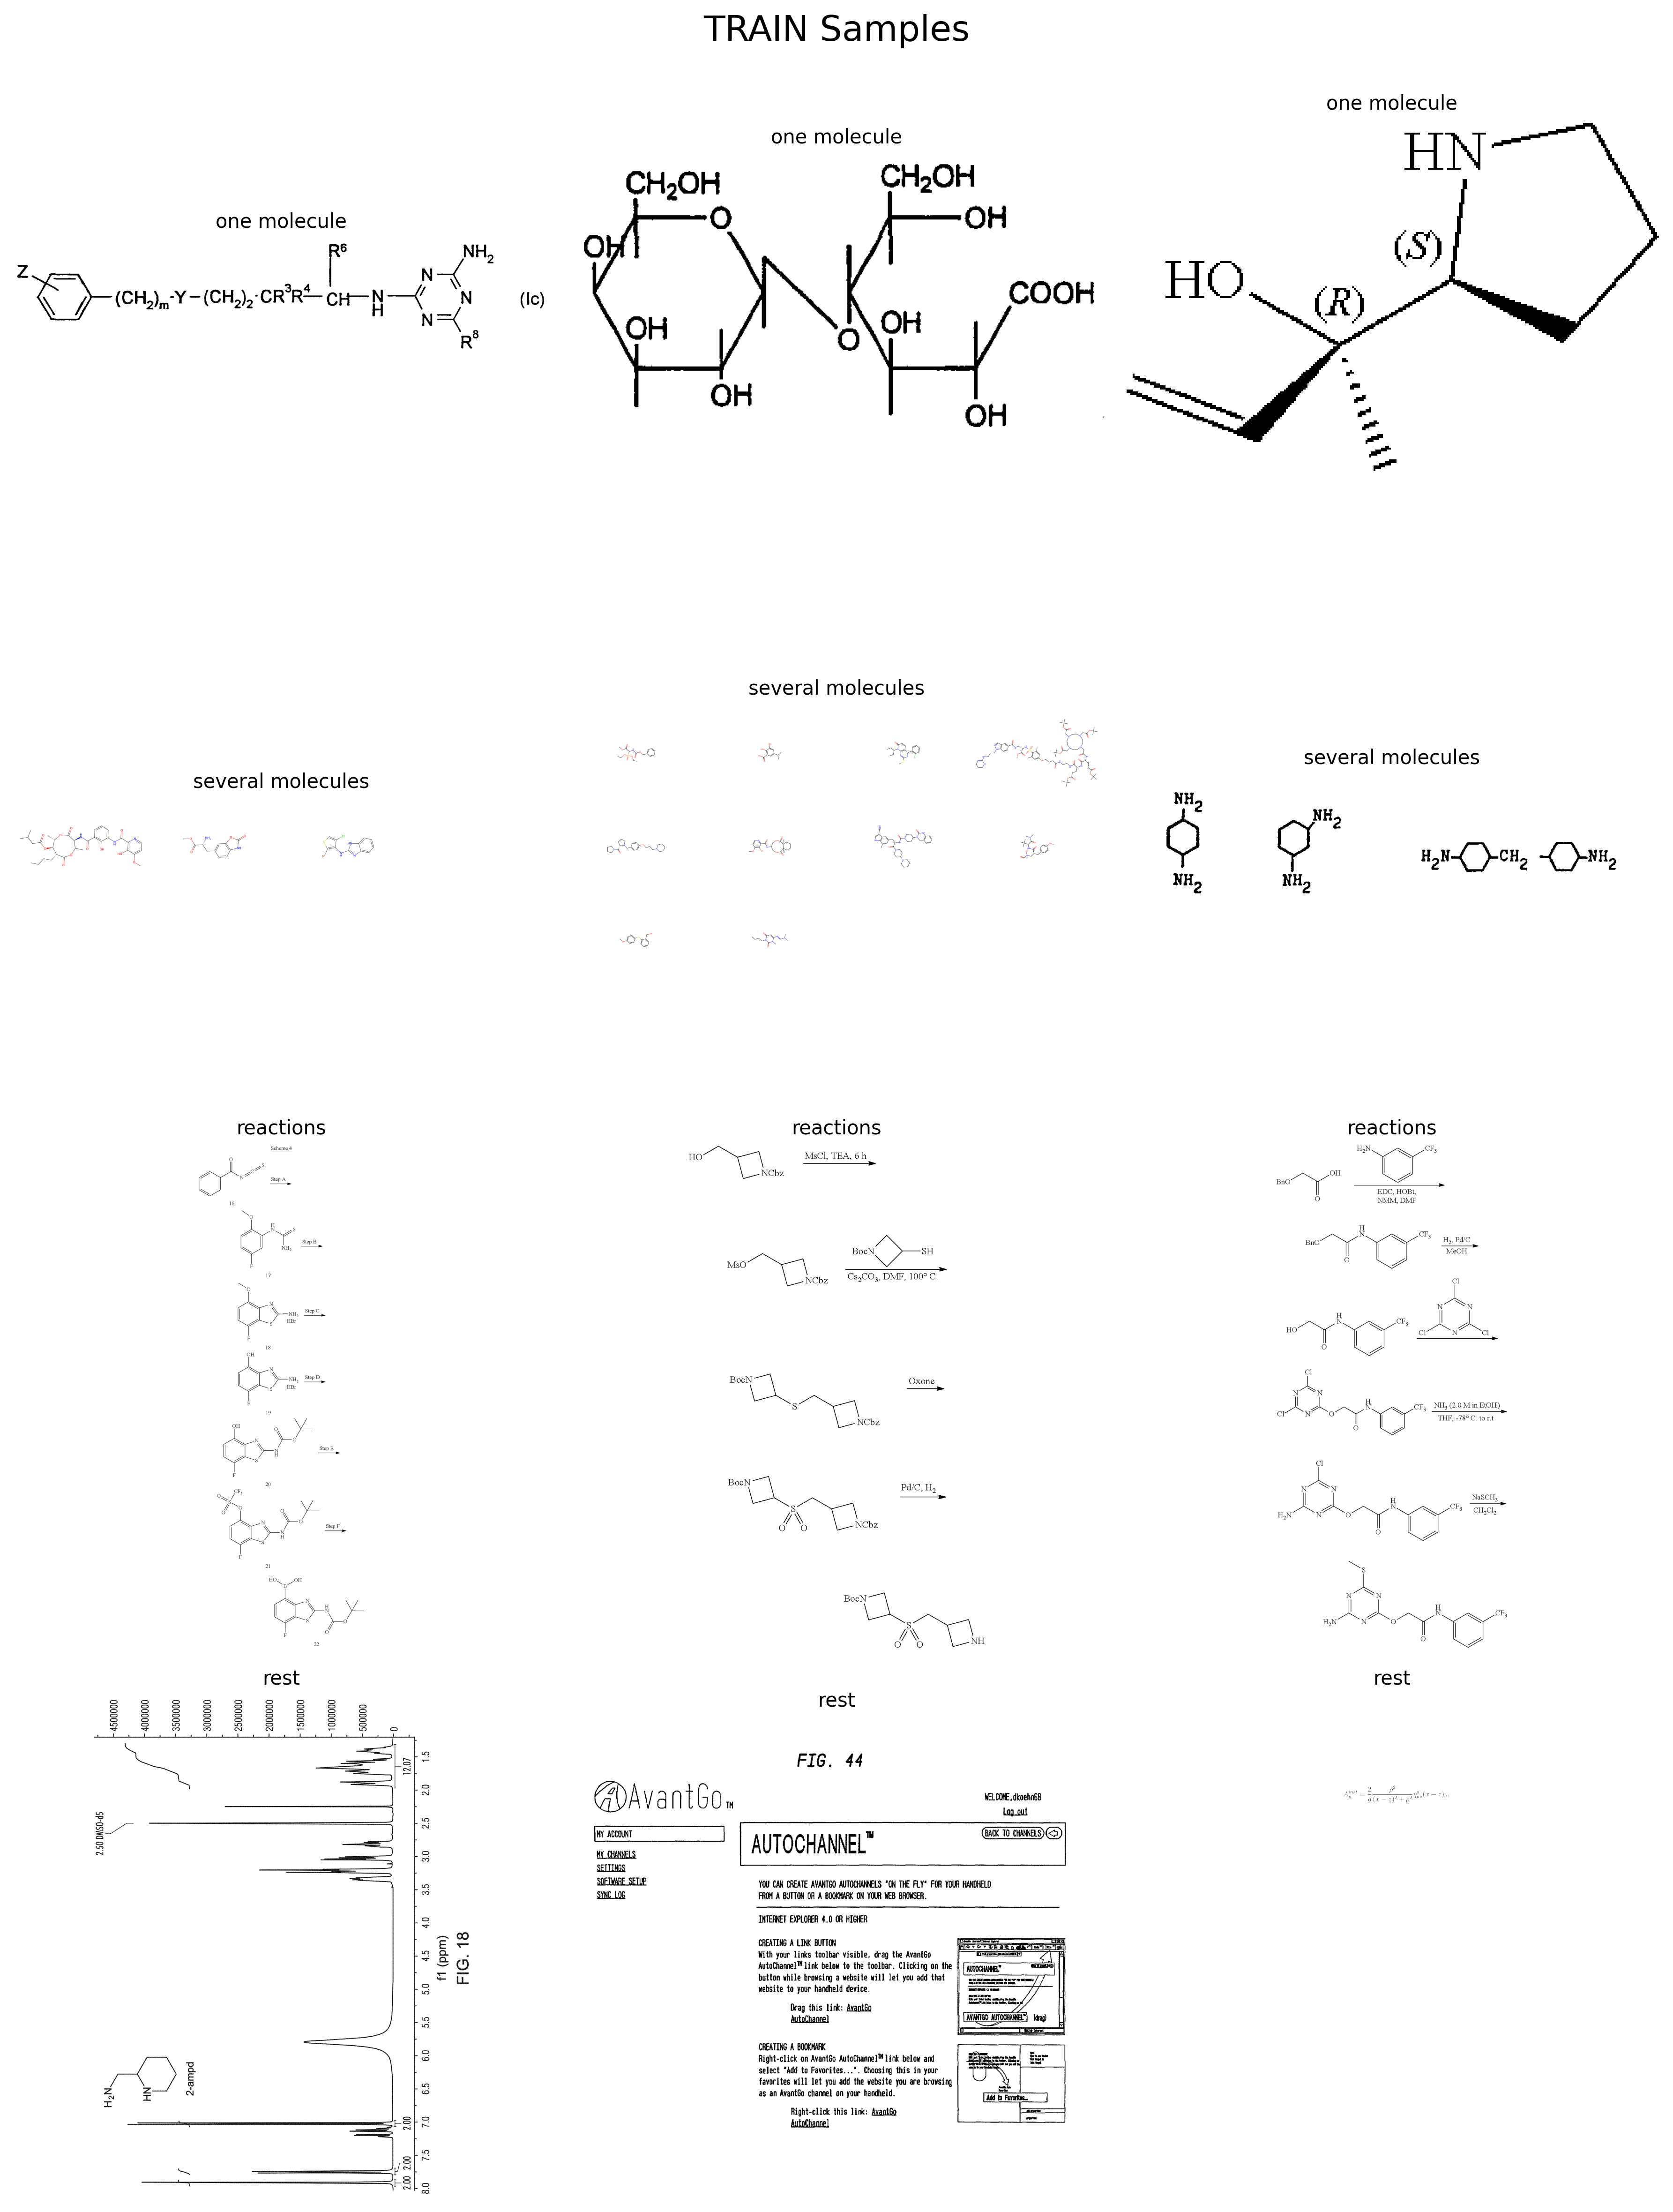
\includegraphics[width=0.72\textwidth]{chemical_classification_models/samples and distrubutation/raw dataset/train_samples.png}
  \caption*{\small\itshape\color{DarkGray}Sample images from the four chemical image classes}
\end{figure}

\vspace{0.6cm}

% Report info table
\renewcommand{\arraystretch}{1.4}
\begin{tabularx}{\textwidth}{>{\bfseries\color{NavyBlue}\sffamily}l X}
  \toprule
  Task       & Chemical Image Classification using Deep Learning \\
  Platform   & Google Colab (T4 GPU) + TensorFlow 2.20.0 \\
  Dataset    & Patent Chemical Images --- 4 Classes, 16,000 Images \\
  Models     & VGG16, DenseNet121, ResNet50V2, InceptionV3, MobileNetV2, \\
             & Xception, EfficientNetB4, ConvNeXtTiny, Custom CNN \\
  Submitted  & July 2026 \\
  \bottomrule
\end{tabularx}

\vfill
{\color{NavyBlue}\rule{\textwidth}{2.5pt}}
\end{titlepage}

% ==============================================================
%  TABLE OF CONTENTS
% ==============================================================
\newpage
\pagenumbering{roman}
\thispagestyle{plain}
{\sffamily\tableofcontents}
\newpage

% ==============================================================
%  ABSTRACT
% ==============================================================
\begin{tcolorbox}[
  enhanced,
  colback=NavyBlue!5!white,
  colframe=NavyBlue,
  title={\sffamily\bfseries Abstract},
  fonttitle=\large,
  arc=3pt, boxrule=1pt,
  left=12pt, right=12pt, top=8pt, bottom=8pt
]
This report presents a complete deep learning pipeline for classifying chemical images extracted from scientific publications and patent documents. The dataset contains \textbf{16,000 images} distributed equally across four classes: \textit{one\_molecule}, \textit{reactions}, \textit{rest}, and \textit{several\_molecules}. Eight state-of-the-art pre-trained convolutional neural networks were fine-tuned using transfer learning, alongside a custom CNN trained from scratch. All models were evaluated on a held-out test set of 1,600 images. \modelname{VGG16} achieved the highest performance with \textbf{91.06\% accuracy} and \textbf{AUC = 0.989}. Model interpretability was demonstrated using Grad-CAM heatmaps and LIME explanations.
\end{tcolorbox}
\vspace{1em}

\pagenumbering{arabic}

% ==============================================================
%  SECTION 1: INTRODUCTION
% ==============================================================
\section{Introduction \& Task Requirements}

This report documents a complete deep learning research pipeline for classifying chemical images extracted from scientific publications and patent documents. The dataset contains four distinct categories of chemical imagery, and the objective was to design, train, and rigorously evaluate multiple deep learning architectures --- both pre-trained transfer learning models and a custom-built CNN.

\subsection{Assigned and Performed Tasks}

\begin{itemize}[leftmargin=1.6em, itemsep=4pt]
  \item Show sample images from every class.
  \item Show class-wise image quantity across train/validation/test sets using a bar plot.
  \item Perform image preprocessing and data augmentation.
  \item Use pre-trained models: VGG16, DenseNet121, ResNet50V2, InceptionV3, MobileNetV2, Xception, EfficientNetB4, and ConvNeXtTiny --- with architectural modifications.
  \item Build and train a Custom CNN; ensemble models if required.
  \item Show model summaries.
  \item Plot accuracy and loss curves for training and validation sets.
  \item Compute Accuracy, Precision, Recall, F1-Score, Confusion Matrix, AUC, and ROC Curves.
  \item Generate Grad-CAM heatmaps to visualise model attention regions.
  \item Generate LIME explanations for model predictions.
\end{itemize}

% ==============================================================
%  SECTION 2: DATASET OVERVIEW
% ==============================================================
\section{Dataset Overview \& Directory Structure}

The dataset consists of chemical images sourced from patent documents and scientific journals. Images were standardised to PNG format before training. The dataset is split into three sets: Training, Validation, and Test --- with perfectly balanced class distribution across all splits.

\subsection{Class Descriptions}

\begin{table}[H]
\centering
\caption{Class Descriptions}
\label{tab:class_desc}
\begin{tabularx}{\textwidth}{>{\bfseries\color{NavyBlue}}l X}
  \toprule
  Class Name & Description \\
  \midrule
  one\_molecule      & Images containing a single molecular structure or compound diagram. \\
  reactions          & Images depicting chemical reactions with reagents, arrows, and products. \\
  rest               & Other chemical-related images not fitting the above categories. \\
  several\_molecules & Images containing multiple molecular structures arranged together. \\
  \bottomrule
\end{tabularx}
\end{table}

\subsection{Dataset Split Summary}

\begin{table}[H]
\centering
\caption{Dataset Split Summary}
\label{tab:dataset_split}
\rowcolors{2}{LightGray}{white}
\begin{tabular}{l c c c c c}
  \toprule
  \textbf{Split} & \textbf{one\_molecule} & \textbf{reactions} & \textbf{rest} & \textbf{several\_molecules} & \textbf{Total} \\
  \midrule
  Train           & 3,200 & 3,200 & 3,200 & 3,200 & 12,800 \\
  Validation      & 400   & 400   & 400   & 400   & 1,600  \\
  Test            & 400   & 400   & 400   & 400   & 1,600  \\
  \midrule
  \textbf{Grand Total} & \textbf{4,000} & \textbf{4,000} & \textbf{4,000} & \textbf{4,000} & \textbf{16,000} \\
  \bottomrule
\end{tabular}
\end{table}

\subsection{Directory Structure}

\begin{lstlisting}[language=sh, numbers=none, caption={Dataset Folder Hierarchy}]
dataset_png/
  |-- train/
  |     |-- one_molecule/      (3,200 images)
  |     |-- reactions/         (3,200 images)
  |     |-- rest/              (3,200 images)
  |     `-- several_molecules/ (3,200 images)
  |-- validation/
  |     `-- [400 images per class]
  `-- test/
        `-- [400 images per class]
\end{lstlisting}

% ==============================================================
%  SECTION 3: SAMPLE IMAGES
% ==============================================================
\section{Sample Images from Every Class}

Random sample images were displayed from each of the four classes across all three dataset splits. A grid of 4 samples per class was generated for each split using \code{matplotlib}.

\begin{lstlisting}[language=Python, caption={Sample Image Grid Generation}]
SAMPLES_PER_CLASS = 4
fig, axes = plt.subplots(NUM_CLASSES, SAMPLES_PER_CLASS, figsize=(16, 16))
fig.suptitle('Training Set Samples', fontsize=22, fontweight='bold')
for row, cls in enumerate(CLASSES):
    cls_dir = os.path.join(TRAIN_DIR, cls)
    imgs    = get_images(cls_dir)
    chosen  = random.sample(imgs, min(SAMPLES_PER_CLASS, len(imgs)))
    for col, path in enumerate(chosen):
        ax.imshow(load_image_rgb(path))
plt.tight_layout()
plt.savefig('train_samples.png', dpi=150)
\end{lstlisting}

\subsection{Raw Training Set Samples}

\begin{figure}[H]
  \centering
  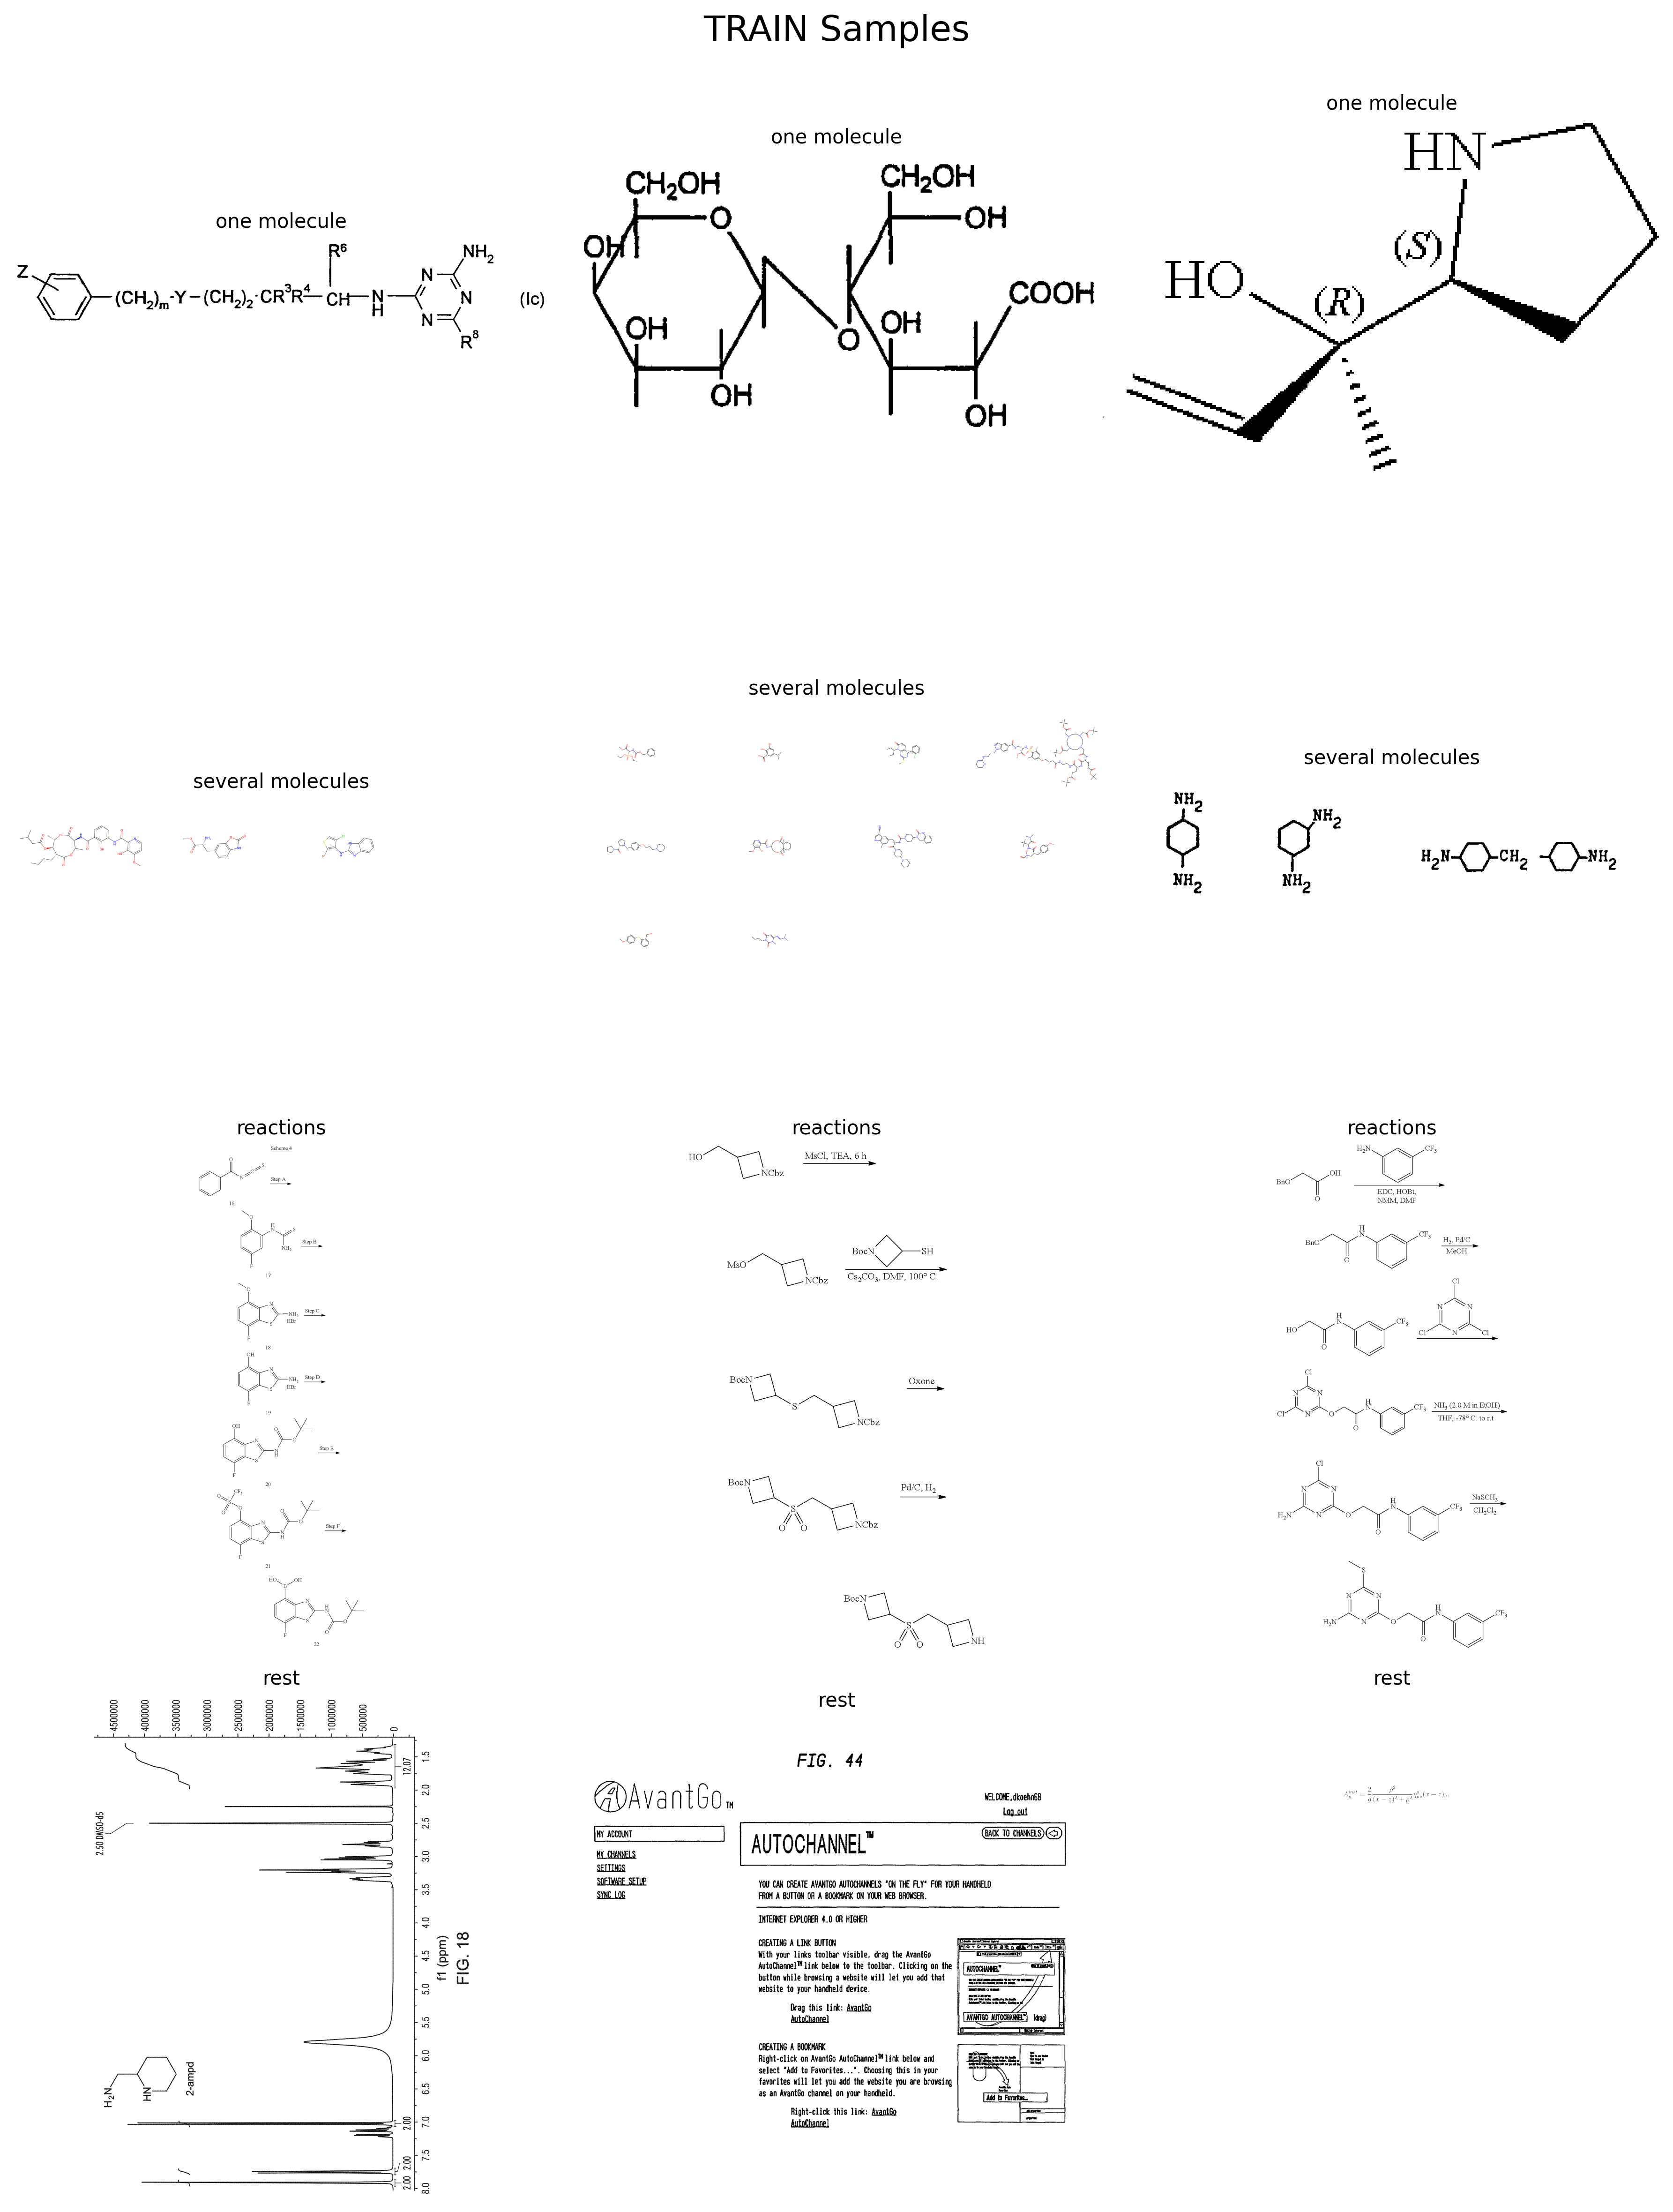
\includegraphics[width=0.88\textwidth]{chemical_classification_models/samples and distrubutation/raw dataset/train_samples.png}
  \caption{Raw Training Set --- 4 samples $\times$ 4 classes}
  \label{fig:train_samples_raw}
\end{figure}

\subsection{Raw Validation Set Samples}

\begin{figure}[H]
  \centering
  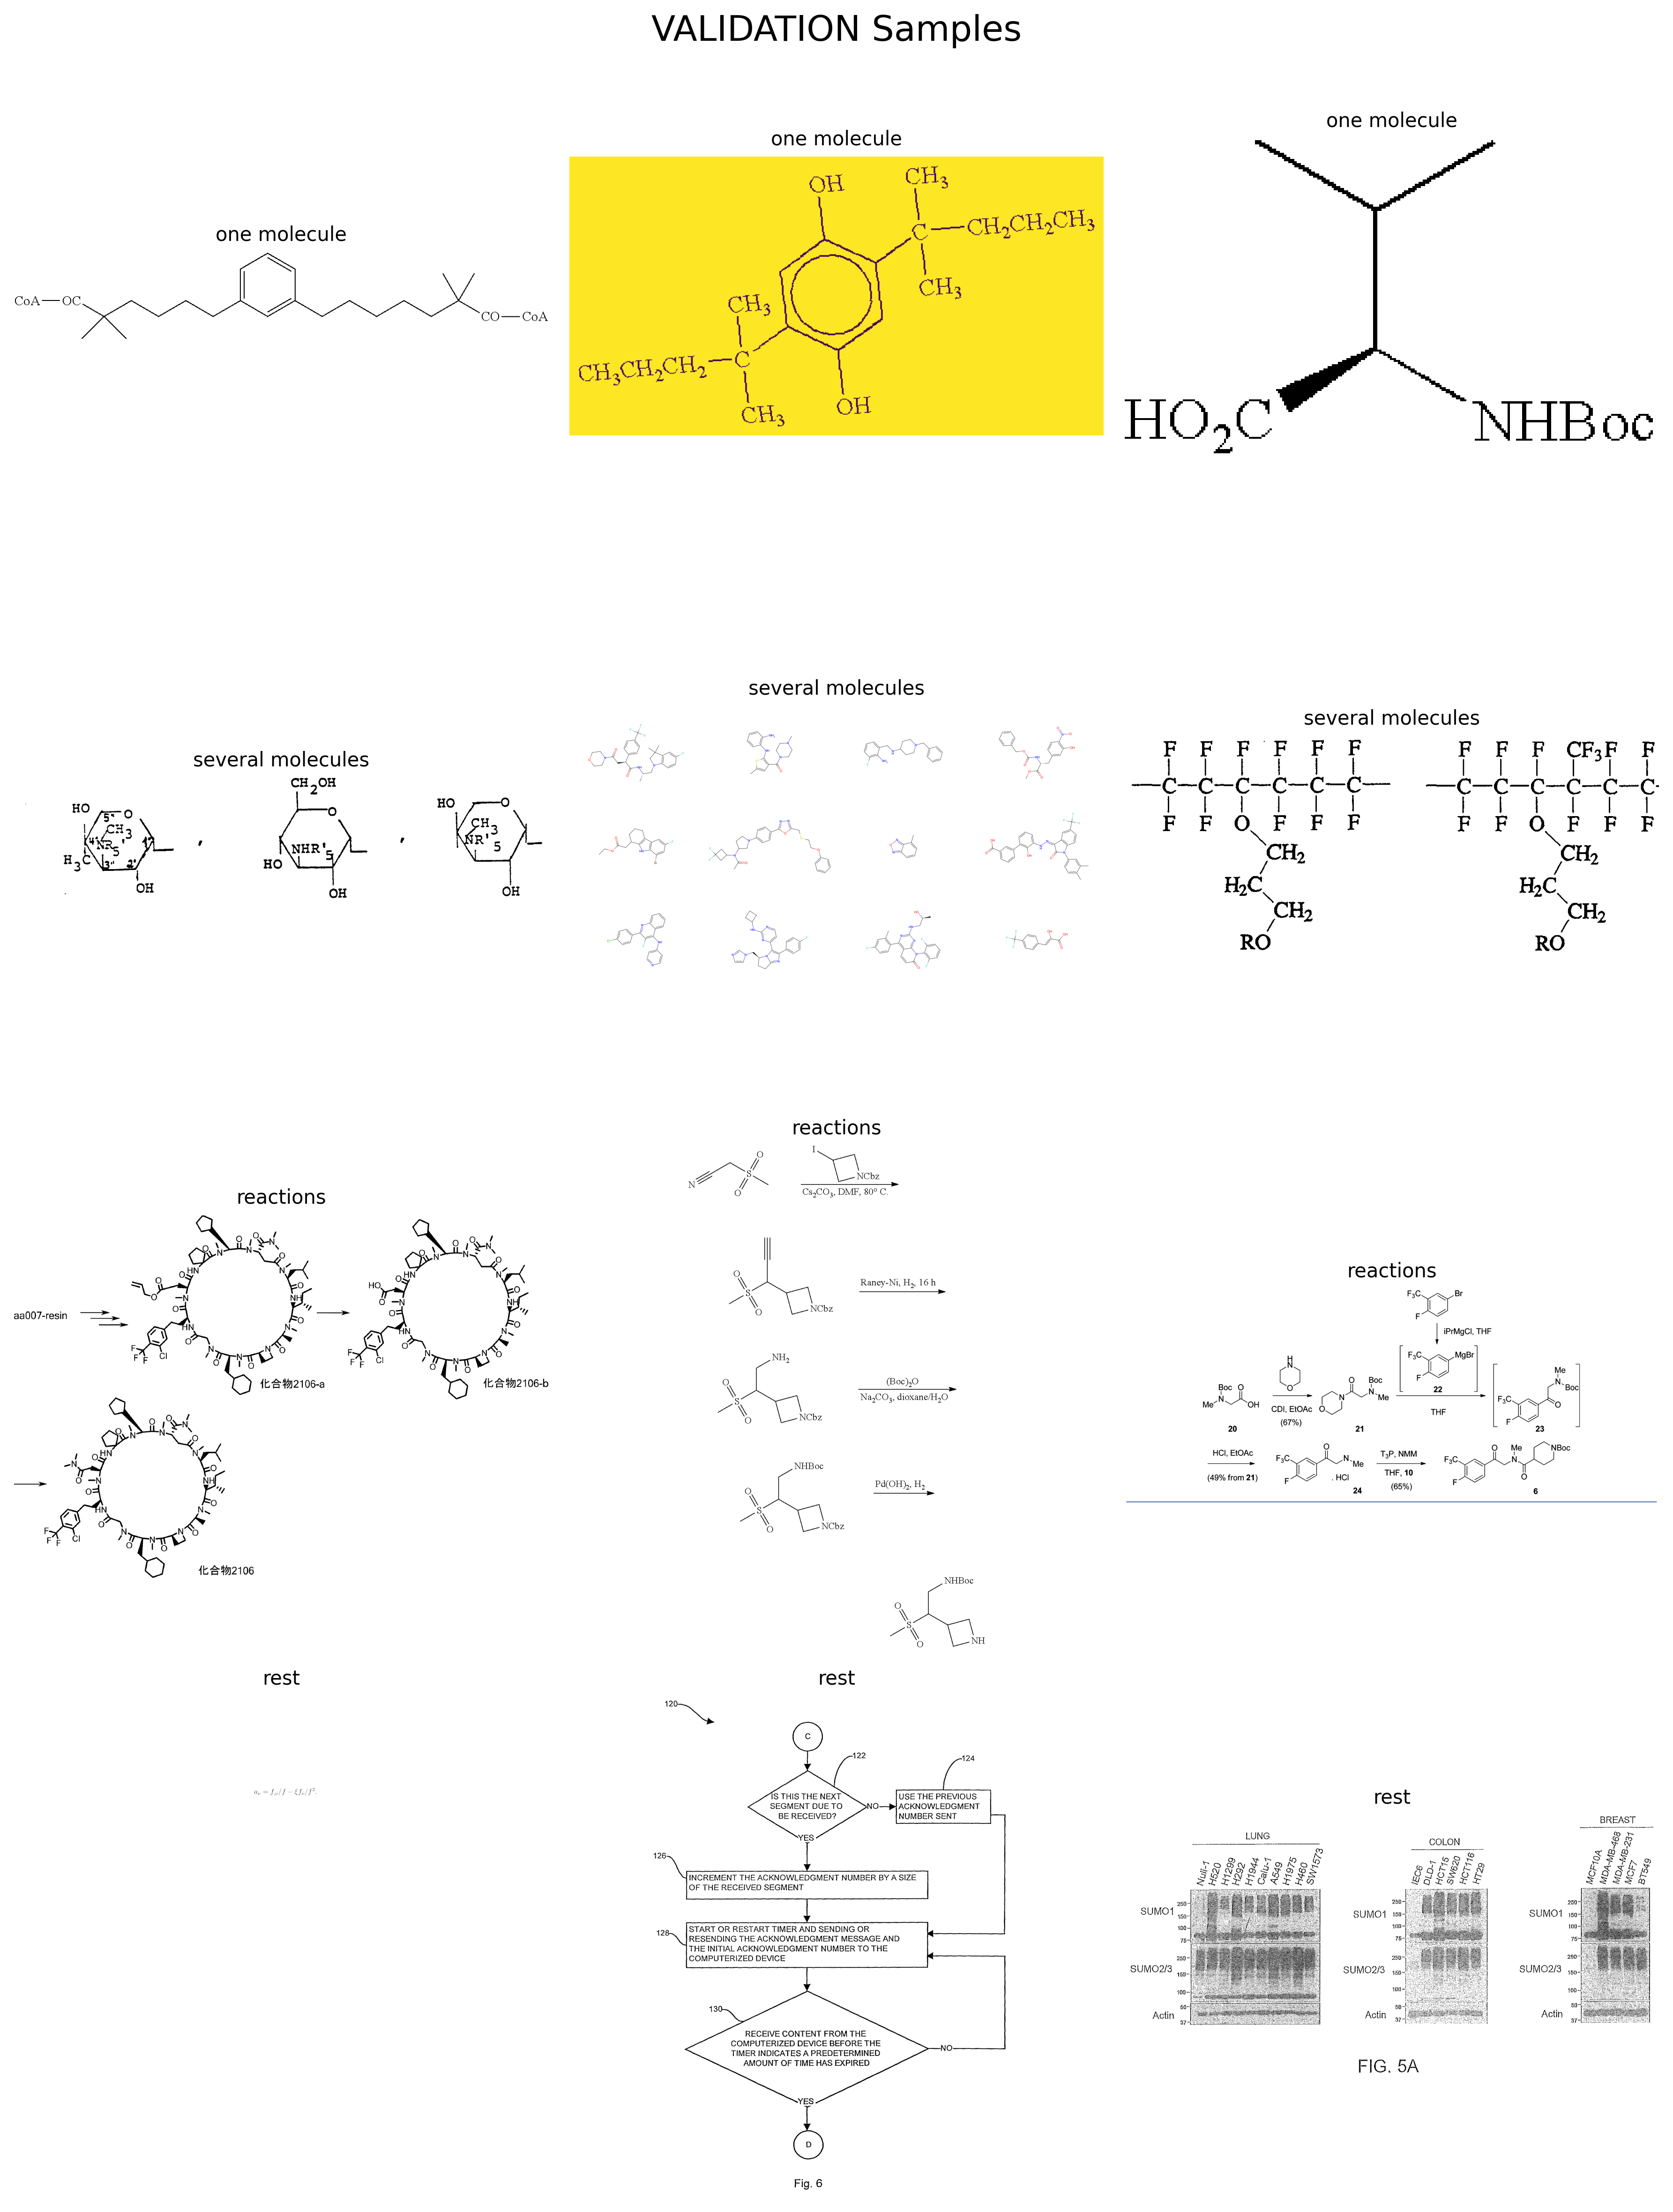
\includegraphics[width=0.88\textwidth]{chemical_classification_models/samples and distrubutation/raw dataset/validation_samples.png}
  \caption{Raw Validation Set --- 4 samples $\times$ 4 classes}
  \label{fig:val_samples_raw}
\end{figure}

\subsection{Raw Test Set Samples}

\begin{figure}[H]
  \centering
  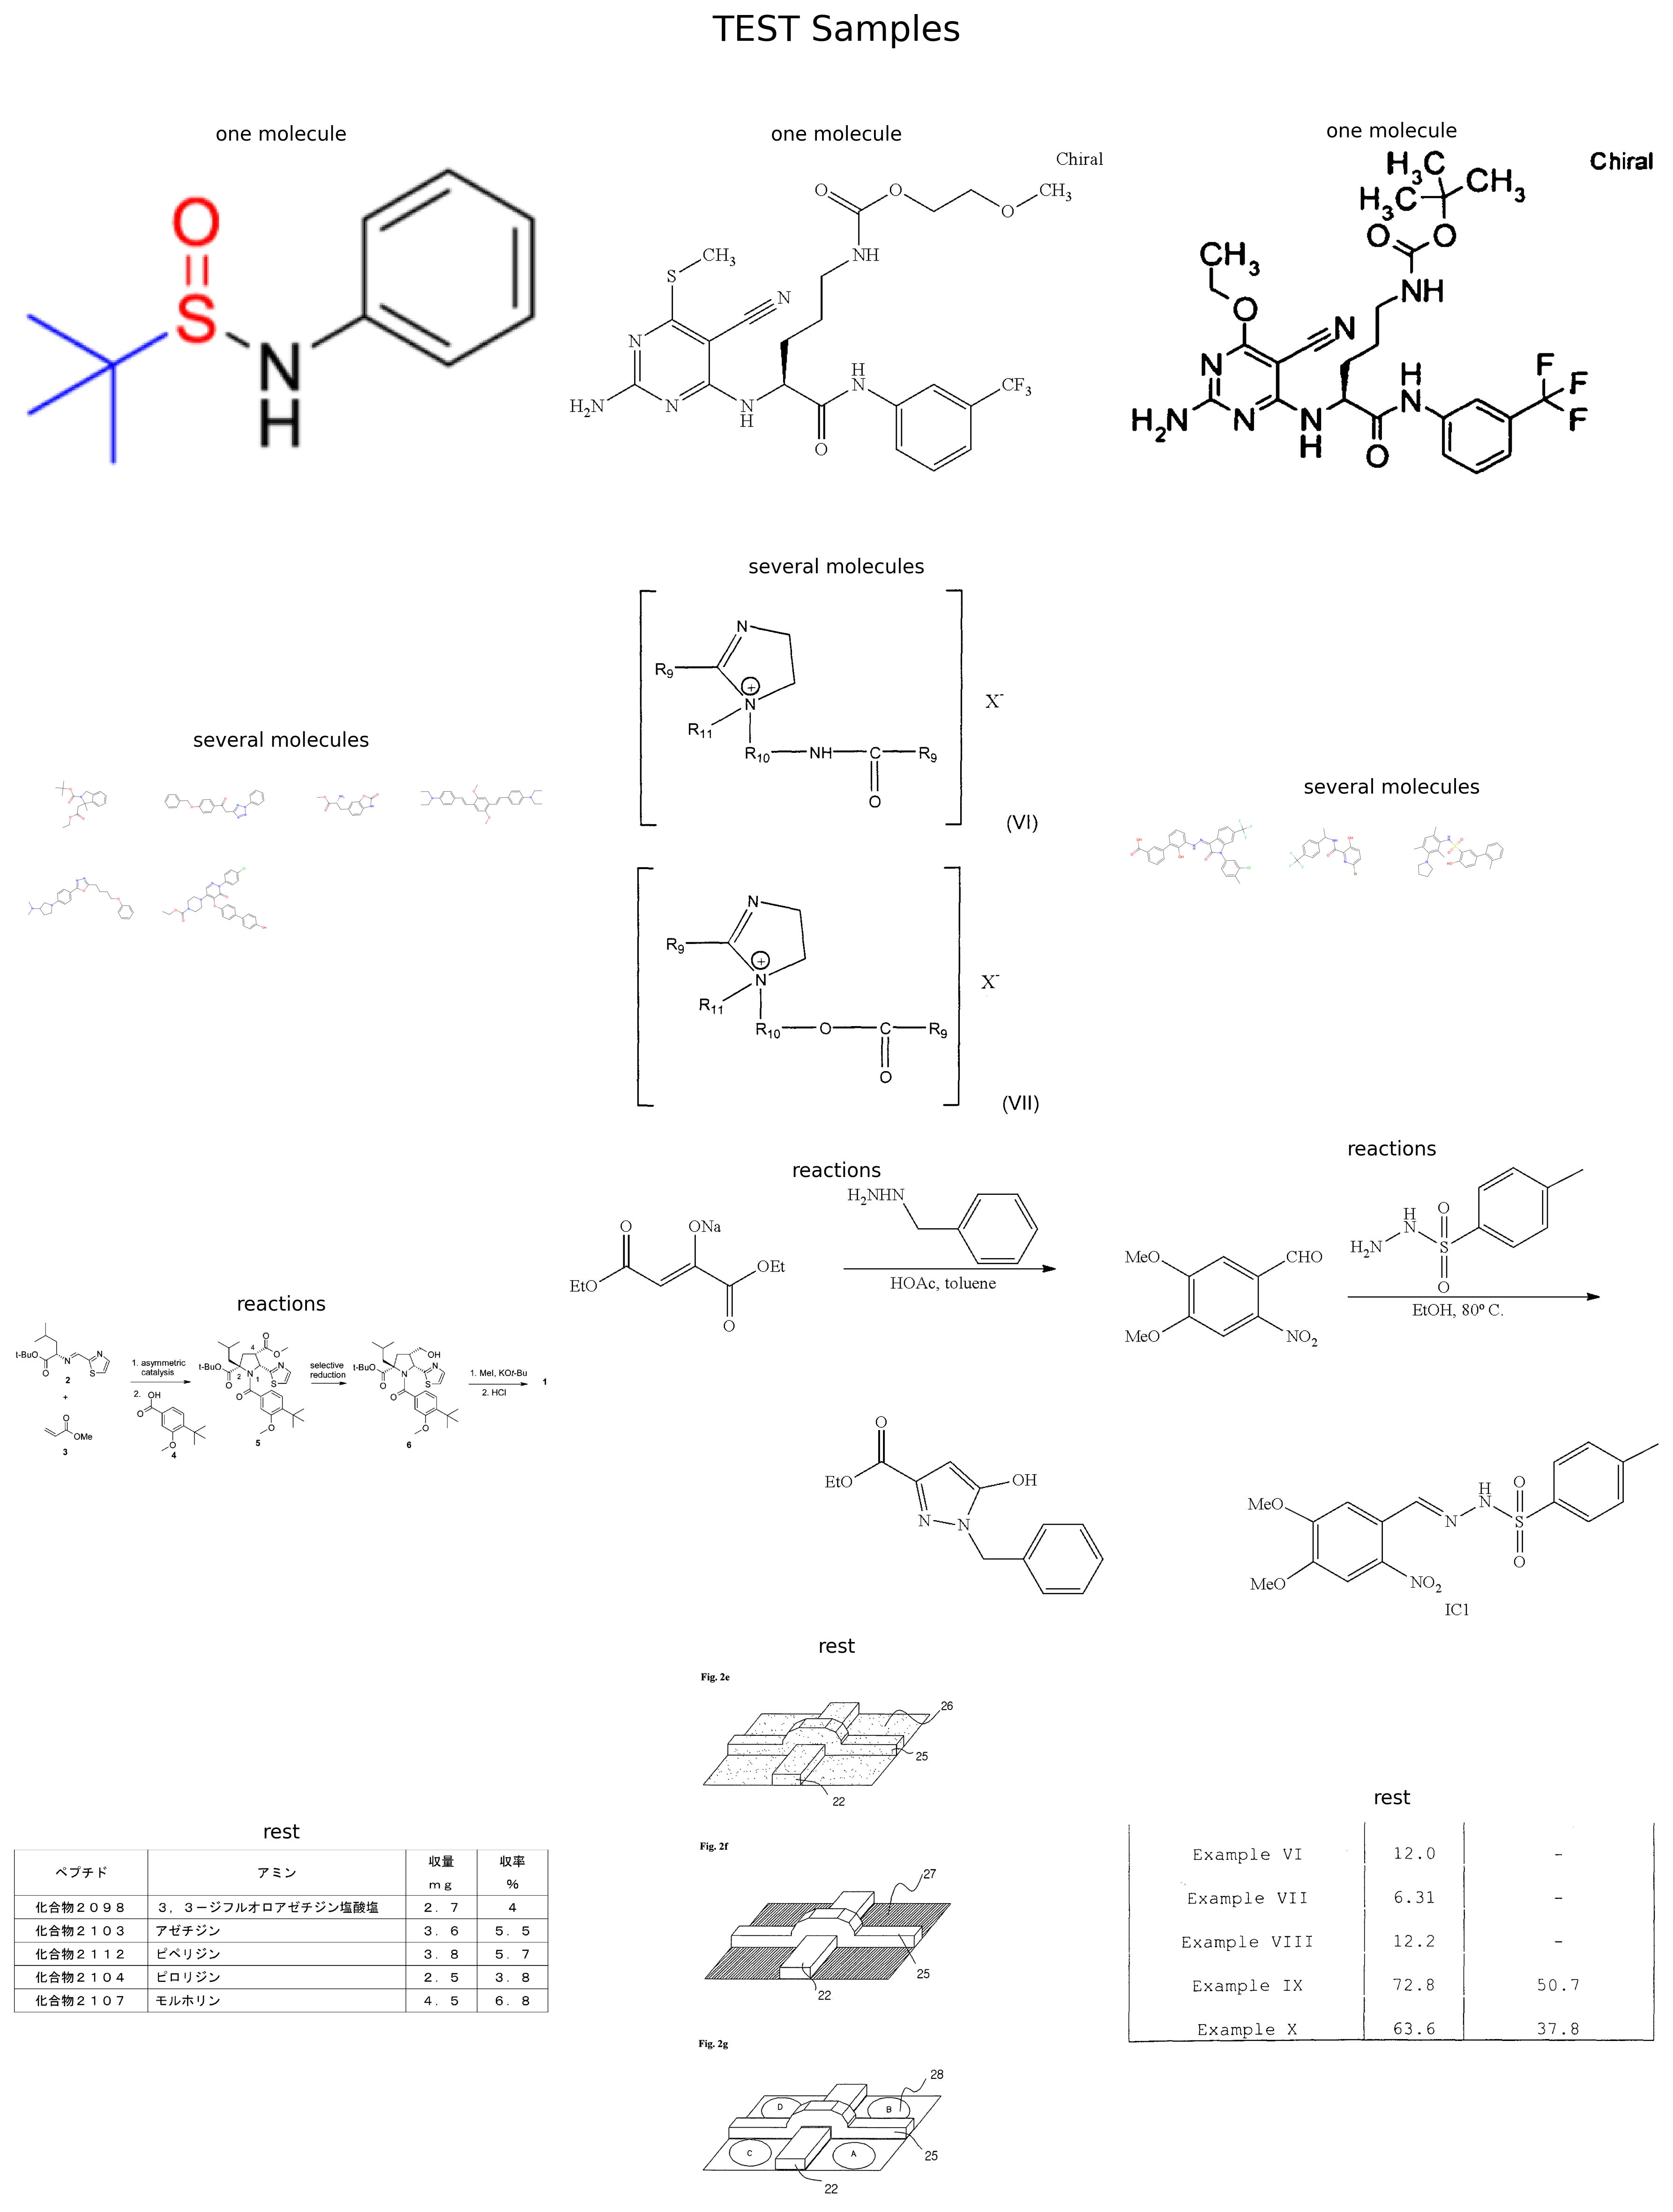
\includegraphics[width=0.88\textwidth]{chemical_classification_models/samples and distrubutation/raw dataset/test_samples.png}
  \caption{Raw Test Set --- 4 samples $\times$ 4 classes}
  \label{fig:test_samples_raw}
\end{figure}

% ==============================================================
%  SECTION 4: BAR PLOT
% ==============================================================
\section{Class-wise Image Distribution (Bar Plot)}

A grouped bar chart was produced showing the number of images per class across all three splits. The dataset is \textbf{perfectly balanced} --- every class has equal image counts in each split, ensuring unbiased model training and fair evaluation.

\begin{lstlisting}[language=Python, caption={Class Distribution Bar Plot}]
x = np.arange(len(CLASSES))  ;  width = 0.25
splits = ['train', 'validation', 'test']
colors = ['#2196F3', '#4CAF50', '#FF9800']
for idx, (split, color) in enumerate(zip(splits, colors)):
    values = [counts[split][cls] for cls in CLASSES]
    ax.bar(x + idx*width, values, width, label=split.capitalize(), color=color)
ax.set_title('Class-wise Image Distribution Across Splits')
plt.savefig('class_distribution.png', dpi=150)
\end{lstlisting}

\begin{figure}[H]
  \centering
  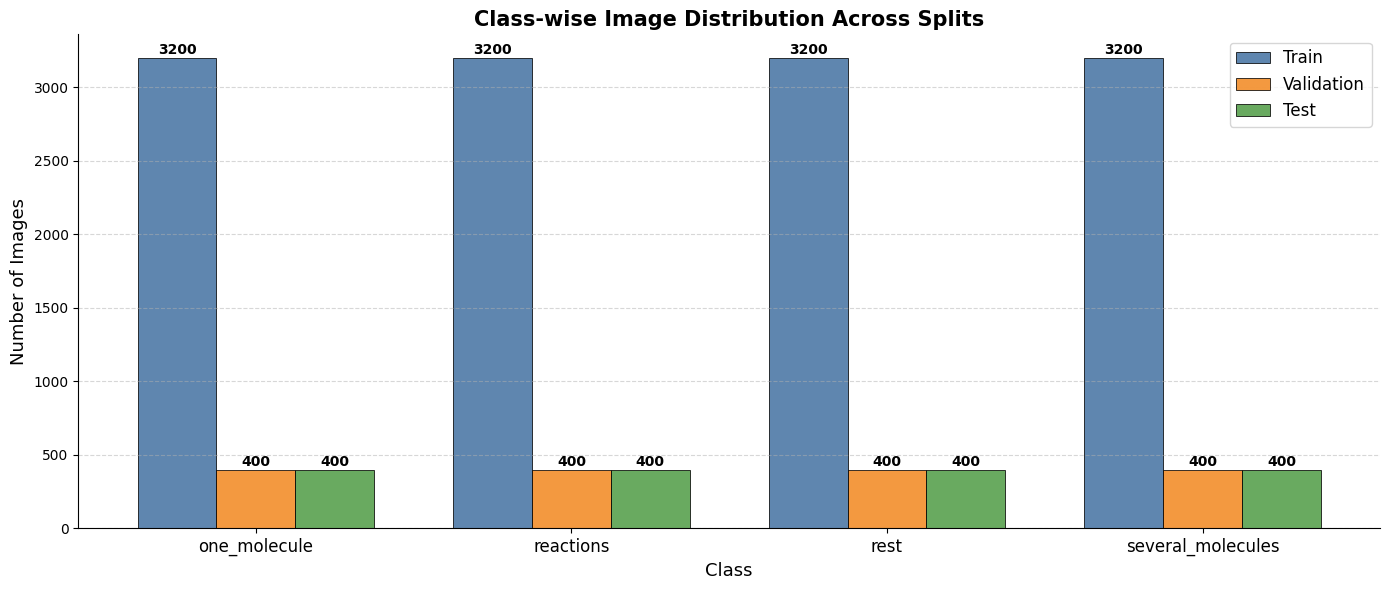
\includegraphics[width=0.82\textwidth]{chemical_classification_models/samples and distrubutation/raw dataset/class_distribution.png}
  \caption{Class-wise Image Distribution Across Train / Validation / Test Splits}
  \label{fig:class_dist}
\end{figure}

% ==============================================================
%  SECTION 5: PREPROCESSING & DATA AUGMENTATION
% ==============================================================
\section{Image Preprocessing \& Augmentation}

All images were standardised and augmented using the Keras \code{ImageDataGenerator} API. The following pipeline was applied exclusively to the training set to improve model generalisation and prevent overfitting:

\begin{table}[H]
\centering
\caption{Image Augmentation Parameters}
\label{tab:augmentation}
\rowcolors{2}{LightGray}{white}
\begin{tabularx}{\textwidth}{>{\bfseries\color{NavyBlue}}l X}
  \toprule
  Augmentation Parameter & Value / Setting \\
  \midrule
  Rescaling          & $1/255$ --- normalise pixel values to $[0,\,1]$ \\
  Rotation Range     & $\pm 20^{\circ}$ \\
  Width Shift Range  & 15\% of image width \\
  Height Shift Range & 15\% of image height \\
  Shear Range        & 10\% \\
  Zoom Range         & 20\% \\
  Horizontal Flip    & Enabled \\
  Vertical Flip      & Enabled \\
  Fill Mode          & Nearest \\
  Validation Split   & 20\% of training images \\
  \bottomrule
\end{tabularx}
\end{table}

\begin{lstlisting}[language=Python, caption={ImageDataGenerator Setup}]
train_datagen = ImageDataGenerator(
    rescale=1./255, rotation_range=20,
    width_shift_range=0.15, height_shift_range=0.15,
    shear_range=0.1, zoom_range=0.2,
    horizontal_flip=True, vertical_flip=True,
    validation_split=0.2, fill_mode='nearest'
)
# Generator streams
train_gen = ...flow_from_directory(..., subset='training')    # 10,240 images
val_gen   = ...flow_from_directory(..., subset='validation')  #  2,560 images
test_gen  = val_test_datagen.flow_from_directory(...)         #  1,600 images
\end{lstlisting}

\subsection{Preprocessed Class Distribution}

\begin{figure}[H]
  \centering
  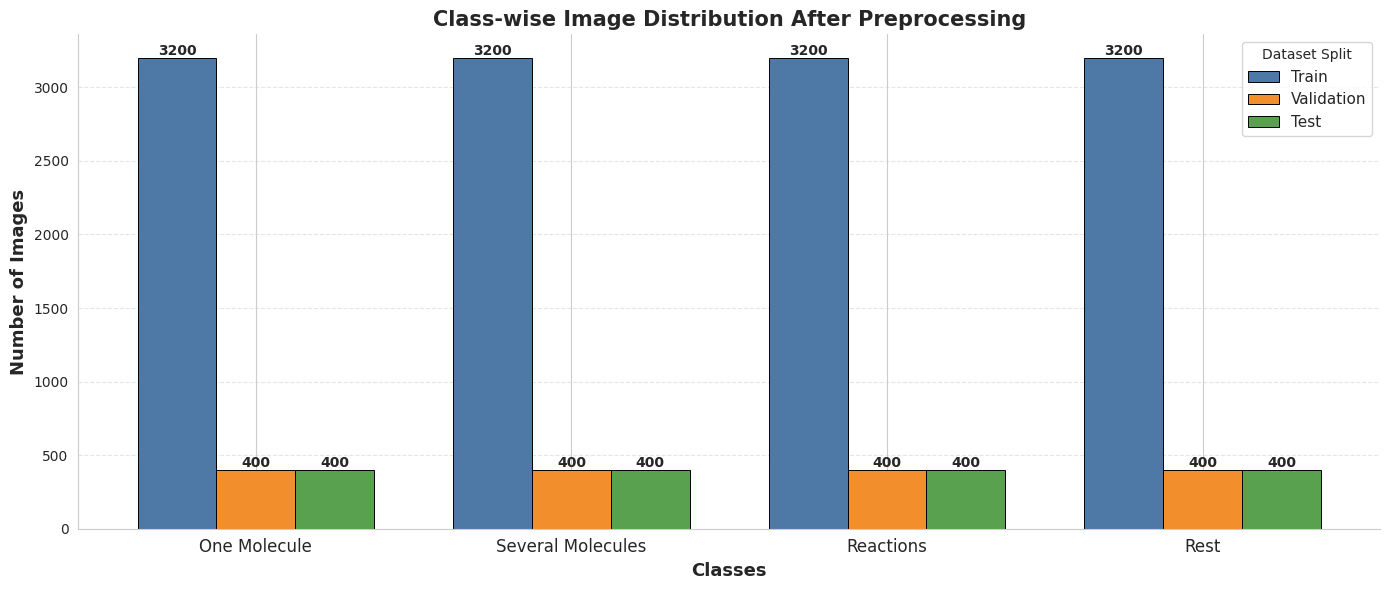
\includegraphics[width=0.82\textwidth]{chemical_classification_models/samples and distrubutation/preprocess dataset/Figure_Preprocessed_Class_Distribution.png}
  \caption{Preprocessed Dataset --- Class Distribution (Train / Validation / Test)}
  \label{fig:class_dist_prep}
\end{figure}

\subsection{Preprocessed Training Set Samples}

\begin{figure}[H]
  \centering
  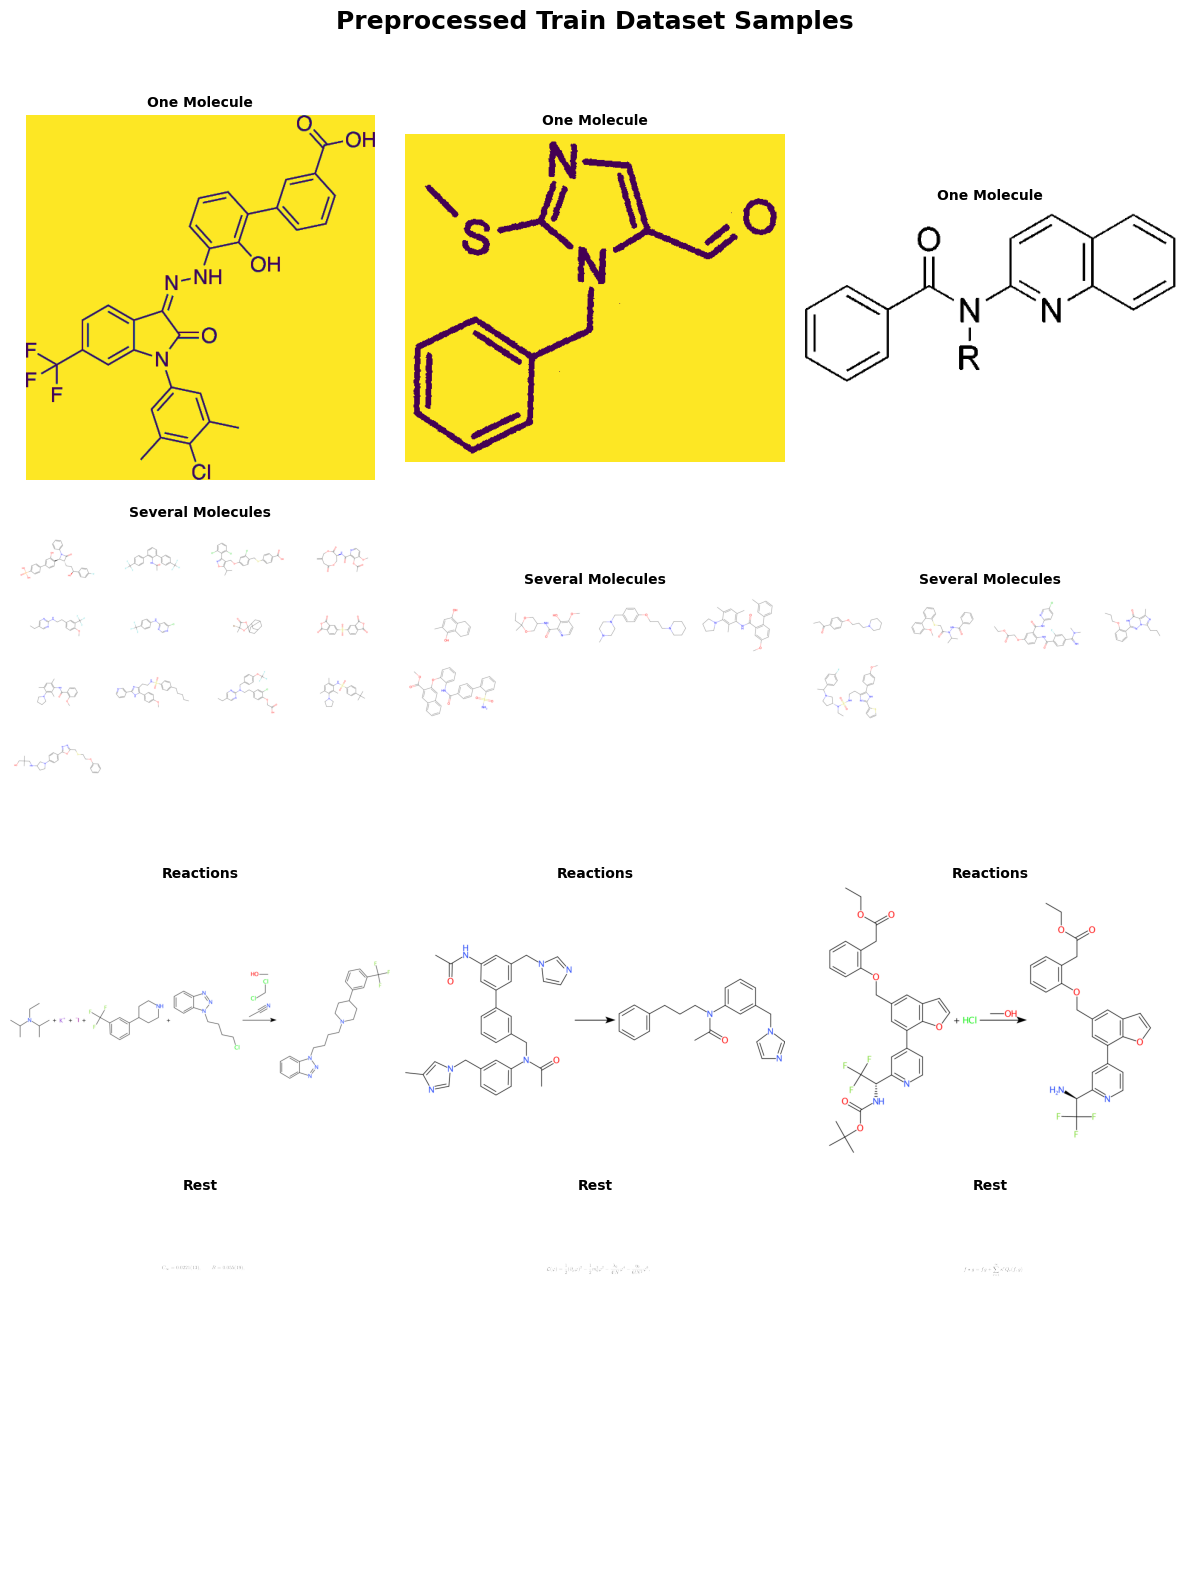
\includegraphics[width=0.88\textwidth]{chemical_classification_models/samples and distrubutation/preprocess dataset/train_preprocessed_samples.png}
  \caption{Preprocessed Training Set Samples --- 4 samples $\times$ 4 classes}
  \label{fig:train_samples_prep}
\end{figure}

\subsection{Preprocessed Validation Set Samples}

\begin{figure}[H]
  \centering
  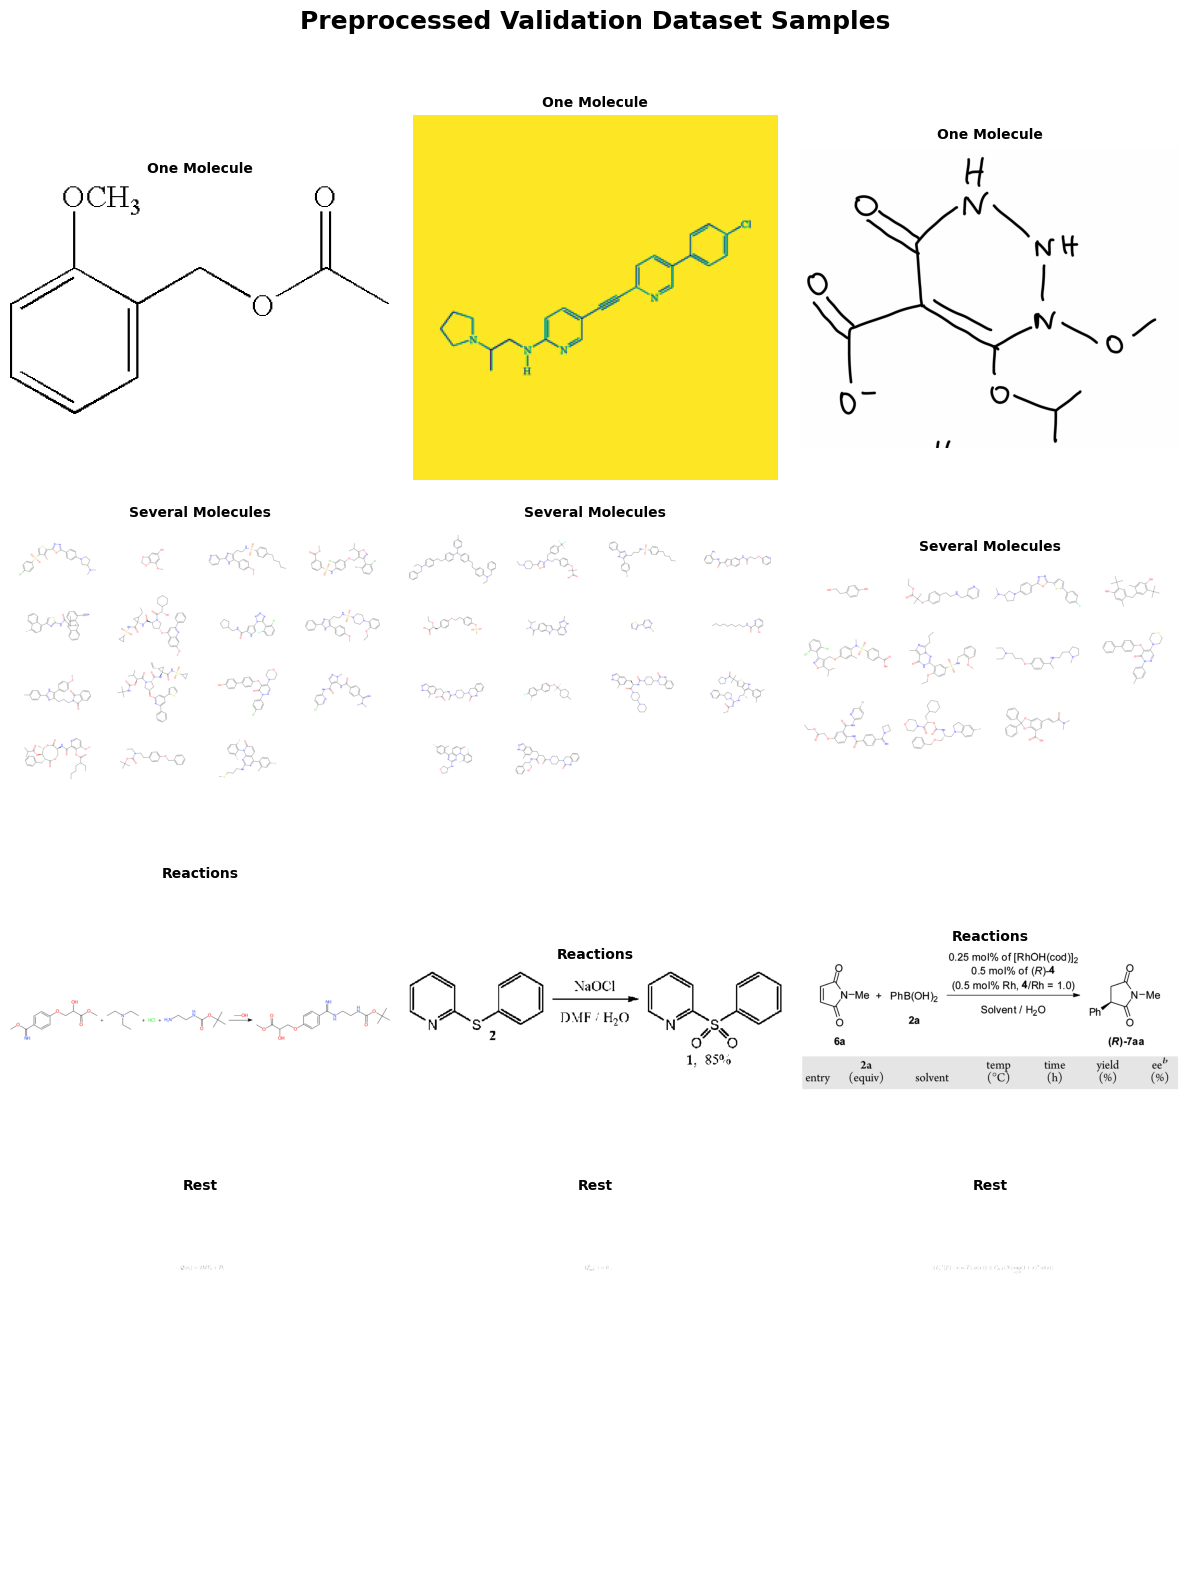
\includegraphics[width=0.88\textwidth]{chemical_classification_models/samples and distrubutation/preprocess dataset/validation_preprocessed_samples.png}
  \caption{Preprocessed Validation Set Samples --- 4 samples $\times$ 4 classes}
  \label{fig:val_samples_prep}
\end{figure}

\subsection{Preprocessed Test Set Samples}

\begin{figure}[H]
  \centering
  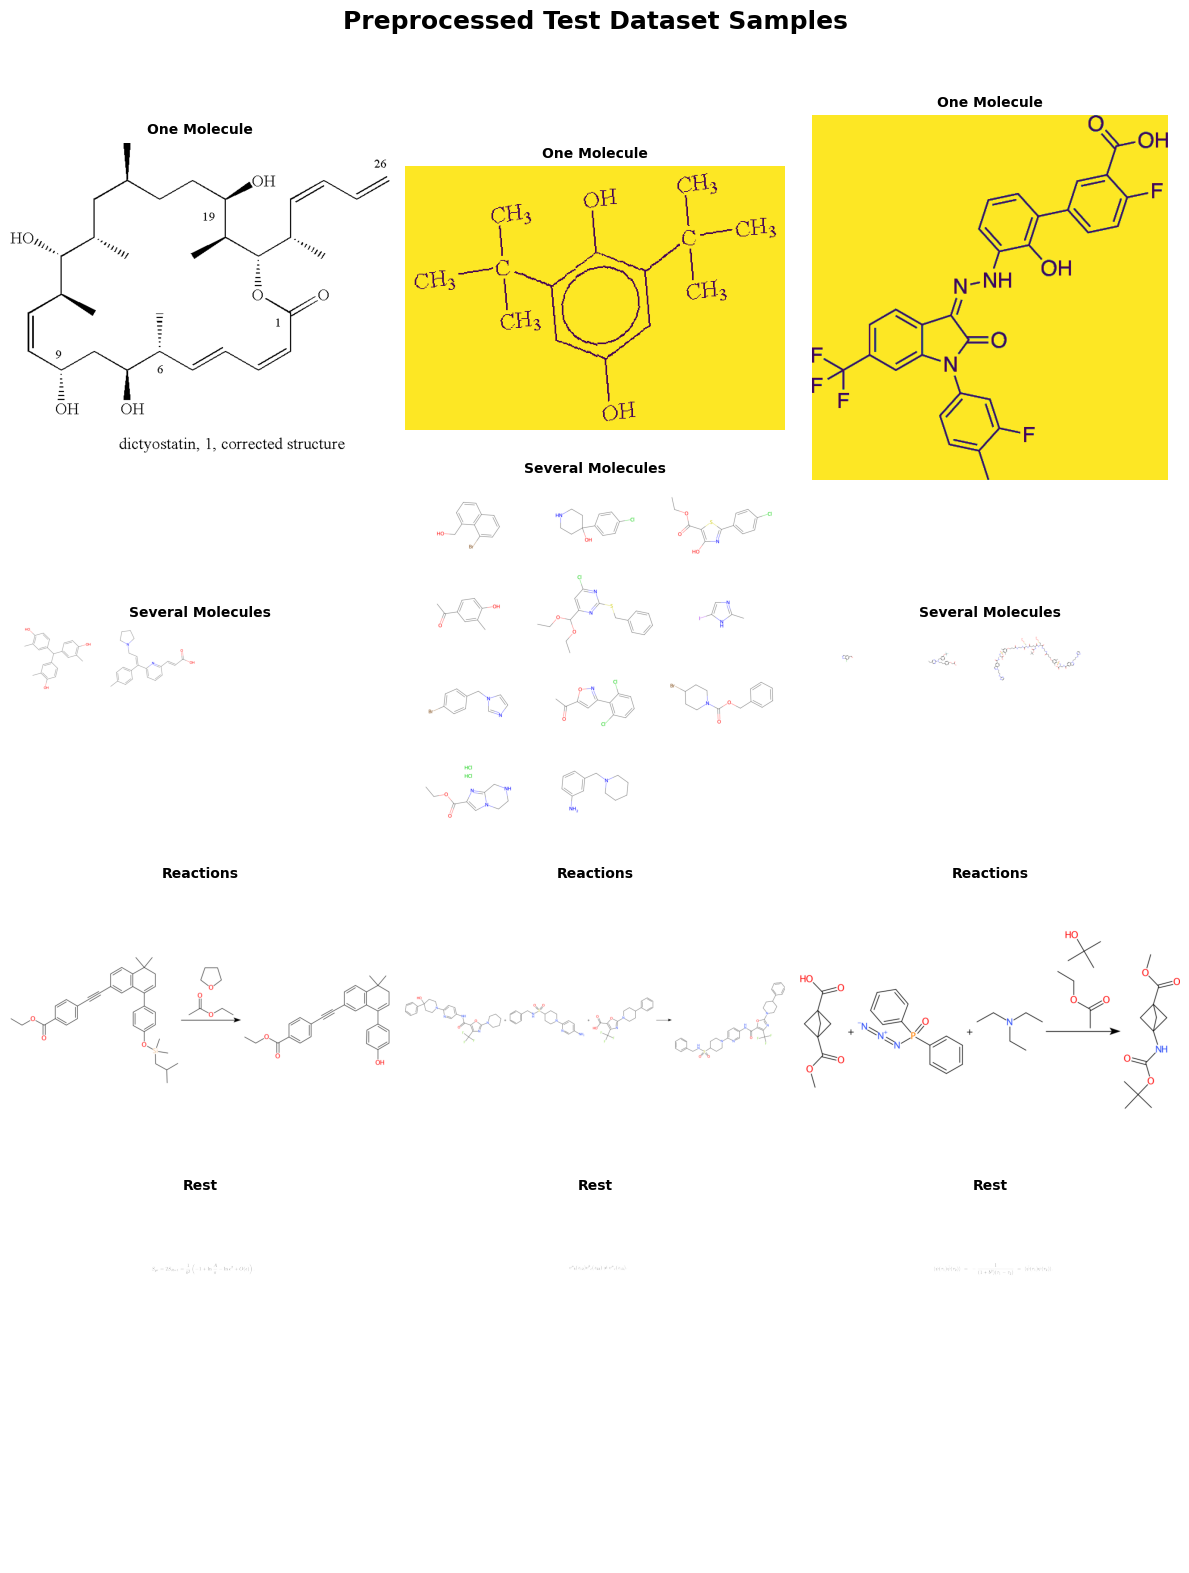
\includegraphics[width=0.88\textwidth]{chemical_classification_models/samples and distrubutation/preprocess dataset/test_preprocessed_samples.png}
  \caption{Preprocessed Test Set Samples --- 4 samples $\times$ 4 classes}
  \label{fig:test_samples_prep}
\end{figure}

% ==============================================================
%  SECTION 6: MODEL ARCHITECTURE
% ==============================================================
\section{Model Architecture \& Design}

\subsection{Transfer Learning Framework}

A unified function \code{build\_transfer\_model()} applies an identical classification head to every pre-trained backbone, ensuring a fair comparison across architectures. The classification head consists of:

\begin{itemize}[leftmargin=1.6em, itemsep=4pt]
  \item Pre-trained base (ImageNet weights, \code{include\_top=False})
  \item Global Average Pooling 2D
  \item Batch Normalization
  \item Dense(512, ReLU) + Dropout(0.5)
  \item Dense(256, ReLU) + Dropout(0.25)
  \item Dense(4, Softmax) --- output layer
\end{itemize}

\begin{lstlisting}[language=Python, caption={Unified Transfer Learning Builder Function}]
def build_transfer_model(base_model_fn, input_shape=(224,224,3),
                         num_classes=4, dropout=0.5, fine_tune_from=None):
    base = base_model_fn(weights='imagenet', include_top=False,
                         input_shape=input_shape)
    base.trainable = False
    inputs  = Input(shape=input_shape)
    x       = base(inputs, training=False)
    x       = GlobalAveragePooling2D()(x)
    x       = BatchNormalization()(x)
    x       = Dense(512, activation='relu')(x)
    x       = Dropout(0.5)(x)
    x       = Dense(256, activation='relu')(x)
    x       = Dropout(0.25)(x)
    outputs = Dense(num_classes, activation='softmax')(x)
    model   = Model(inputs, outputs)
    # Selective fine-tuning of last N layers
    model.compile(optimizer=Adam(1e-4),
                  loss='categorical_crossentropy', metrics=['accuracy'])
    return model
\end{lstlisting}

\subsection{Pre-trained Models Used}

\begin{table}[H]
\centering
\caption{Pre-trained Models Configuration}
\label{tab:pretrained_models_desc}
\rowcolors{2}{LightGray}{white}
\begin{tabularx}{\textwidth}{>{\bfseries}l l l X}
  \toprule
  Model          & Input Size         & Epochs / Fine-tune      & Key Characteristic \\
  \midrule
  VGG16          & 224$\times$224     & 5 / fine\_tune\_from=8  & Oxford VGG 16-layer deep CNN \\
  DenseNet121    & 224$\times$224     & 5 / fine\_tune\_from=20 & Dense skip connections between all layers \\
  ResNet50V2     & 224$\times$224     & 5 / fine\_tune\_from=20 & Improved residual learning (V2) \\
  InceptionV3    & 299$\times$299     & 3 / fine\_tune\_from=20 & Multi-scale inception modules \\
  MobileNetV2    & 224$\times$224     & 3 / fine\_tune\_from=30 & Lightweight depthwise separable convolutions \\
  Xception       & 299$\times$299     & 5 / fine\_tune\_from=20 & Extreme inception --- full depthwise convolutions \\
  EfficientNetB4 & 224$\times$224     & 5 / fine\_tune\_from=30 & Compound width/depth/resolution scaling \\
  ConvNeXtTiny   & 224$\times$224     & 5 / fine\_tune\_from=20 & Modern pure ConvNet, ViT-inspired design \\
  \bottomrule
\end{tabularx}
\end{table}

\subsection{Custom CNN Architecture}

A deep custom CNN was built from scratch with 4 convolutional blocks followed by a classification head:

\begin{lstlisting}[language=Python, caption={Custom CNN Architecture}]
def build_custom_cnn(input_shape=(224,224,3), num_classes=4):
    # Block 1:  Conv2D(64)  x2 + BN + MaxPool + Dropout(0.20)
    # Block 2:  Conv2D(128) x2 + BN + MaxPool + Dropout(0.25)
    # Block 3:  Conv2D(256) x2 + BN + MaxPool + Dropout(0.30)
    # Block 4:  Conv2D(512) x2 + BN + MaxPool + Dropout(0.35)
    # Head:     GlobalAvgPool -> Dense(512)+BN+Drop(0.5)
    #           -> Dense(256)+Drop(0.3) -> Dense(4, softmax)
    model.compile(optimizer=Adam(1e-3), loss='categorical_crossentropy')
\end{lstlisting}

% ==============================================================
%  SECTION 7: TRAINING CONFIGURATION
% ==============================================================
\section{Training Configuration \& Callbacks}

\begin{table}[H]
\centering
\caption{Training Parameters}
\label{tab:training_params}
\rowcolors{2}{LightGray}{white}
\begin{tabularx}{\textwidth}{>{\bfseries\color{NavyBlue}}l X}
  \toprule
  Parameter & Value \\
  \midrule
  Optimizer                       & Adam (lr $= 10^{-4}$) \\
  Loss Function                   & Categorical Cross-Entropy \\
  Batch Size                      & 32 \\
  Epochs per Model                & 3--5 (with Early Stopping) \\
  Image Size (most models)        & $224 \times 224$ px \\
  Image Size (Inception/Xception) & $299 \times 299$ px \\
  TensorFlow Version              & 2.20.0 \\
  Hardware                        & Google Colab T4 GPU \\
  Random Seed                     & 42 \\
  \bottomrule
\end{tabularx}
\end{table}

\subsection{Callbacks Used}

\begin{itemize}[leftmargin=1.6em, itemsep=4pt]
  \item \textbf{EarlyStopping}: \code{patience=7}, \code{monitor=val\_accuracy}, \code{restore\_best\_weights=True}.
  \item \textbf{ReduceLROnPlateau}: \code{factor=0.3}, \code{patience=3}, \code{min\_lr=1e-7}, \code{monitor=val\_loss}.
  \item \textbf{ModelCheckpoint}: Saves the best model as a \code{.keras} file to Google Drive.
\end{itemize}

% ==============================================================
%  SECTION 8: MODEL SUMMARIES
% ==============================================================
\section{Model Summaries}

Detailed model summaries were generated using \code{model.summary()} for all nine architectures and saved as text files in the \code{Model\_Summaries/} directory. Each summary reports every layer, its output shape, and parameter count. The table below provides a comprehensive comparison of the \textbf{exact} parameter counts extracted directly from the saved summaries:

\begin{table}[H]
\centering
\caption{Exact Model Parameter Counts (from \texttt{model.summary()})}
\label{tab:param_summary}
\rowcolors{2}{LightGray}{white}
\begin{tabular}{l r r r r}
  \toprule
  \textbf{Model} & \textbf{Total Params} & \textbf{Trainable} & \textbf{Non-Trainable} & \textbf{Size (MB)} \\
  \midrule
  VGG16          & 41,862,222 & 13,375,236 &  1,736,512 & 159.69 \\
  DenseNet121    &  9,751,502 &  1,026,372 &  6,672,384 &  37.20 \\
  ResNet50V2     & 42,884,878 &  9,065,220 & 15,689,216 & 163.59 \\
  InceptionV3    & 29,234,222 &  3,120,900 & 19,871,520 & 111.52 \\
  MobileNetV2    &  7,685,710 &  2,317,188 &    734,144 &  29.32 \\
  Xception       & 30,755,638 &  4,352,260 & 17,698,856 & 117.32 \\
  EfficientNetB4 & 30,504,277 &  5,886,456 & 12,844,907 & 116.36 \\
  ConvNeXtTiny   & 57,906,542 & 14,778,628 & 13,570,656 & 220.90 \\
  Custom CNN     & 15,260,622 &  5,085,252 &      4,864 &  58.21 \\
  \bottomrule
\end{tabular}
\end{table}

\begin{notebox}[Parameter Count Note]
``Total Params'' includes the backbone, classification head, \textbf{and} optimizer state parameters stored in the \code{.keras} checkpoint. ``Trainable'' refers to layers unfrozen during fine-tuning; ``Non-Trainable'' includes frozen backbone weights. ConvNeXtTiny has the largest total footprint (220.90~MB) due to its LayerNorm-heavy architecture and many fine-tuned layers.
\end{notebox}

\subsection{VGG16 --- Model Summary}

\begin{table}[H]
\centering
\caption{VGG16 Layer Summary (\texttt{model.summary()})}
\label{tab:summary_vgg16}
\rowcolors{2}{LightGray}{white}
\begin{tabular}{l l r}
  \toprule
  \textbf{Layer (type)} & \textbf{Output Shape} & \textbf{Param \#} \\
  \midrule
  input\_layer\_9 (InputLayer)         & (None, 224, 224, 3) &            0 \\
  vgg16 (Functional)                   & (None, 7, 7, 512)   &   14,714,688 \\
  global\_avg\_pooling2d\_4 (GAP2D)    & (None, 512)         &            0 \\
  batch\_normalization\_8 (BN)         & (None, 512)         &        2,048 \\
  dense\_12 (Dense)                    & (None, 512)         &      262,656 \\
  dropout\_8 (Dropout)                 & (None, 512)         &            0 \\
  dense\_13 (Dense)                    & (None, 256)         &      131,328 \\
  dropout\_9 (Dropout)                 & (None, 256)         &            0 \\
  dense\_14 (Dense)                    & (None, 4)           &        1,028 \\
  \midrule
  \multicolumn{2}{l}{\textbf{Total params}}    & \textbf{41,862,222} \\
  \multicolumn{2}{l}{Trainable params}         &         13,375,236 \\
  \multicolumn{2}{l}{Non-trainable params}     &          1,736,512 \\
  \multicolumn{2}{l}{Optimizer params}         &         26,750,474 \\
  \bottomrule
\end{tabular}
\end{table}

\subsection{DenseNet121 --- Model Summary}

\begin{table}[H]
\centering
\caption{DenseNet121 Layer Summary (\texttt{model.summary()})}
\label{tab:summary_densenet121}
\rowcolors{2}{LightGray}{white}
\begin{tabular}{l l r}
  \toprule
  \textbf{Layer (type)} & \textbf{Output Shape} & \textbf{Param \#} \\
  \midrule
  input\_layer\_1 (InputLayer)         & (None, 224, 224, 3)  &           0 \\
  densenet121 (Functional)             & (None, 7, 7, 1024)   &   7,037,504 \\
  global\_avg\_pooling2d (GAP2D)       & (None, 1024)         &           0 \\
  batch\_normalization (BN)            & (None, 1024)         &       4,096 \\
  dense (Dense)                        & (None, 512)          &     524,800 \\
  dropout (Dropout)                    & (None, 512)          &           0 \\
  dense\_1 (Dense)                     & (None, 256)          &     131,328 \\
  dropout\_1 (Dropout)                 & (None, 256)          &           0 \\
  dense\_2 (Dense)                     & (None, 4)            &       1,028 \\
  \midrule
  \multicolumn{2}{l}{\textbf{Total params}}    & \textbf{9,751,502} \\
  \multicolumn{2}{l}{Trainable params}         &      1,026,372 \\
  \multicolumn{2}{l}{Non-trainable params}     &      6,672,384 \\
  \multicolumn{2}{l}{Optimizer params}         &      2,052,746 \\
  \bottomrule
\end{tabular}
\end{table}

\subsection{ResNet50V2 --- Model Summary}

\begin{table}[H]
\centering
\caption{ResNet50V2 Layer Summary (\texttt{model.summary()})}
\label{tab:summary_resnet50v2}
\rowcolors{2}{LightGray}{white}
\begin{tabular}{l l r}
  \toprule
  \textbf{Layer (type)} & \textbf{Output Shape} & \textbf{Param \#} \\
  \midrule
  input\_layer\_1 (InputLayer)         & (None, 224, 224, 3)  &            0 \\
  resnet50v2 (Functional)              & (None, 7, 7, 2048)   &   23,564,800 \\
  global\_avg\_pooling2d (GAP2D)       & (None, 2048)         &            0 \\
  batch\_normalization (BN)            & (None, 2048)         &        8,192 \\
  dense (Dense)                        & (None, 512)          &    1,049,088 \\
  dropout (Dropout)                    & (None, 512)          &            0 \\
  dense\_1 (Dense)                     & (None, 256)          &      131,328 \\
  dropout\_1 (Dropout)                 & (None, 256)          &            0 \\
  dense\_2 (Dense)                     & (None, 4)            &        1,028 \\
  \midrule
  \multicolumn{2}{l}{\textbf{Total params}}    & \textbf{42,884,878} \\
  \multicolumn{2}{l}{Trainable params}         &       9,065,220 \\
  \multicolumn{2}{l}{Non-trainable params}     &      15,689,216 \\
  \multicolumn{2}{l}{Optimizer params}         &      18,130,442 \\
  \bottomrule
\end{tabular}
\end{table}

\subsection{InceptionV3 --- Model Summary}

\begin{table}[H]
\centering
\caption{InceptionV3 Layer Summary (\texttt{model.summary()})}
\label{tab:summary_inceptionv3}
\rowcolors{2}{LightGray}{white}
\begin{tabular}{l l r}
  \toprule
  \textbf{Layer (type)} & \textbf{Output Shape} & \textbf{Param \#} \\
  \midrule
  input\_layer\_1 (InputLayer)         & (None, 299, 299, 3)  &            0 \\
  inception\_v3 (Functional)           & (None, 8, 8, 2048)   &   21,802,784 \\
  global\_avg\_pooling2d (GAP2D)       & (None, 2048)         &            0 \\
  batch\_normalization\_94 (BN)        & (None, 2048)         &        8,192 \\
  dense (Dense)                        & (None, 512)          &    1,049,088 \\
  dropout (Dropout)                    & (None, 512)          &            0 \\
  dense\_1 (Dense)                     & (None, 256)          &      131,328 \\
  dropout\_1 (Dropout)                 & (None, 256)          &            0 \\
  dense\_2 (Dense)                     & (None, 4)            &        1,028 \\
  \midrule
  \multicolumn{2}{l}{\textbf{Total params}}    & \textbf{29,234,222} \\
  \multicolumn{2}{l}{Trainable params}         &       3,120,900 \\
  \multicolumn{2}{l}{Non-trainable params}     &      19,871,520 \\
  \multicolumn{2}{l}{Optimizer params}         &       6,241,802 \\
  \bottomrule
\end{tabular}
\end{table}

\subsection{MobileNetV2 --- Model Summary}

\begin{table}[H]
\centering
\caption{MobileNetV2 Layer Summary (\texttt{model.summary()})}
\label{tab:summary_mobilenetv2}
\rowcolors{2}{LightGray}{white}
\begin{tabular}{l l r}
  \toprule
  \textbf{Layer (type)} & \textbf{Output Shape} & \textbf{Param \#} \\
  \midrule
  input\_layer\_1 (InputLayer)         & (None, 224, 224, 3)  &           0 \\
  mobilenetv2\_1.00\_224 (Functional)  & (None, 7, 7, 1280)   &   2,257,984 \\
  global\_avg\_pooling2d (GAP2D)       & (None, 1280)         &           0 \\
  batch\_normalization (BN)            & (None, 1280)         &       5,120 \\
  dense (Dense)                        & (None, 512)          &     655,872 \\
  dropout (Dropout)                    & (None, 512)          &           0 \\
  dense\_1 (Dense)                     & (None, 256)          &     131,328 \\
  dropout\_1 (Dropout)                 & (None, 256)          &           0 \\
  dense\_2 (Dense)                     & (None, 4)            &       1,028 \\
  \midrule
  \multicolumn{2}{l}{\textbf{Total params}}    & \textbf{7,685,710} \\
  \multicolumn{2}{l}{Trainable params}         &     2,317,188 \\
  \multicolumn{2}{l}{Non-trainable params}     &       734,144 \\
  \multicolumn{2}{l}{Optimizer params}         &     4,634,378 \\
  \bottomrule
\end{tabular}
\end{table}

\subsection{Xception --- Model Summary}

\begin{table}[H]
\centering
\caption{Xception Layer Summary (\texttt{model.summary()})}
\label{tab:summary_xception}
\rowcolors{2}{LightGray}{white}
\begin{tabular}{l l r}
  \toprule
  \textbf{Layer (type)} & \textbf{Output Shape} & \textbf{Param \#} \\
  \midrule
  input\_layer\_7 (InputLayer)         & (None, 299, 299, 3)   &            0 \\
  xception (Functional)                & (None, 10, 10, 2048)  &   20,861,480 \\
  global\_avg\_pooling2d\_3 (GAP2D)    & (None, 2048)          &            0 \\
  batch\_normalization\_7 (BN)         & (None, 2048)          &        8,192 \\
  dense\_9 (Dense)                     & (None, 512)           &    1,049,088 \\
  dropout\_6 (Dropout)                 & (None, 512)           &            0 \\
  dense\_10 (Dense)                    & (None, 256)           &      131,328 \\
  dropout\_7 (Dropout)                 & (None, 256)           &            0 \\
  dense\_11 (Dense)                    & (None, 4)             &        1,028 \\
  \midrule
  \multicolumn{2}{l}{\textbf{Total params}}    & \textbf{30,755,638} \\
  \multicolumn{2}{l}{Trainable params}         &       4,352,260 \\
  \multicolumn{2}{l}{Non-trainable params}     &      17,698,856 \\
  \multicolumn{2}{l}{Optimizer params}         &       8,704,522 \\
  \bottomrule
\end{tabular}
\end{table}

\subsection{EfficientNetB4 --- Model Summary}

\begin{table}[H]
\centering
\caption{EfficientNetB4 Layer Summary (\texttt{model.summary()})}
\label{tab:summary_efficientnetb4}
\rowcolors{2}{LightGray}{white}
\begin{tabular}{l l r}
  \toprule
  \textbf{Layer (type)} & \textbf{Output Shape} & \textbf{Param \#} \\
  \midrule
  input\_layer\_5 (InputLayer)         & (None, 224, 224, 3)  &            0 \\
  efficientnetb4 (Functional)          & (None, 7, 7, 1792)   &   17,673,823 \\
  global\_avg\_pooling2d\_2 (GAP2D)    & (None, 1792)         &            0 \\
  batch\_normalization\_2 (BN)         & (None, 1792)         &        7,168 \\
  dense\_6 (Dense)                     & (None, 512)          &      918,016 \\
  dropout\_4 (Dropout)                 & (None, 512)          &            0 \\
  dense\_7 (Dense)                     & (None, 256)          &      131,328 \\
  dropout\_5 (Dropout)                 & (None, 256)          &            0 \\
  dense\_8 (Dense)                     & (None, 4)            &        1,028 \\
  \midrule
  \multicolumn{2}{l}{\textbf{Total params}}    & \textbf{30,504,277} \\
  \multicolumn{2}{l}{Trainable params}         &       5,886,456 \\
  \multicolumn{2}{l}{Non-trainable params}     &      12,844,907 \\
  \multicolumn{2}{l}{Optimizer params}         &      11,772,914 \\
  \bottomrule
\end{tabular}
\end{table}

\subsection{ConvNeXtTiny --- Model Summary}

\begin{table}[H]
\centering
\caption{ConvNeXtTiny Layer Summary (\texttt{model.summary()})}
\label{tab:summary_convnexttiny}
\rowcolors{2}{LightGray}{white}
\begin{tabular}{l l r}
  \toprule
  \textbf{Layer (type)} & \textbf{Output Shape} & \textbf{Param \#} \\
  \midrule
  input\_layer\_7 (InputLayer)         & (None, 224, 224, 3)  &            0 \\
  convnext\_tiny (Functional)          & (None, 7, 7, 768)    &   27,820,128 \\
  global\_avg\_pooling2d\_1 (GAP2D)    & (None, 768)          &            0 \\
  batch\_normalization\_1 (BN)         & (None, 768)          &        3,072 \\
  dense\_3 (Dense)                     & (None, 512)          &      393,728 \\
  dropout\_2 (Dropout)                 & (None, 512)          &            0 \\
  dense\_4 (Dense)                     & (None, 256)          &      131,328 \\
  dropout\_3 (Dropout)                 & (None, 256)          &            0 \\
  dense\_5 (Dense)                     & (None, 4)            &        1,028 \\
  \midrule
  \multicolumn{2}{l}{\textbf{Total params}}    & \textbf{57,906,542} \\
  \multicolumn{2}{l}{Trainable params}         &      14,778,628 \\
  \multicolumn{2}{l}{Non-trainable params}     &      13,570,656 \\
  \multicolumn{2}{l}{Optimizer params}         &      29,557,258 \\
  \bottomrule
\end{tabular}
\end{table}

\subsection{Custom CNN --- Full Layer-by-Layer Summary}

The Custom CNN was built entirely from scratch with four convolutional blocks. Unlike the transfer learning models, it has no frozen backbone --- all parameters are trainable during training, as reflected by its near-zero non-trainable count (4,864 from BatchNorm statistics only).

\begin{table}[H]
\centering
\caption{Custom CNN Full Layer-by-Layer Summary (\texttt{model.summary()})}
\label{tab:summary_customcnn}
\rowcolors{2}{LightGray}{white}
\begin{tabular}{l l r}
  \toprule
  \textbf{Layer (type)} & \textbf{Output Shape} & \textbf{Param \#} \\
  \midrule
  \multicolumn{3}{l}{\textit{\textbf{Block 1: Conv2D(64)$\times$2 + BN + MaxPool + Dropout(0.20)}}} \\
  input\_layer\_2 (InputLayer)          & (None, 224, 224, 3)   &           0 \\
  conv2d\_94 (Conv2D)                   & (None, 224, 224, 64)  &       1,792 \\
  batch\_normalization\_95 (BN)         & (None, 224, 224, 64)  &         256 \\
  conv2d\_95 (Conv2D)                   & (None, 224, 224, 64)  &      36,928 \\
  batch\_normalization\_96 (BN)         & (None, 224, 224, 64)  &         256 \\
  max\_pooling2d\_4 (MaxPool2D)         & (None, 112, 112, 64)  &           0 \\
  dropout\_2 (Dropout)                  & (None, 112, 112, 64)  &           0 \\
  \midrule
  \multicolumn{3}{l}{\textit{\textbf{Block 2: Conv2D(128)$\times$2 + BN + MaxPool + Dropout(0.25)}}} \\
  conv2d\_96 (Conv2D)                   & (None, 112, 112, 128) &      73,856 \\
  batch\_normalization\_97 (BN)         & (None, 112, 112, 128) &         512 \\
  conv2d\_97 (Conv2D)                   & (None, 112, 112, 128) &     147,584 \\
  batch\_normalization\_98 (BN)         & (None, 112, 112, 128) &         512 \\
  max\_pooling2d\_5 (MaxPool2D)         & (None, 56, 56, 128)   &           0 \\
  dropout\_3 (Dropout)                  & (None, 56, 56, 128)   &           0 \\
  \midrule
  \multicolumn{3}{l}{\textit{\textbf{Block 3: Conv2D(256)$\times$2 + BN + MaxPool + Dropout(0.30)}}} \\
  conv2d\_98 (Conv2D)                   & (None, 56, 56, 256)   &     295,168 \\
  batch\_normalization\_99 (BN)         & (None, 56, 56, 256)   &       1,024 \\
  conv2d\_99 (Conv2D)                   & (None, 56, 56, 256)   &     590,080 \\
  batch\_normalization\_100 (BN)        & (None, 56, 56, 256)   &       1,024 \\
  max\_pooling2d\_6 (MaxPool2D)         & (None, 28, 28, 256)   &           0 \\
  dropout\_4 (Dropout)                  & (None, 28, 28, 256)   &           0 \\
  \midrule
  \multicolumn{3}{l}{\textit{\textbf{Block 4: Conv2D(512)$\times$2 + BN + MaxPool + Dropout(0.35)}}} \\
  conv2d\_100 (Conv2D)                  & (None, 28, 28, 512)   &   1,180,160 \\
  batch\_normalization\_101 (BN)        & (None, 28, 28, 512)   &       2,048 \\
  conv2d\_101 (Conv2D)                  & (None, 28, 28, 512)   &   2,359,808 \\
  batch\_normalization\_102 (BN)        & (None, 28, 28, 512)   &       2,048 \\
  max\_pooling2d\_7 (MaxPool2D)         & (None, 14, 14, 512)   &           0 \\
  dropout\_5 (Dropout)                  & (None, 14, 14, 512)   &           0 \\
  \midrule
  \multicolumn{3}{l}{\textit{\textbf{Classification Head}}} \\
  global\_avg\_pooling2d\_1 (GAP2D)     & (None, 512)           &           0 \\
  dense\_3 (Dense)                      & (None, 512)           &     262,656 \\
  batch\_normalization\_103 (BN)        & (None, 512)           &       2,048 \\
  dropout\_6 (Dropout)                  & (None, 512)           &           0 \\
  dense\_4 (Dense)                      & (None, 256)           &     131,328 \\
  dropout\_7 (Dropout)                  & (None, 256)           &           0 \\
  dense\_5 (Dense)                      & (None, 4)             &       1,028 \\
  \midrule
  \multicolumn{2}{l}{\textbf{Total params}}    & \textbf{15,260,622} \\
  \multicolumn{2}{l}{Trainable params}         &       5,085,252 \\
  \multicolumn{2}{l}{Non-trainable params}     &           4,864 \\
  \multicolumn{2}{l}{Optimizer params}         &      10,170,506 \\
  \bottomrule
\end{tabular}
\end{table}

% ==============================================================
%  SECTION 9: ACCURACY & LOSS CURVES
% ==============================================================
\section{Accuracy \& Loss Curves}

For each trained model, accuracy and loss curves are plotted showing both training and validation performance across epochs. These curves are essential for diagnosing \textit{overfitting} (validation loss increases while training loss falls) or \textit{underfitting} (both curves plateau at high loss values).

\begin{lstlisting}[language=Python, caption={Training Curve Plotting}]
for name, history in histories.items():
    plt.subplot(1, 2, 1)
    plt.plot(history['accuracy'],     label='Train')
    plt.plot(history['val_accuracy'], label='Validation')
    plt.subplot(1, 2, 2)
    plt.plot(history['loss'],         label='Train')
    plt.plot(history['val_loss'],     label='Validation')
\end{lstlisting}

\subsection{Performance Curves Grid}

\begin{figure}[H]
\centering
\begin{subfigure}{0.48\textwidth}
  \centering
  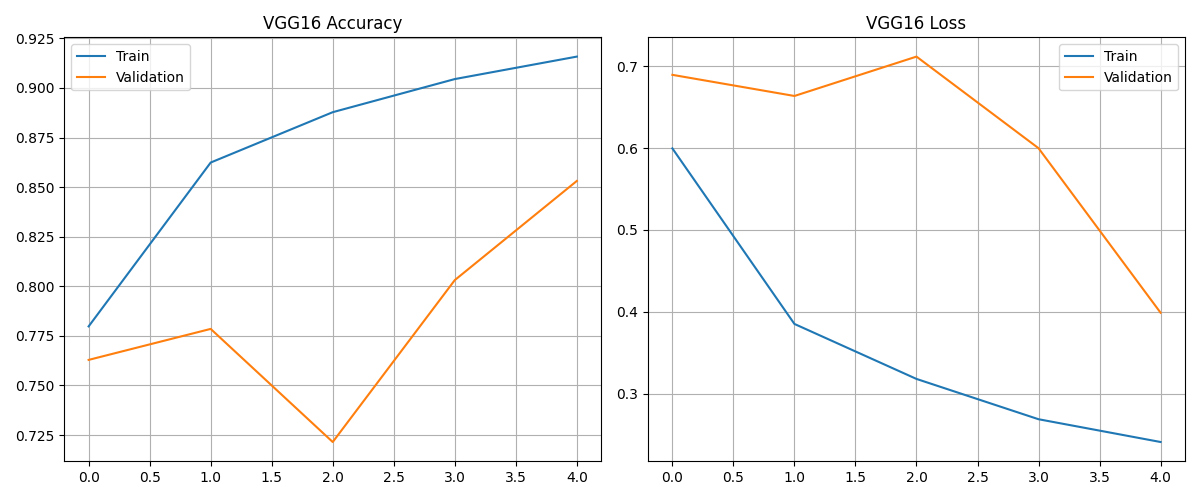
\includegraphics[width=\textwidth]{chemical_classification_models/Accuracy_Loss_Curves/VGG16.png}
  \caption{VGG16}
  \label{fig:curve_vgg}
\end{subfigure}
\hfill
\begin{subfigure}{0.48\textwidth}
  \centering
  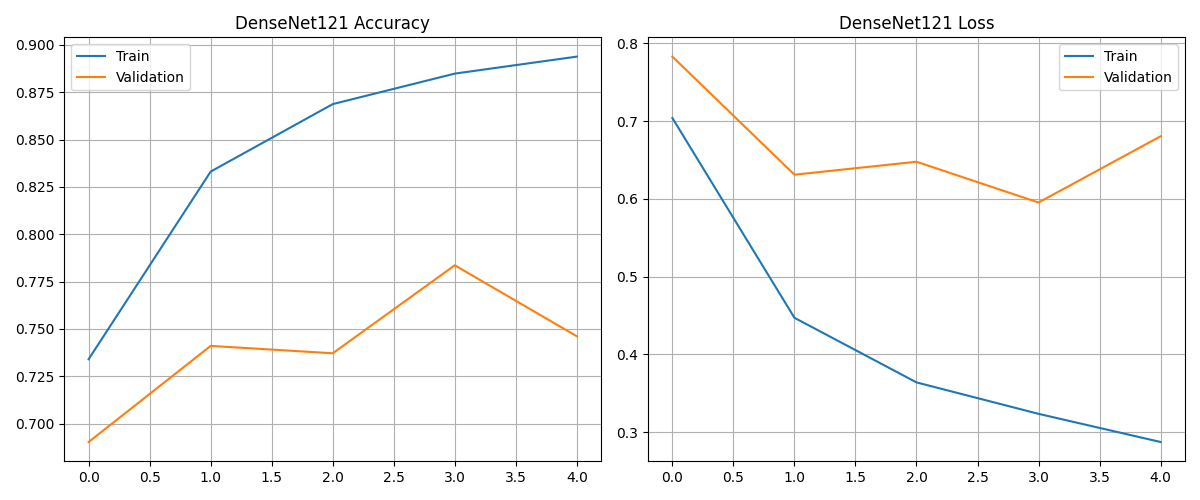
\includegraphics[width=\textwidth]{chemical_classification_models/Accuracy_Loss_Curves/DenseNet121.png}
  \caption{DenseNet121}
  \label{fig:curve_dense}
\end{subfigure}

\vspace{0.4cm}

\begin{subfigure}{0.48\textwidth}
  \centering
  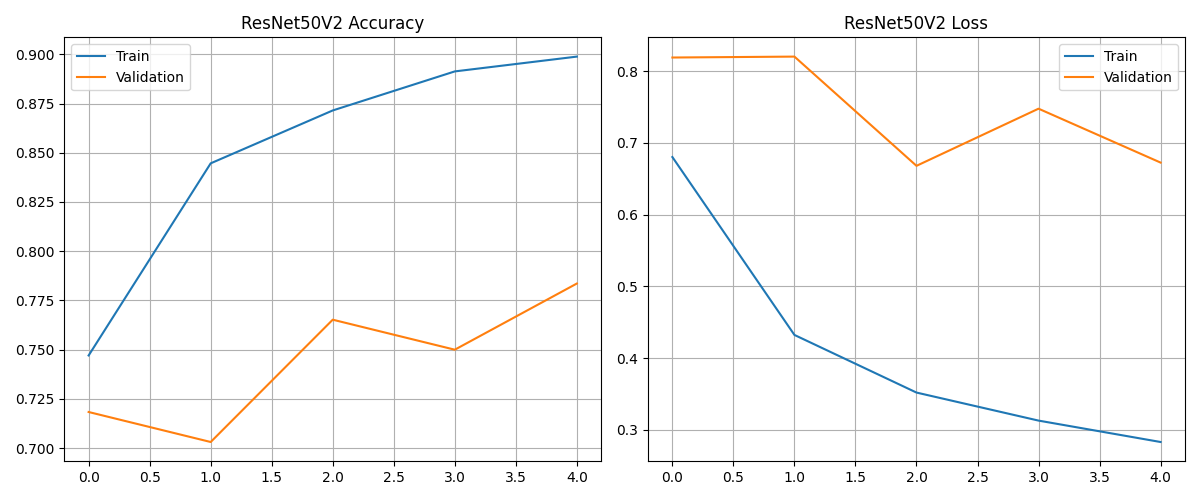
\includegraphics[width=\textwidth]{chemical_classification_models/Accuracy_Loss_Curves/ResNet50V2.png}
  \caption{ResNet50V2}
  \label{fig:curve_resnet}
\end{subfigure}
\hfill
\begin{subfigure}{0.48\textwidth}
  \centering
  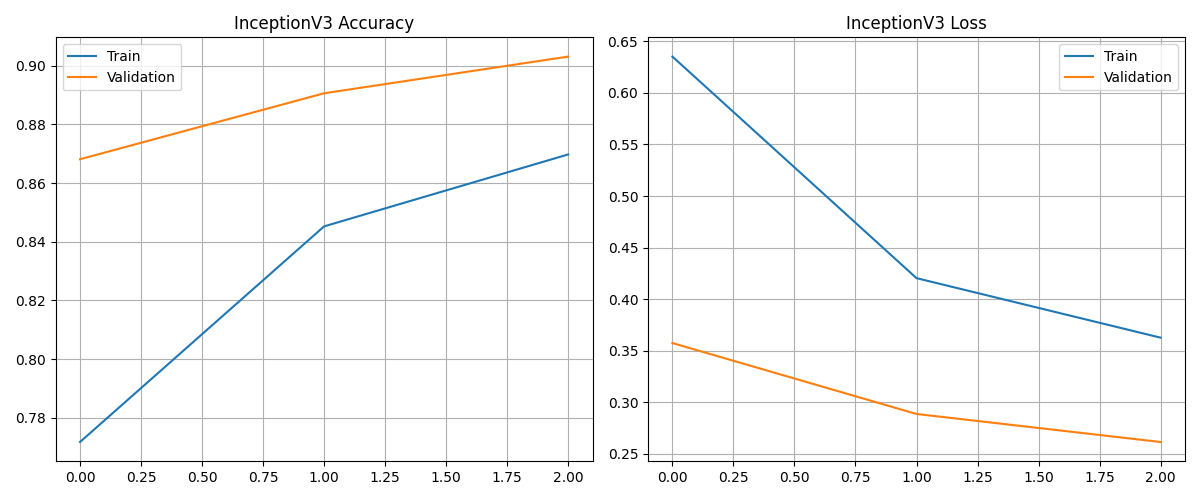
\includegraphics[width=\textwidth]{chemical_classification_models/Accuracy_Loss_Curves/InceptionV3.png}
  \caption{InceptionV3}
  \label{fig:curve_inception}
\end{subfigure}
\caption{Training and Validation Accuracy/Loss Curves --- VGG16, DenseNet121, ResNet50V2, InceptionV3}
\label{fig:accuracy_loss_curves_g1}
\end{figure}

\begin{figure}[H]
\centering
\begin{subfigure}{0.48\textwidth}
  \centering
  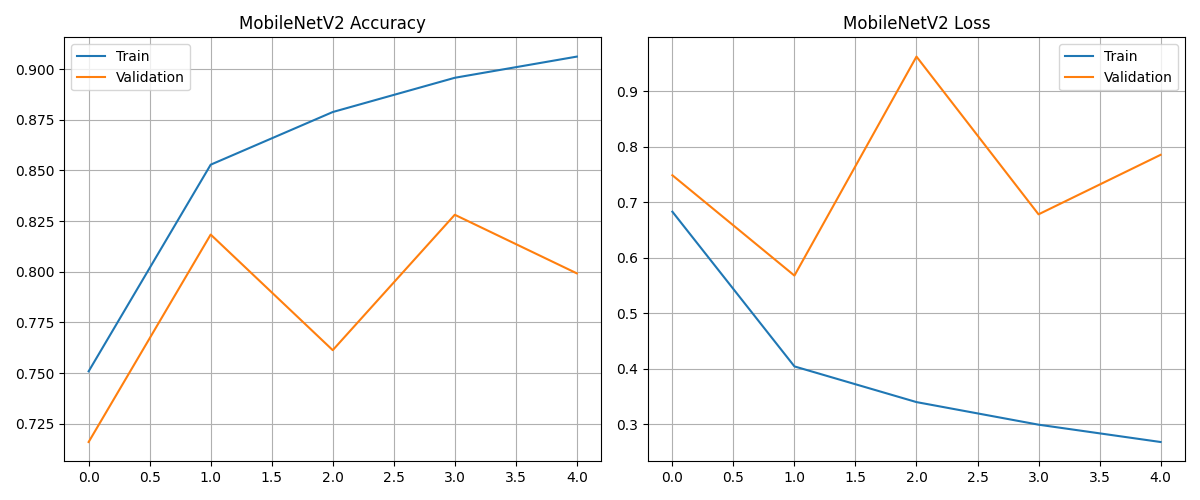
\includegraphics[width=\textwidth]{chemical_classification_models/Accuracy_Loss_Curves/MobileNetV2.png}
  \caption{MobileNetV2}
  \label{fig:curve_mobile}
\end{subfigure}
\hfill
\begin{subfigure}{0.48\textwidth}
  \centering
  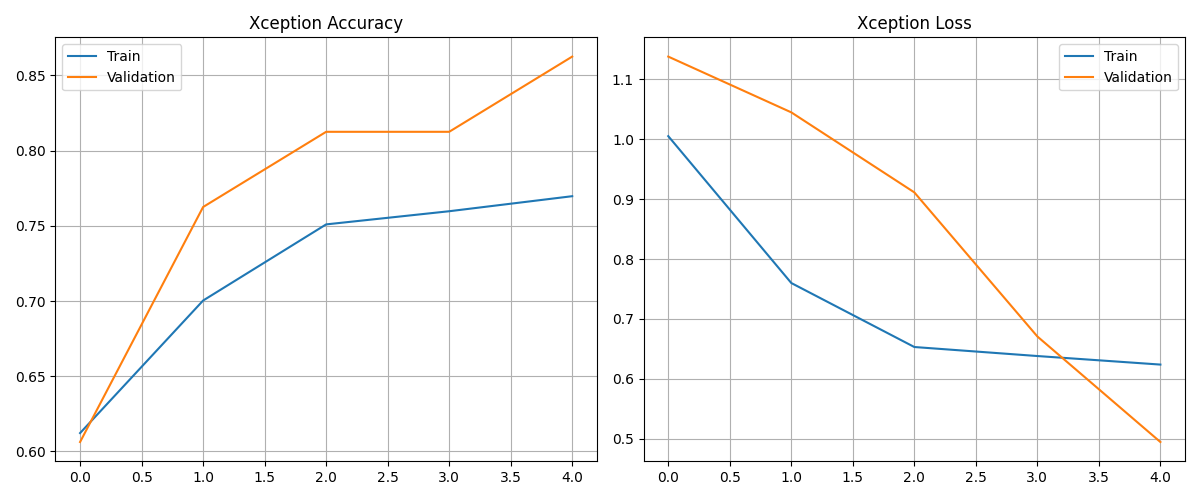
\includegraphics[width=\textwidth]{chemical_classification_models/Accuracy_Loss_Curves/Xception.png}
  \caption{Xception}
  \label{fig:curve_xception}
\end{subfigure}

\vspace{0.4cm}

\begin{subfigure}{0.48\textwidth}
  \centering
  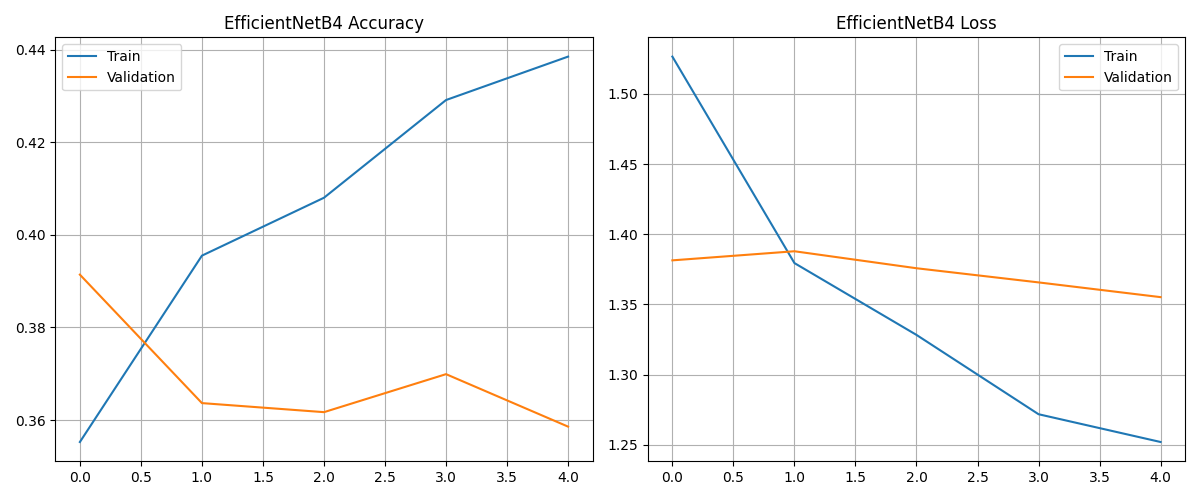
\includegraphics[width=\textwidth]{chemical_classification_models/Accuracy_Loss_Curves/EfficientNetB4.png}
  \caption{EfficientNetB4}
  \label{fig:curve_effnet}
\end{subfigure}
\hfill
\begin{subfigure}{0.48\textwidth}
  \centering
  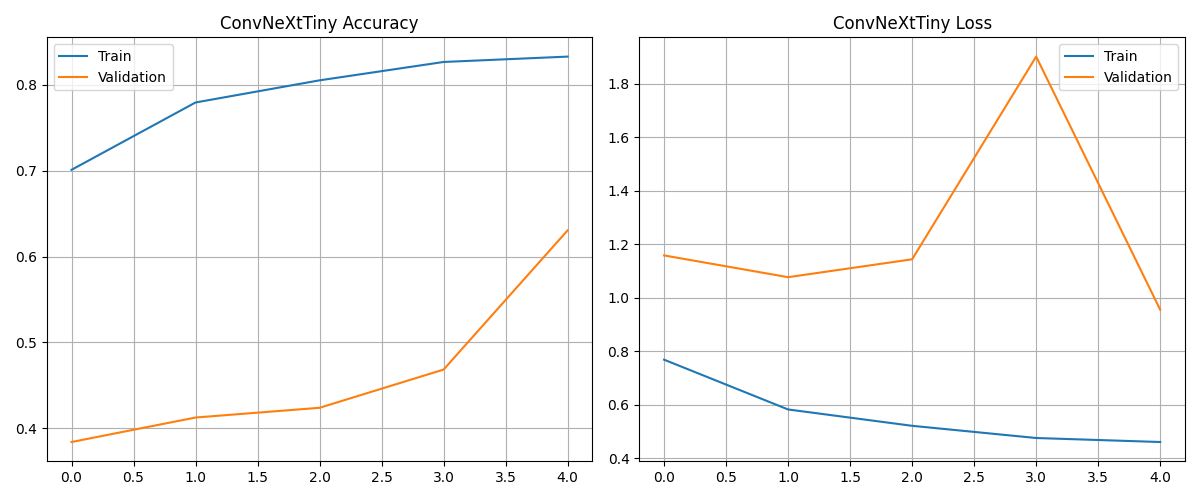
\includegraphics[width=\textwidth]{chemical_classification_models/Accuracy_Loss_Curves/ConvNeXtTiny.png}
  \caption{ConvNeXtTiny}
  \label{fig:curve_convnext}
\end{subfigure}
\caption{Training and Validation Accuracy/Loss Curves --- MobileNetV2, Xception, EfficientNetB4, ConvNeXtTiny}
\label{fig:accuracy_loss_curves_g2}
\end{figure}

\begin{figure}[H]
\centering
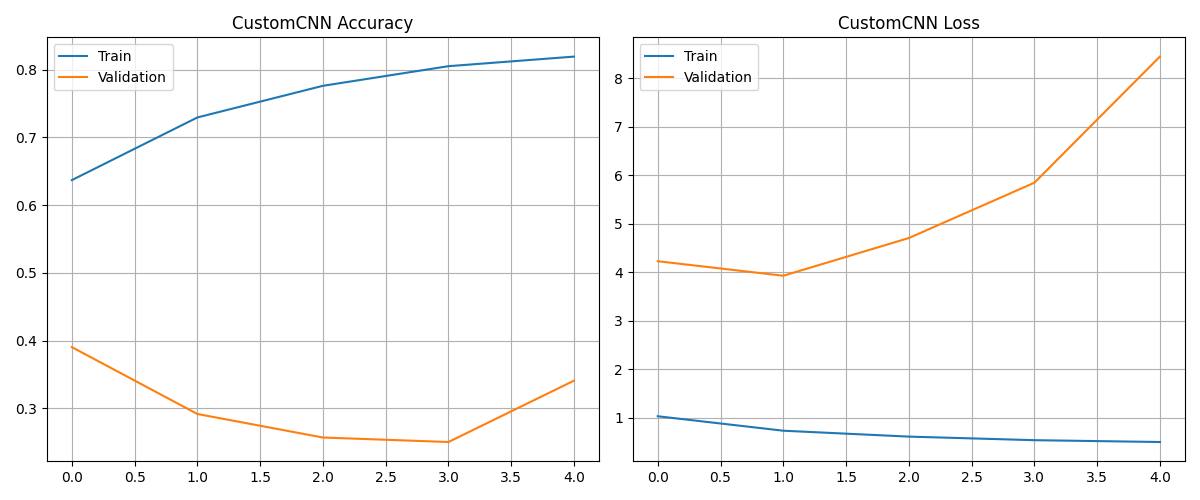
\includegraphics[width=0.66\textwidth]{chemical_classification_models/Accuracy_Loss_Curves/CustomCNN.png}
\caption{Training and Validation Accuracy/Loss Curves --- Custom CNN}
\label{fig:curve_custom}
\end{figure}

% ==============================================================
%  SECTION 10: MODEL PERFORMANCE METRICS
% ==============================================================
\section{Model Performance Metrics}

All 9 models were evaluated on the held-out test set (1,600 images). The following metrics were computed: \textbf{Accuracy}, \textbf{Precision} (weighted), \textbf{Recall} (weighted), \textbf{F1-Score} (weighted).

\begin{table}[H]
\centering
\caption{Model Performance Evaluation on Test Set (sorted by Accuracy)}
\label{tab:perf_metrics}
\rowcolors{2}{LightGray}{white}
\begin{tabular}{l c c c c}
  \toprule
  \textbf{Model} & \textbf{Accuracy} & \textbf{Precision} & \textbf{Recall} & \textbf{F1-Score} \\
  \midrule
  \rowcolor{green!12} \textbf{VGG16}       & \textbf{0.9106} & \textbf{0.9115} & \textbf{0.9106} & \textbf{0.9104} \\
  ResNet50V2     & 0.8988 & 0.8990 & 0.8988 & 0.8985 \\
  DenseNet121    & 0.8913 & 0.8912 & 0.8913 & 0.8910 \\
  InceptionV3    & 0.8863 & 0.8901 & 0.8863 & 0.8866 \\
  Xception       & 0.8088 & 0.8093 & 0.8088 & 0.8089 \\
  ConvNeXtTiny   & 0.7688 & 0.8152 & 0.7688 & 0.7763 \\
  MobileNetV2    & 0.7688 & 0.8338 & 0.7688 & 0.7552 \\
  EfficientNetB4 & 0.3938 & 0.5850 & 0.3938 & 0.3227 \\
  CustomCNN      & 0.2694 & 0.3267 & 0.2694 & 0.1504 \\
  \bottomrule
\end{tabular}
\end{table}

\begin{insightbox}[Performance Evaluation Summary]
\textbf{Best Model:} \modelname{VGG16} achieved the highest accuracy (\textbf{91.06\%}) and F1-Score (\textbf{91.04\%}).

\smallskip
\textbf{Why EfficientNetB4 underperformed (39.4\%):} Its built-in normalisation layer conflicts with the \code{rescale=1./255} pipeline --- the model expects un-normalised input, but the generator provides values already in $[0,1]$.

\smallskip
\textbf{Why Custom CNN underperformed (26.9\%):} Training a deep CNN entirely from scratch on 12,800 images is insufficient without pre-trained feature extractors. Transfer learning dominates in low-data regimes.
\end{insightbox}

% ==============================================================
%  SECTION 11: CONFUSION MATRIX
% ==============================================================
\section{Confusion Matrix \& Classification Report}

Seaborn heatmap confusion matrices were generated for all 9 models. Each cell shows the number of test images predicted as a given class for each true class (rows = true labels, columns = predicted labels).

\subsection{VGG16 Classification Report (Best Model)}

\begin{lstlisting}[numbers=none, backgroundcolor=\color{LightGray},
                   caption={VGG16 Classification Report on Test Set}]
                   precision    recall  f1-score   support

     one_molecule       0.89      0.94      0.92       400
        reactions       0.94      0.86      0.90       400
             rest       0.93      0.94      0.94       400
several_molecules       0.89      0.89      0.89       400

         accuracy                           0.91      1600
        macro avg       0.91      0.91      0.91      1600
     weighted avg       0.91      0.91      0.91      1600
\end{lstlisting}

\subsection{Confusion Matrices Grid}

\begin{figure}[H]
\centering
\begin{subfigure}{0.48\textwidth}
  \centering
  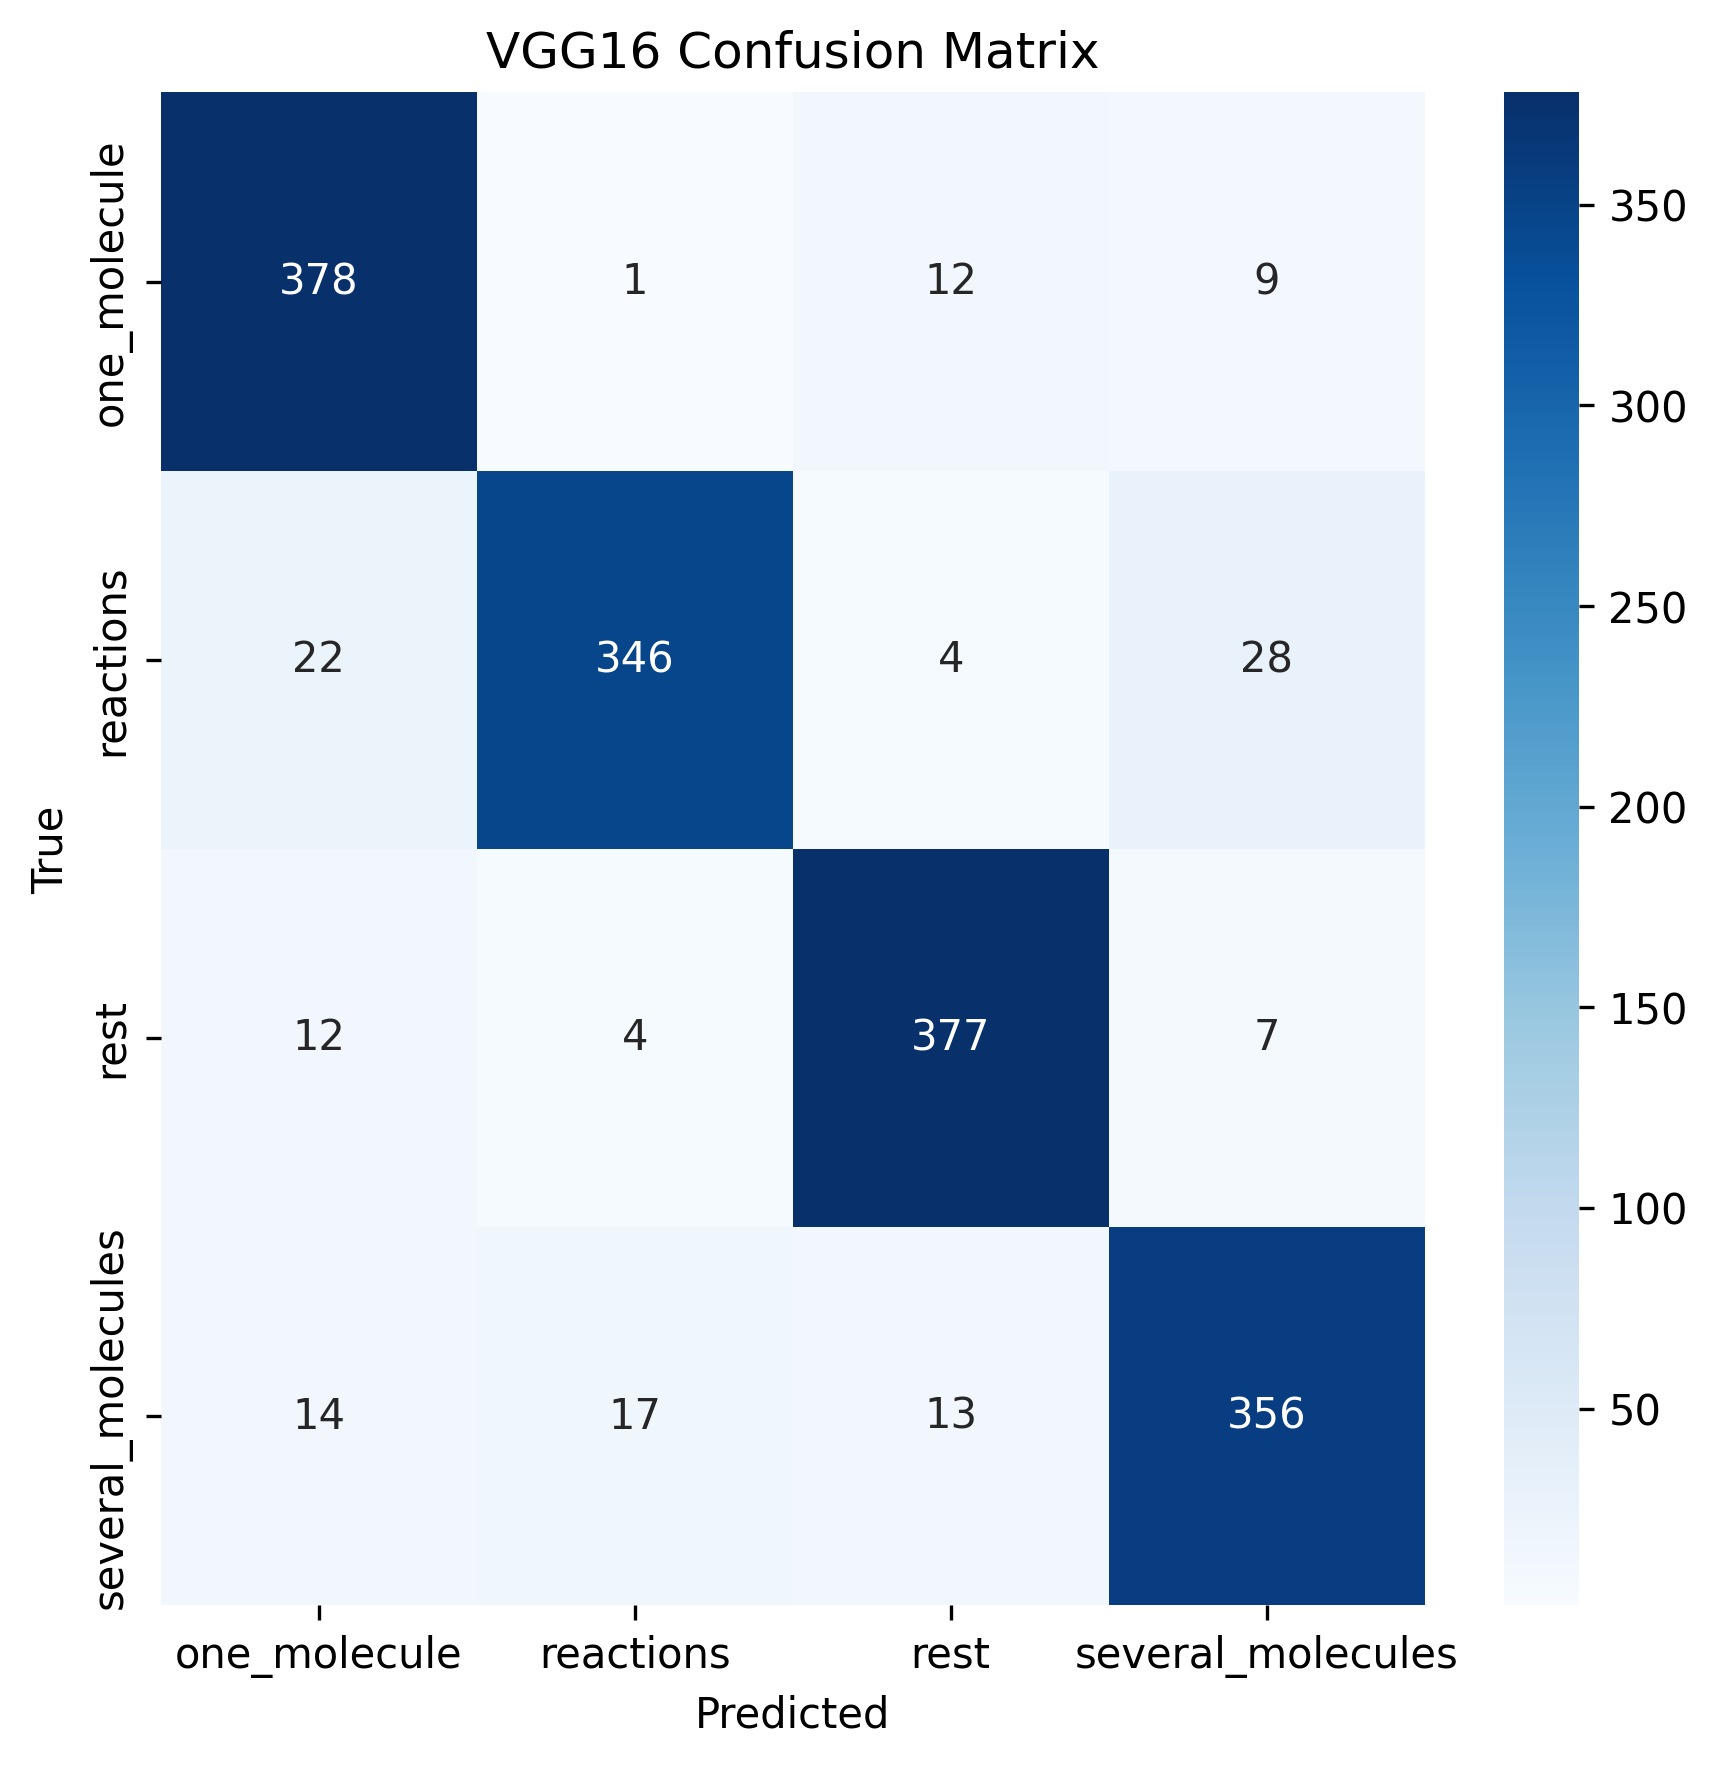
\includegraphics[width=\textwidth]{chemical_classification_models/Confusion_Matrix/VGG16_Confusion_Matrix.png}
  \caption{VGG16}
  \label{fig:cm_vgg}
\end{subfigure}
\hfill
\begin{subfigure}{0.48\textwidth}
  \centering
  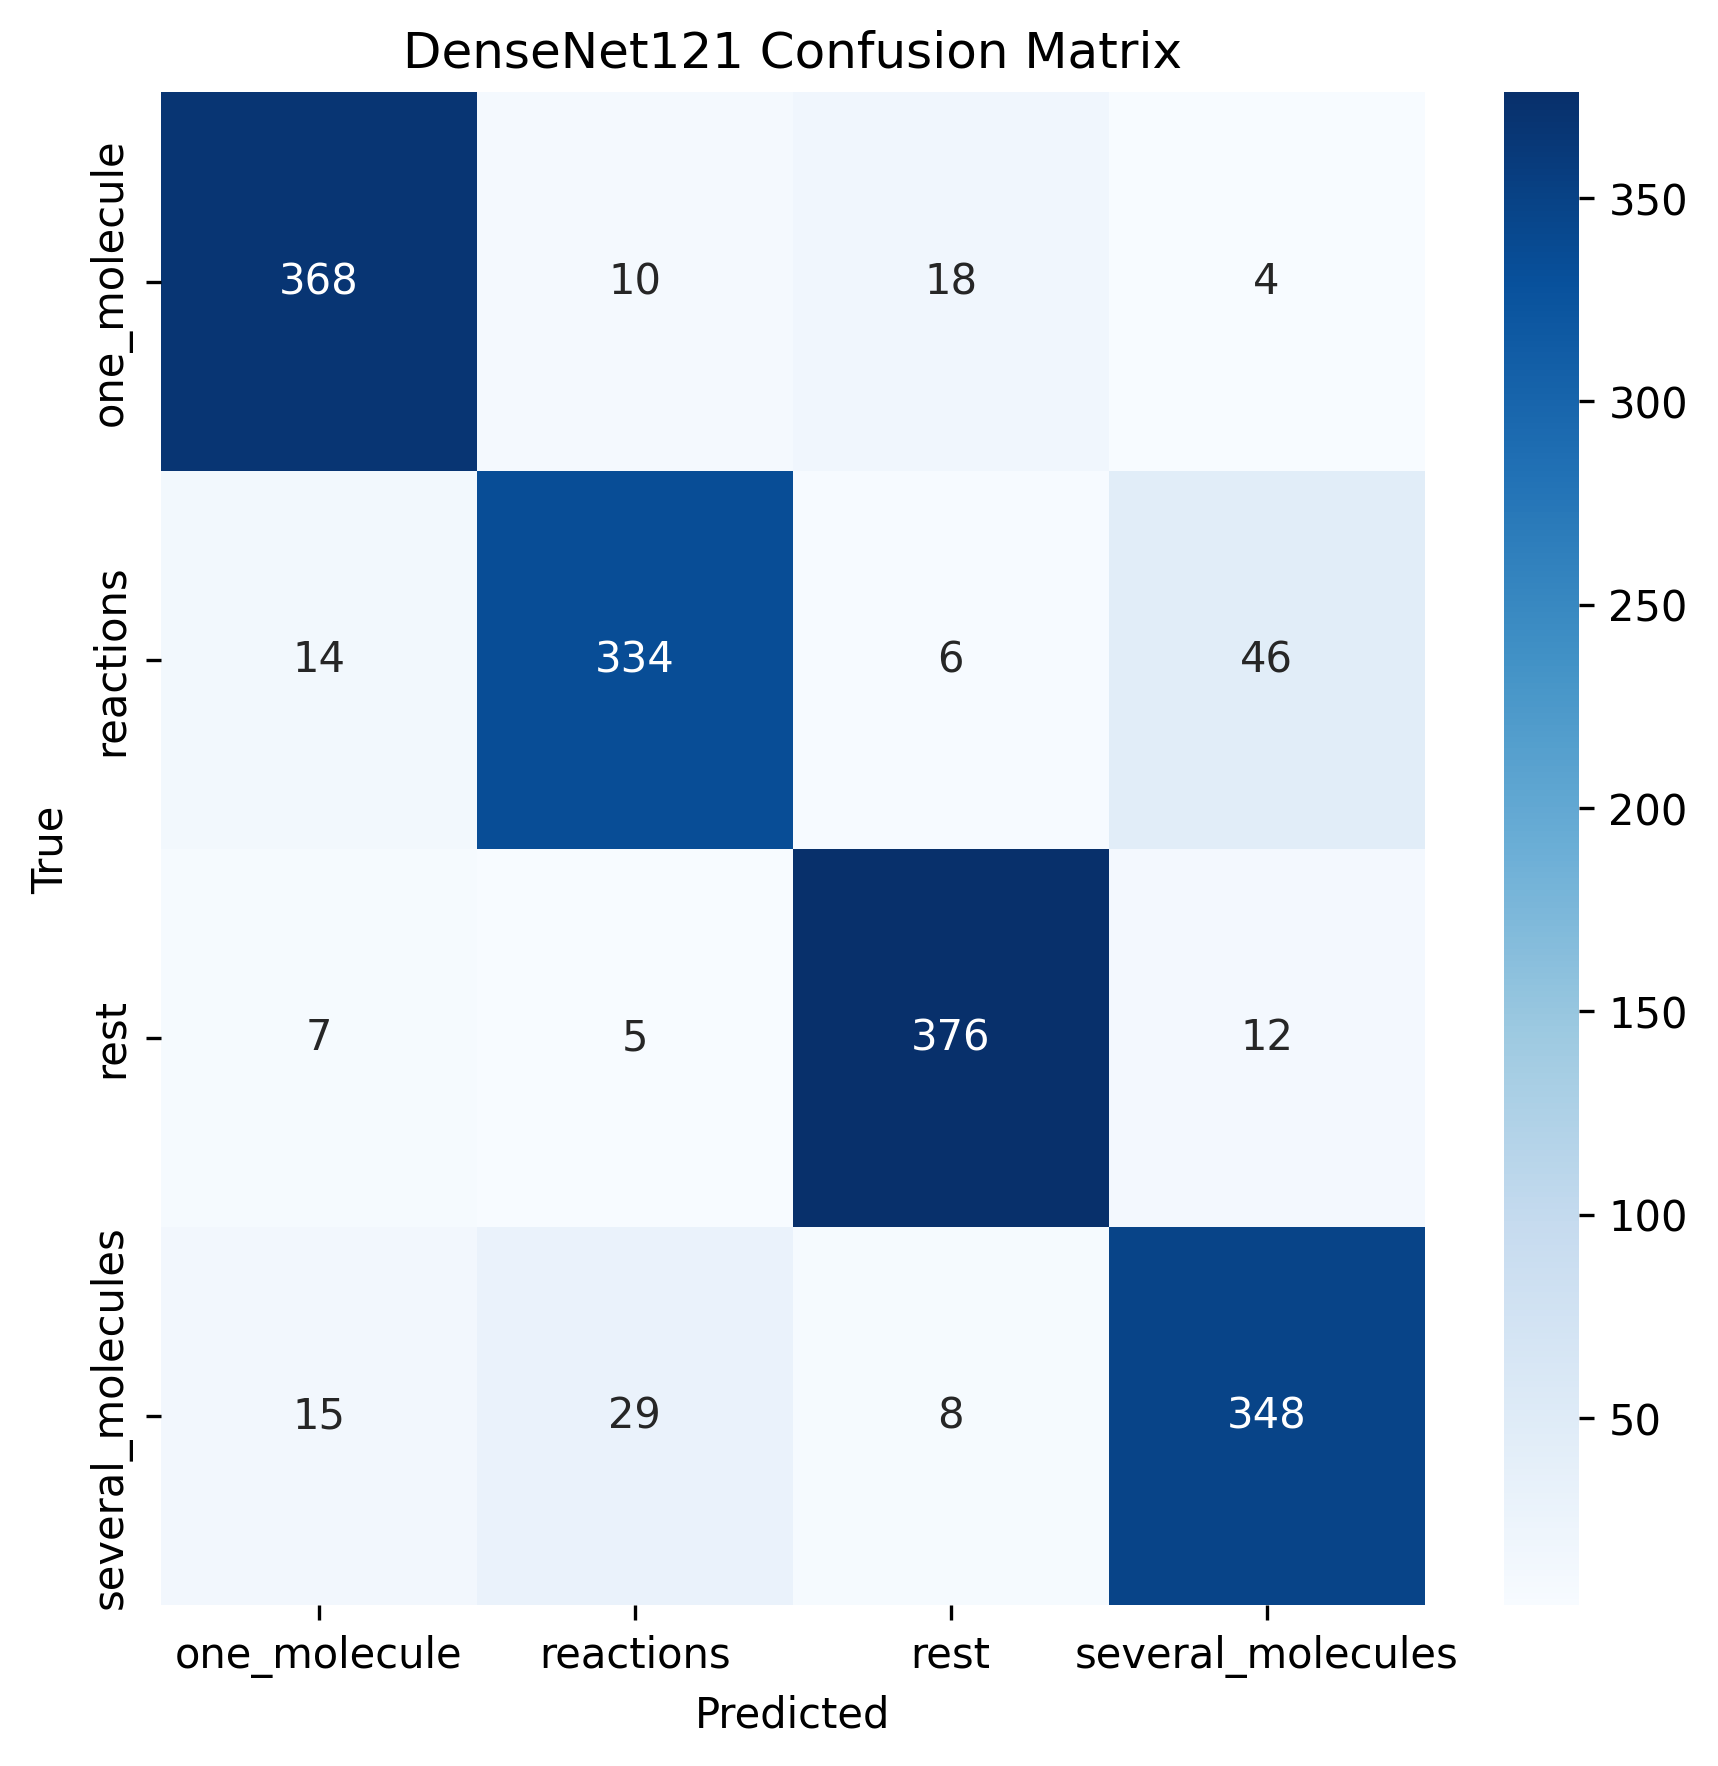
\includegraphics[width=\textwidth]{chemical_classification_models/Confusion_Matrix/DenseNet121_Confusion_Matrix.png}
  \caption{DenseNet121}
  \label{fig:cm_dense}
\end{subfigure}

\vspace{0.4cm}

\begin{subfigure}{0.48\textwidth}
  \centering
  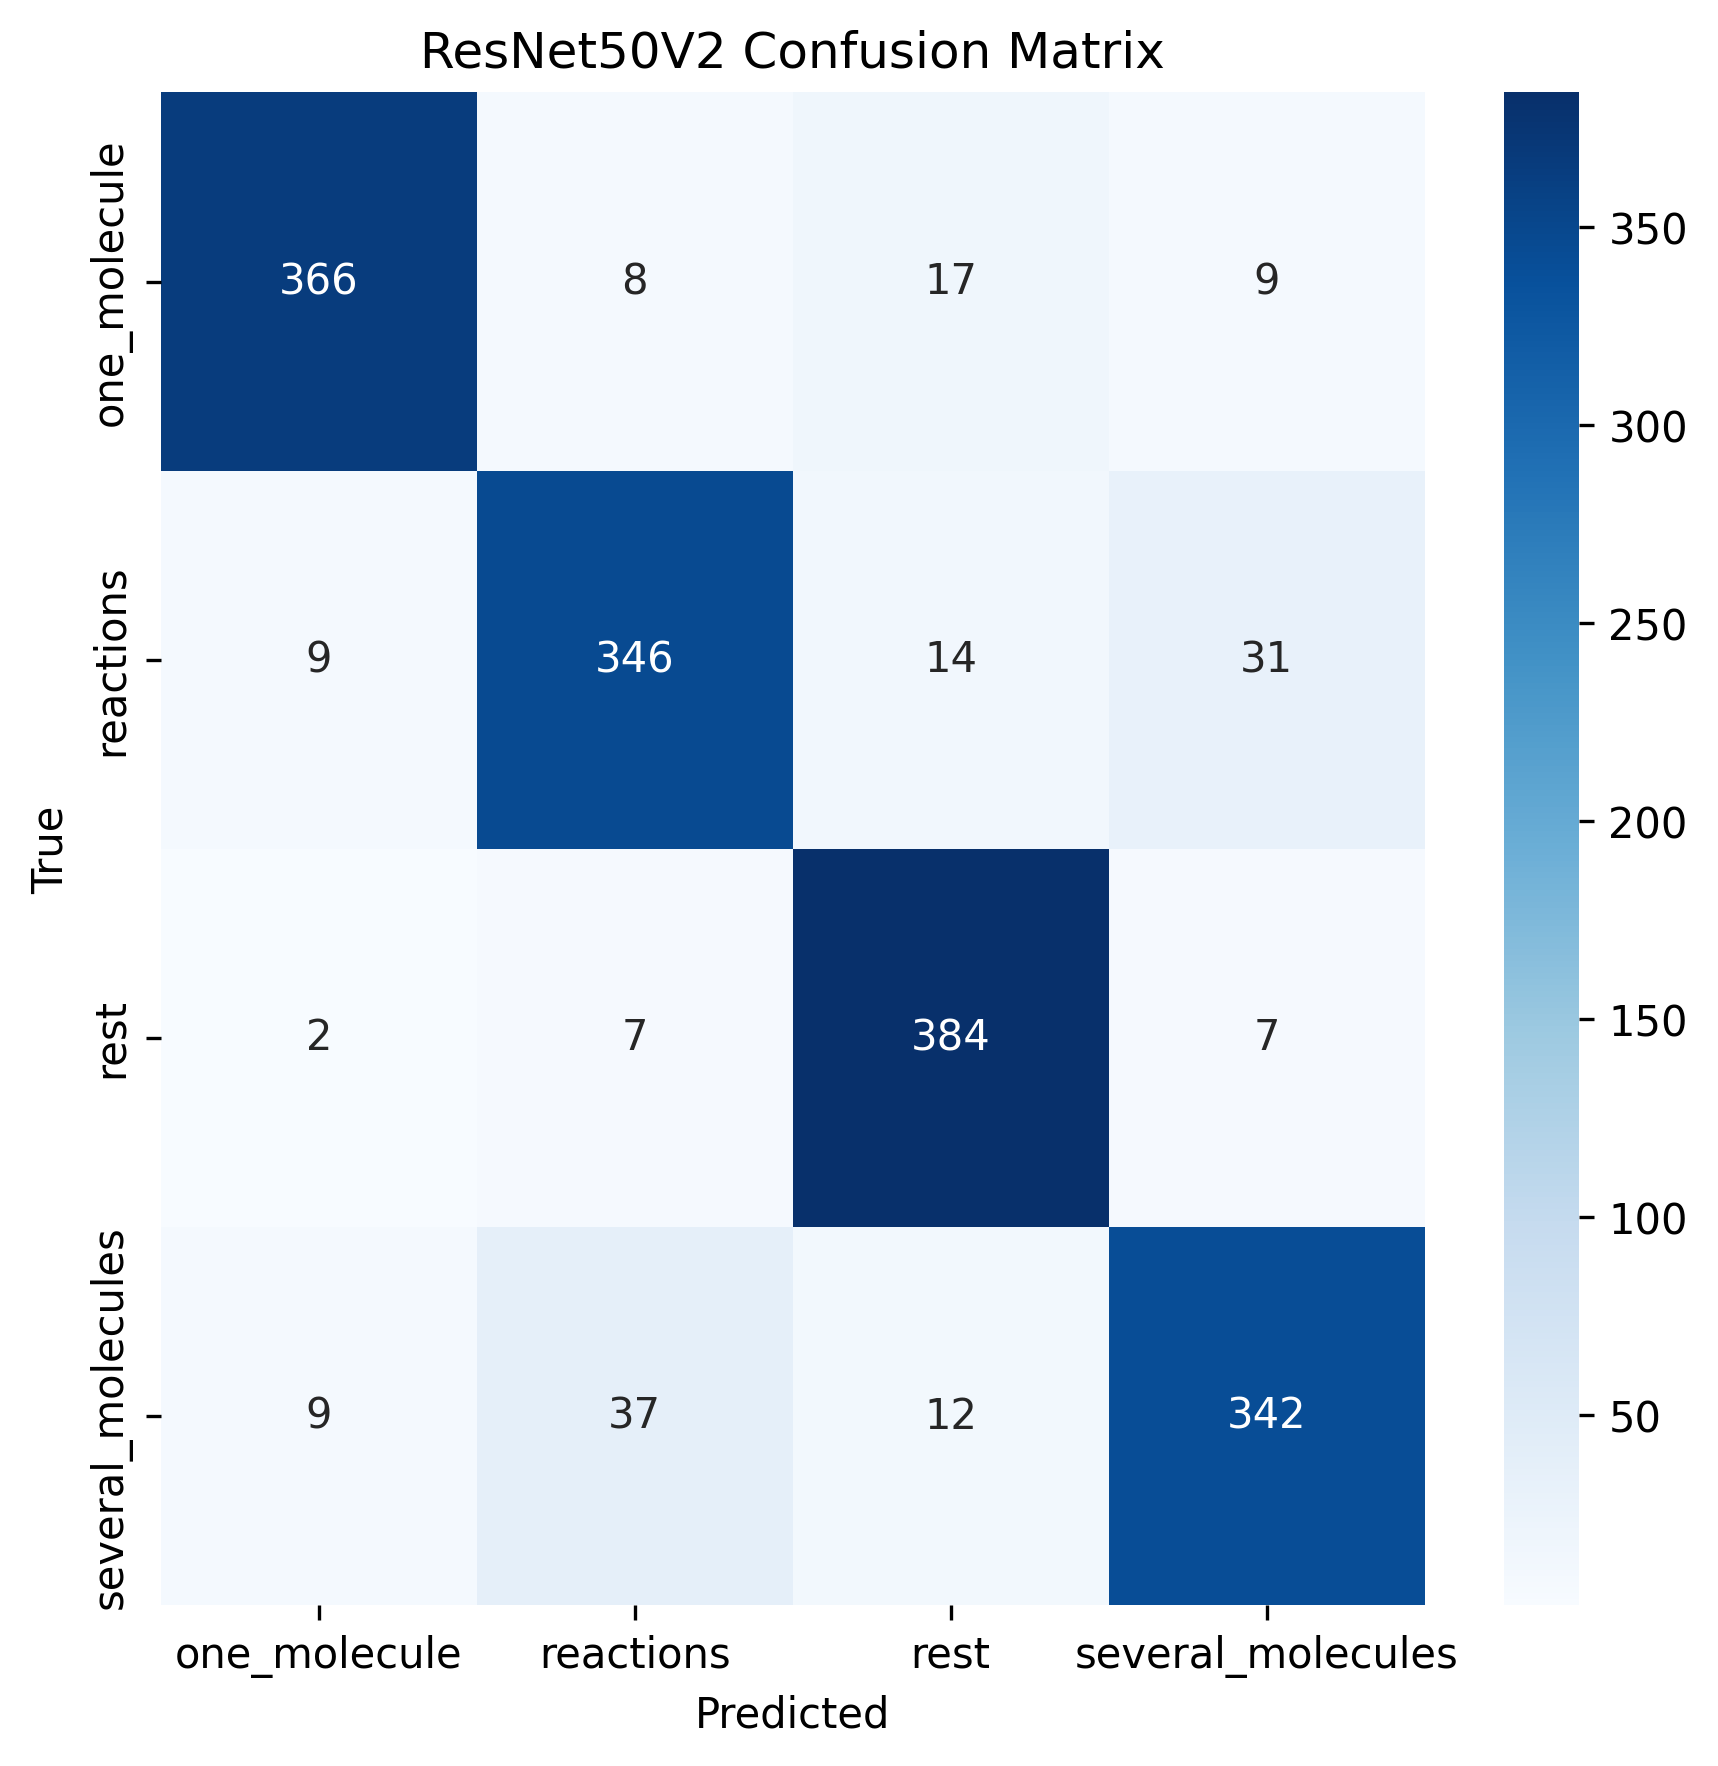
\includegraphics[width=\textwidth]{chemical_classification_models/Confusion_Matrix/ResNet50V2_Confusion_Matrix.png}
  \caption{ResNet50V2}
  \label{fig:cm_resnet}
\end{subfigure}
\hfill
\begin{subfigure}{0.48\textwidth}
  \centering
  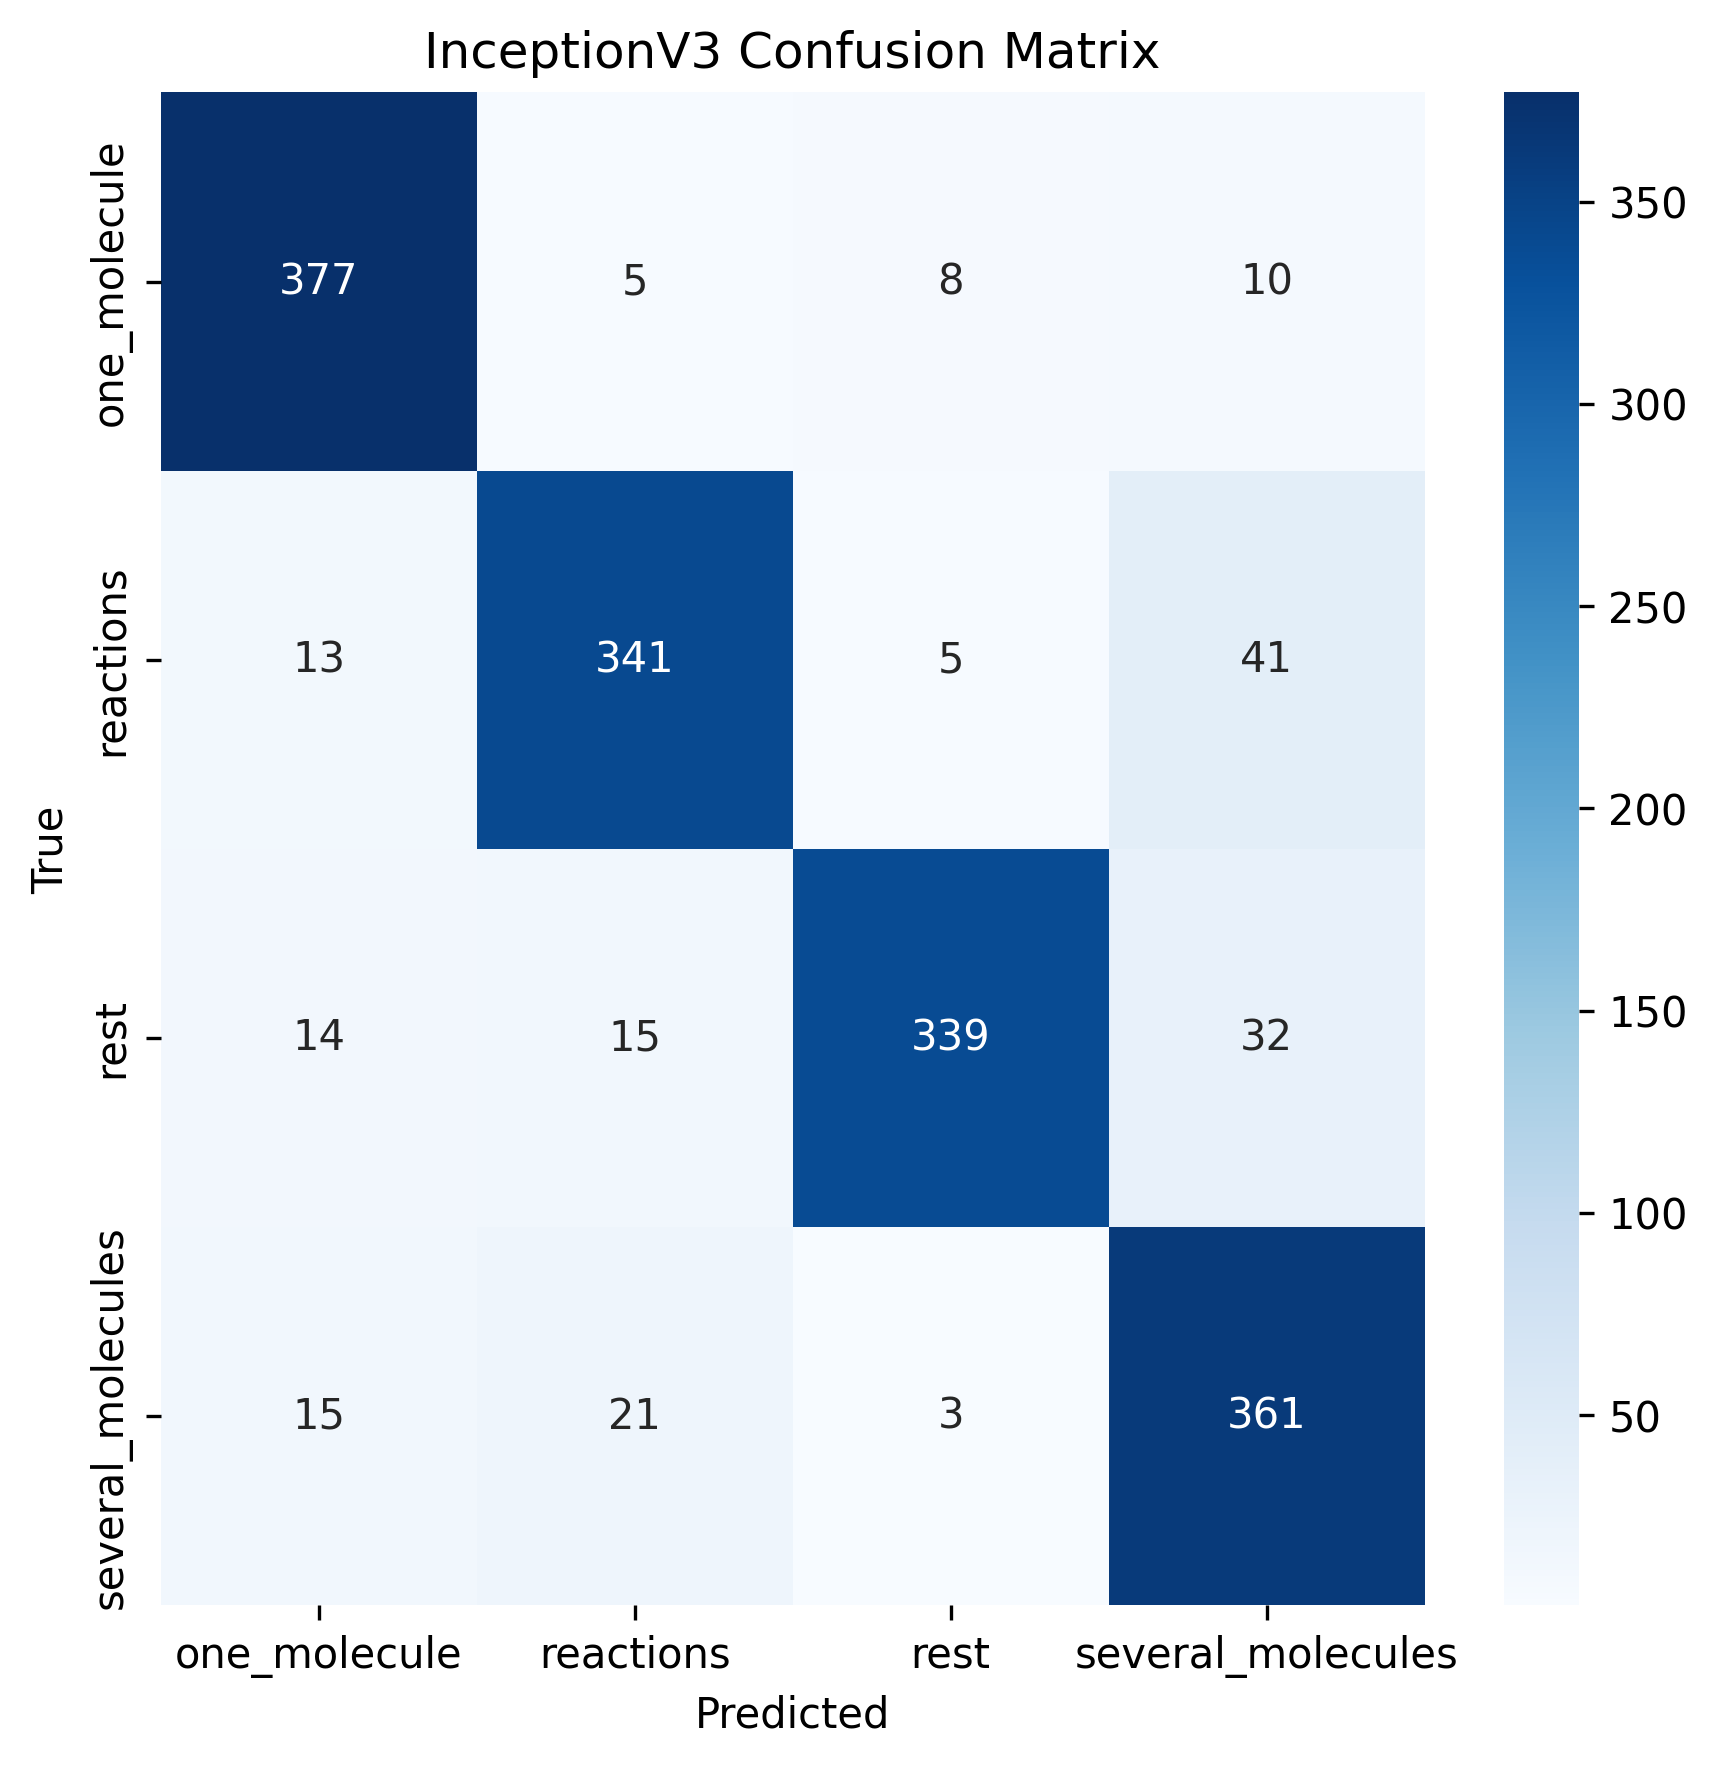
\includegraphics[width=\textwidth]{chemical_classification_models/Confusion_Matrix/InceptionV3_Confusion_Matrix.png}
  \caption{InceptionV3}
  \label{fig:cm_inception}
\end{subfigure}
\caption{Confusion Heatmaps --- VGG16, DenseNet121, ResNet50V2, InceptionV3}
\label{fig:confusion_matrices_g1}
\end{figure}

\begin{figure}[H]
\centering
\begin{subfigure}{0.48\textwidth}
  \centering
  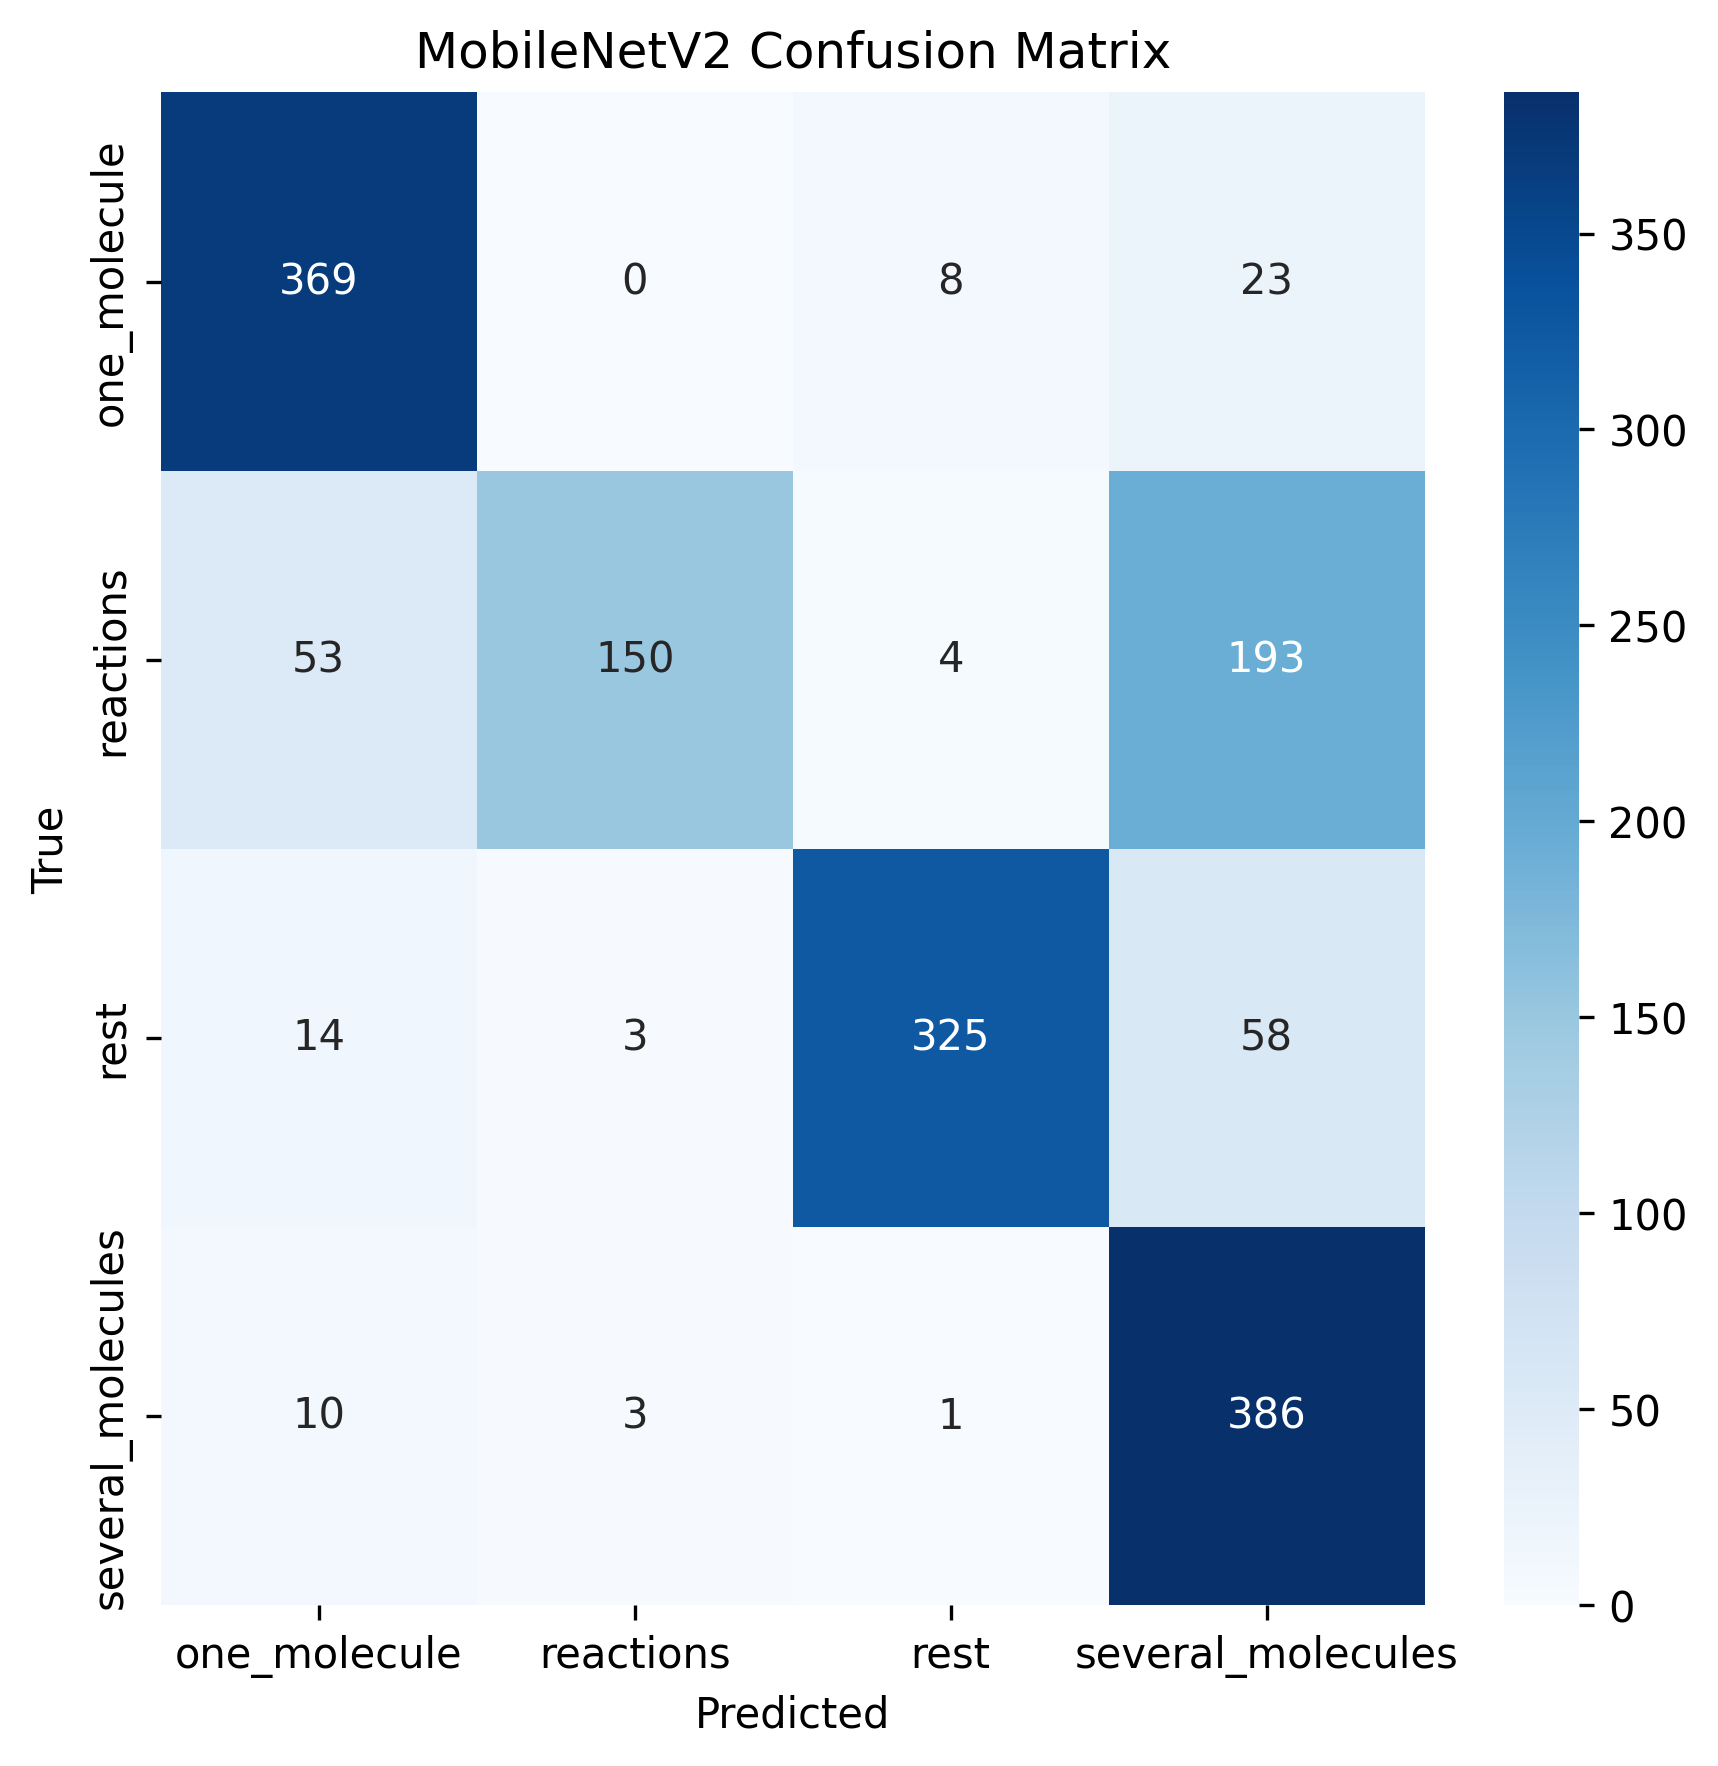
\includegraphics[width=\textwidth]{chemical_classification_models/Confusion_Matrix/MobileNetV2_Confusion_Matrix.png}
  \caption{MobileNetV2}
  \label{fig:cm_mobile}
\end{subfigure}
\hfill
\begin{subfigure}{0.48\textwidth}
  \centering
  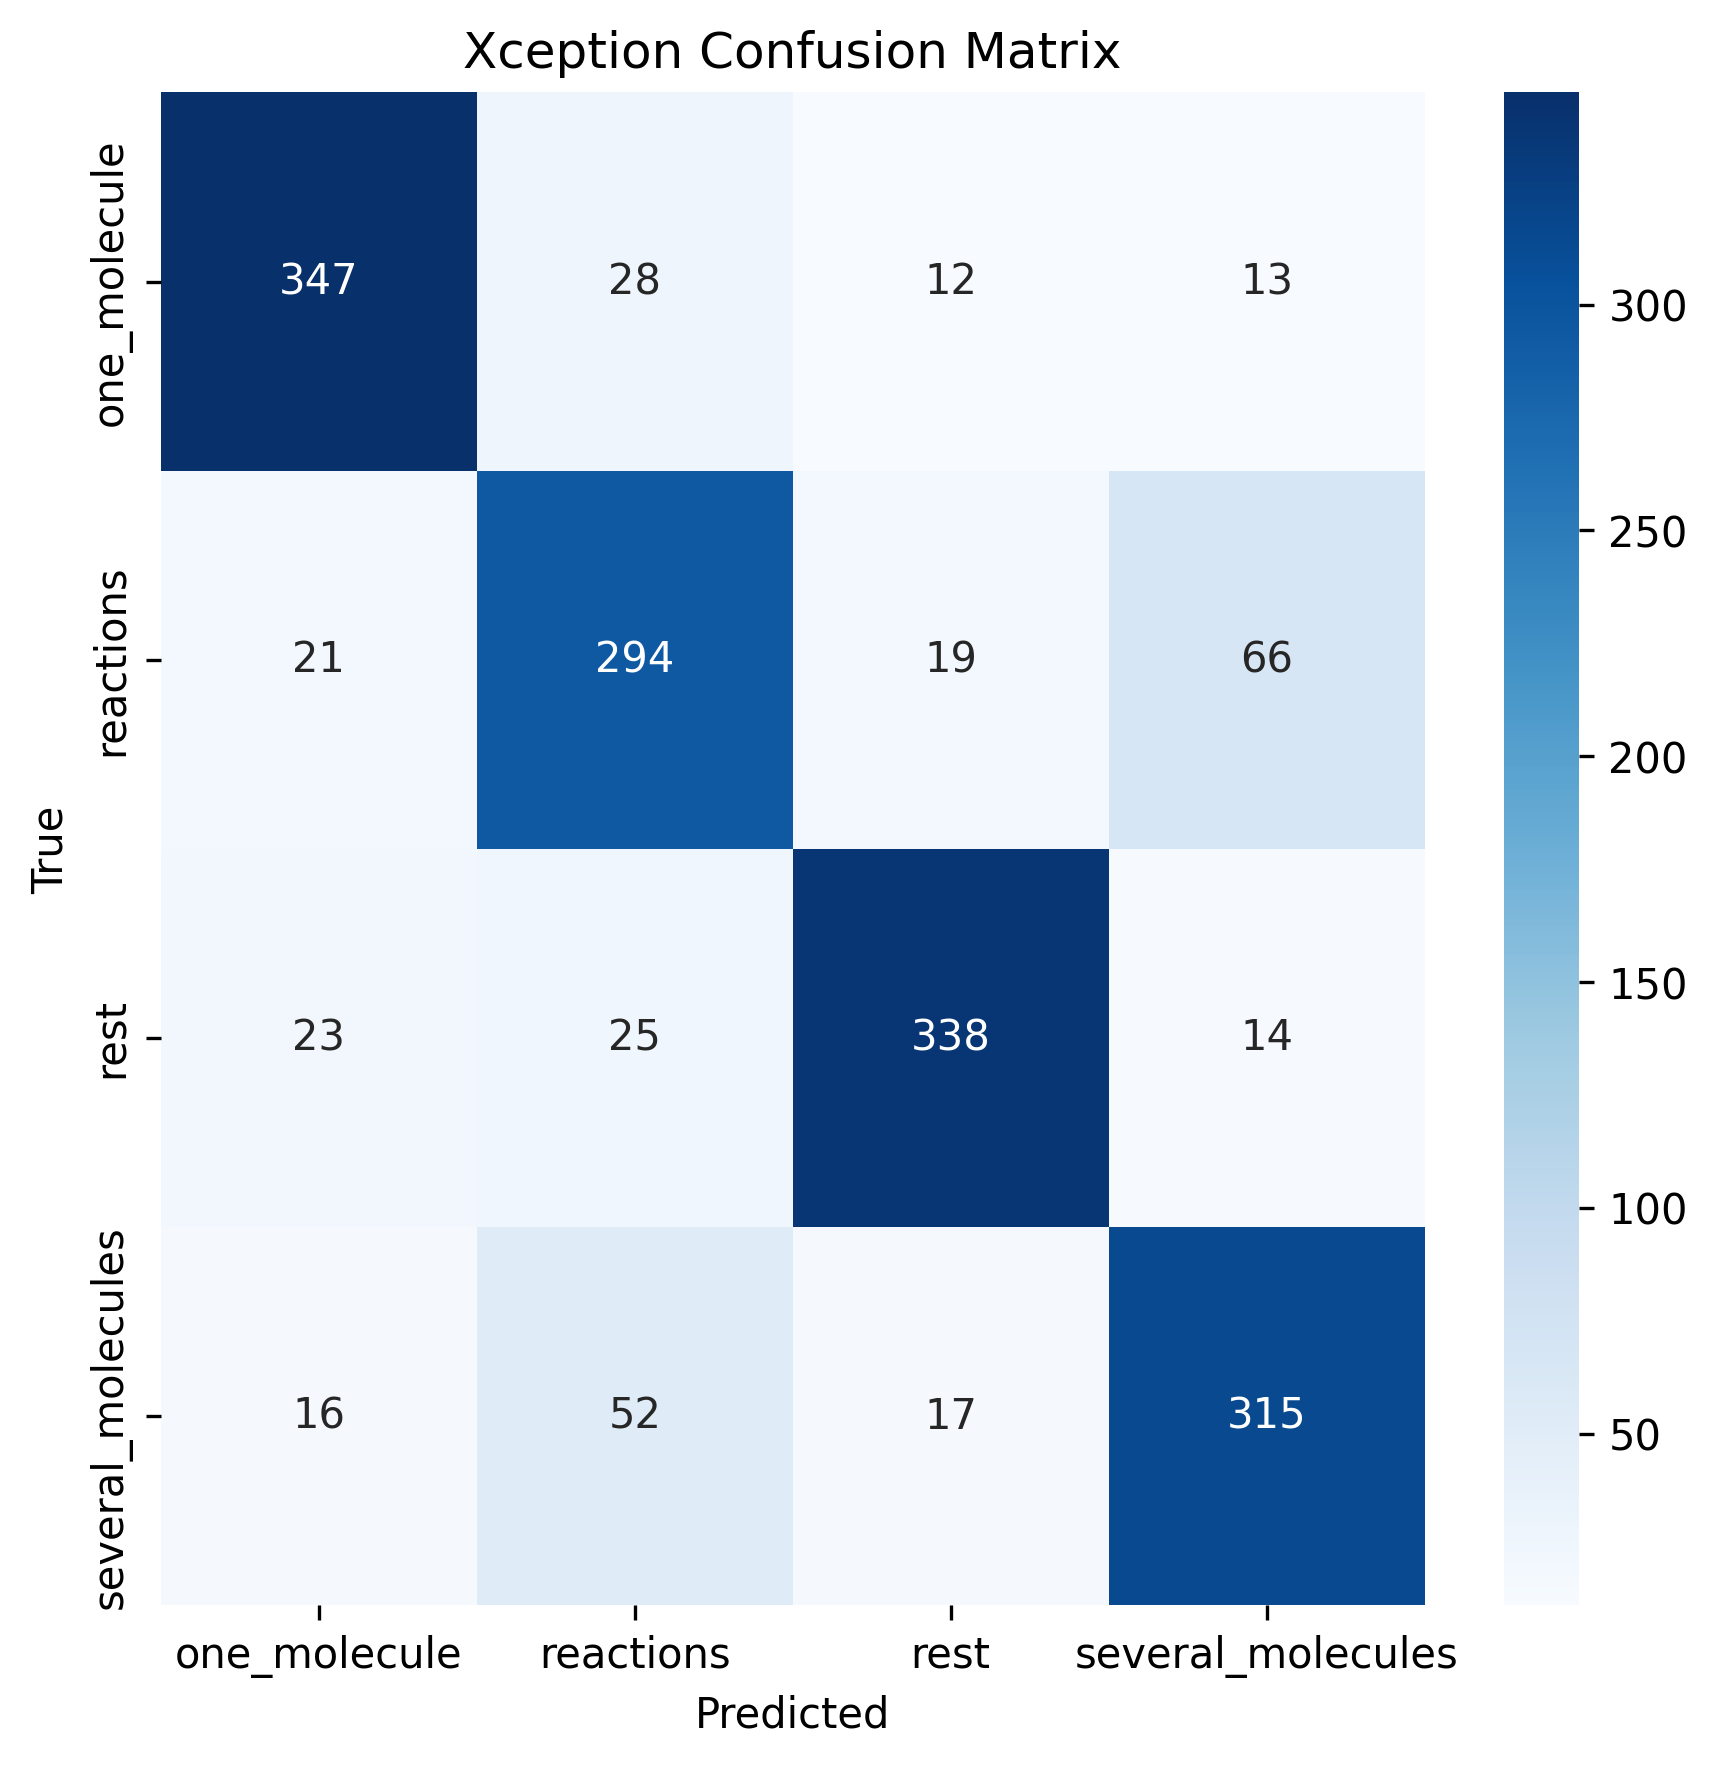
\includegraphics[width=\textwidth]{chemical_classification_models/Confusion_Matrix/Xception_Confusion_Matrix.png}
  \caption{Xception}
  \label{fig:cm_xception}
\end{subfigure}

\vspace{0.4cm}

\begin{subfigure}{0.48\textwidth}
  \centering
  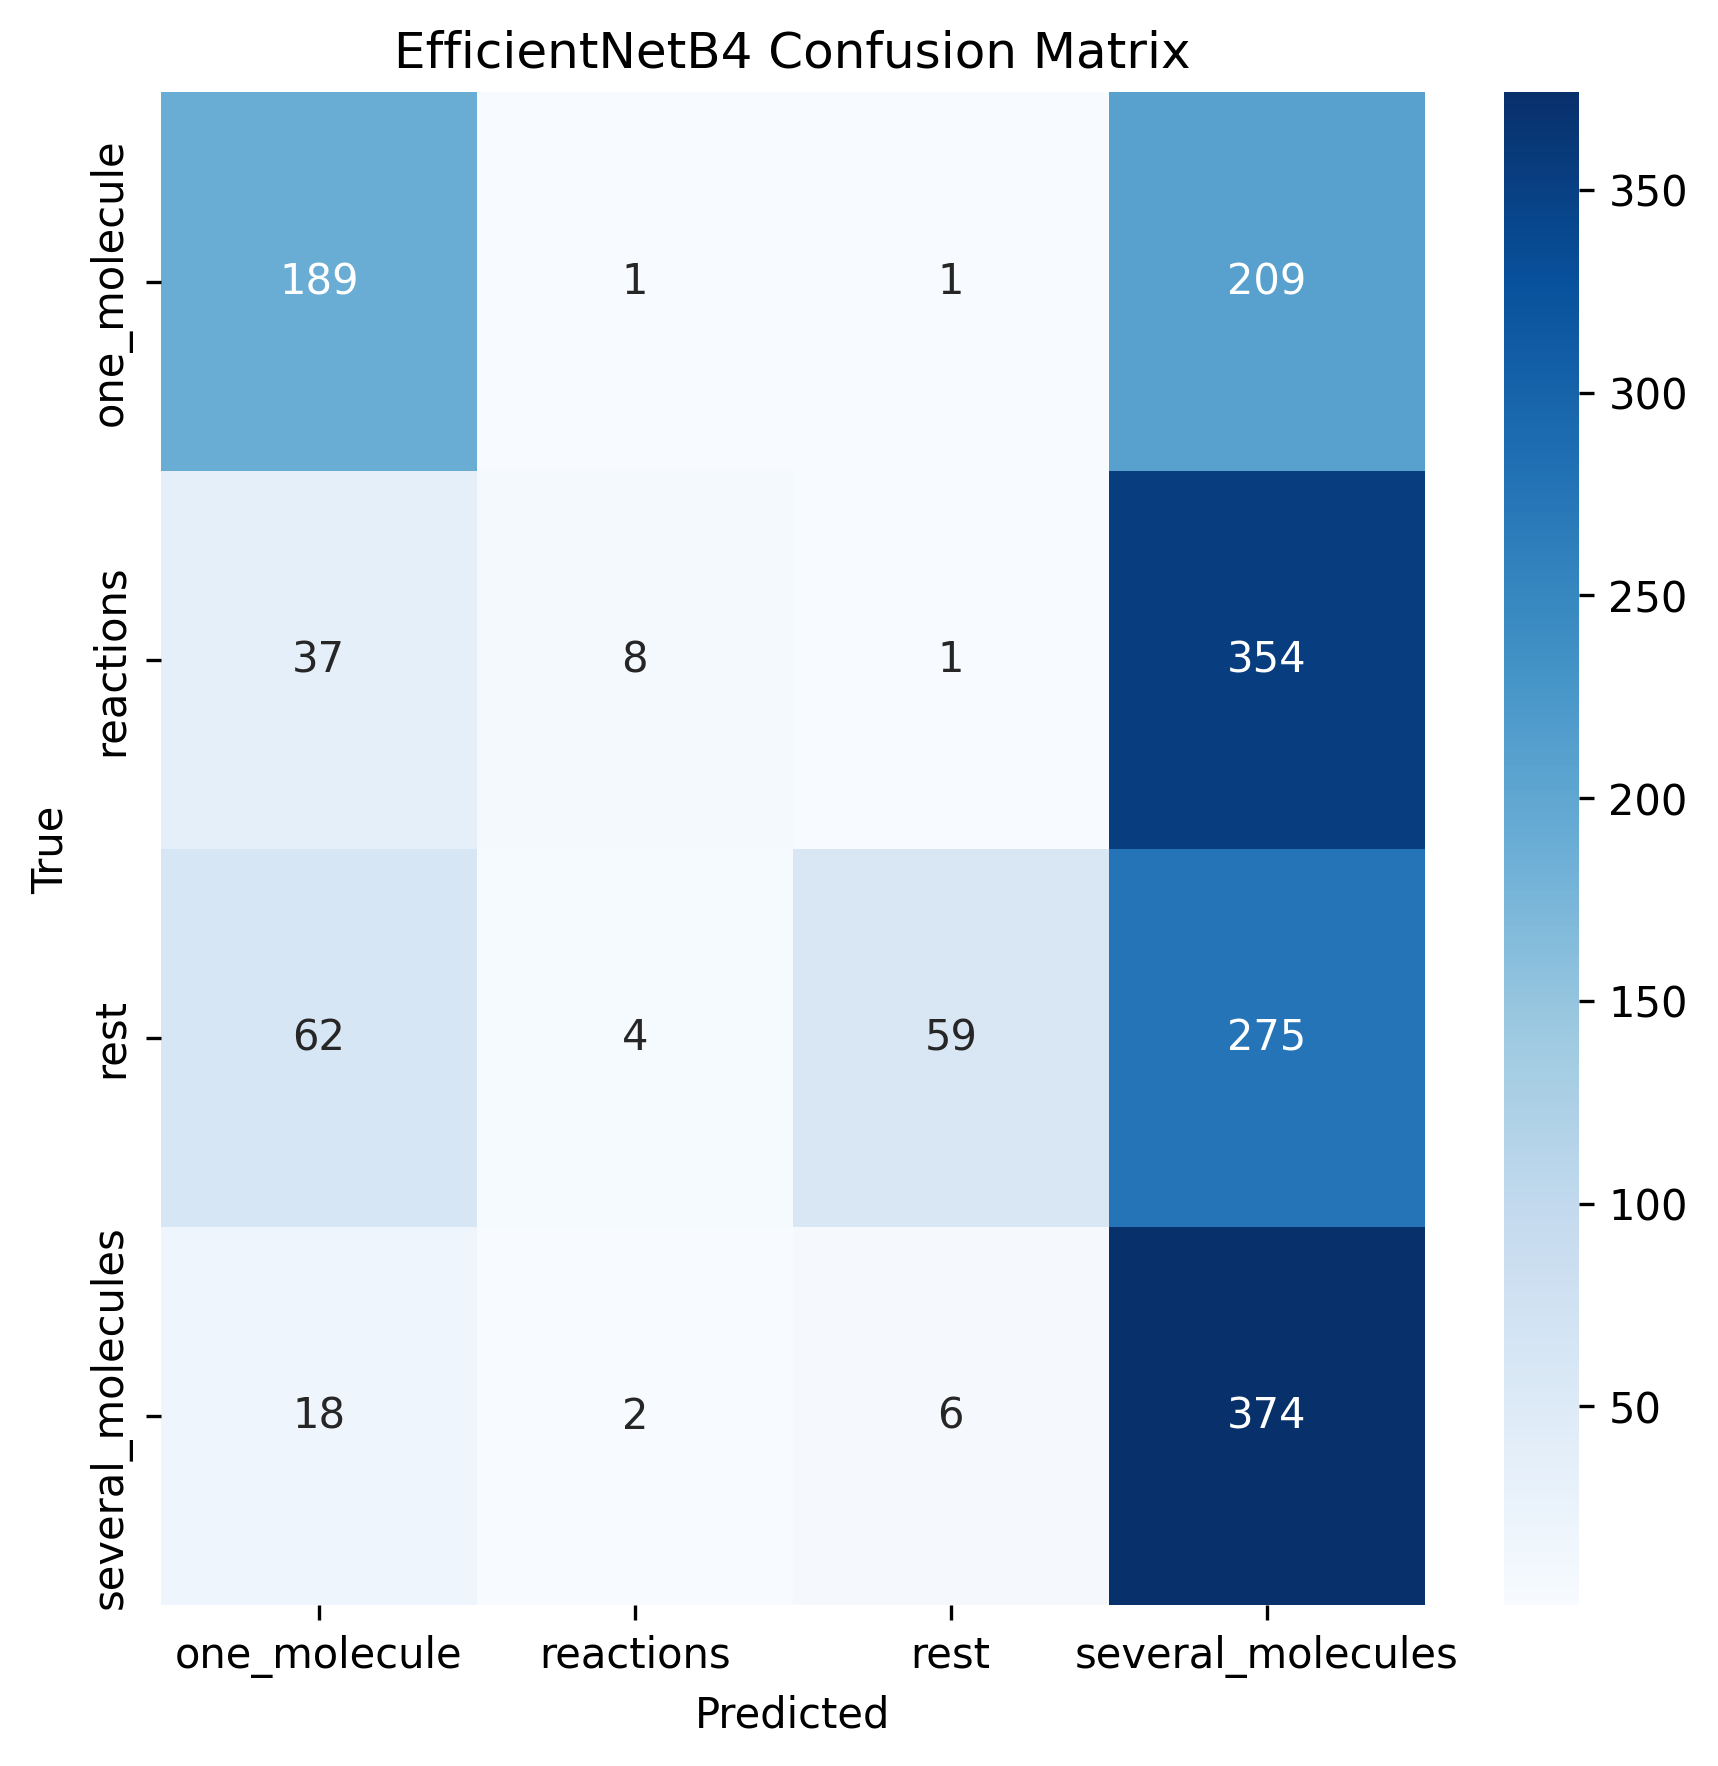
\includegraphics[width=\textwidth]{chemical_classification_models/Confusion_Matrix/EfficientNetB4_Confusion_Matrix.png}
  \caption{EfficientNetB4}
  \label{fig:cm_effnet}
\end{subfigure}
\hfill
\begin{subfigure}{0.48\textwidth}
  \centering
  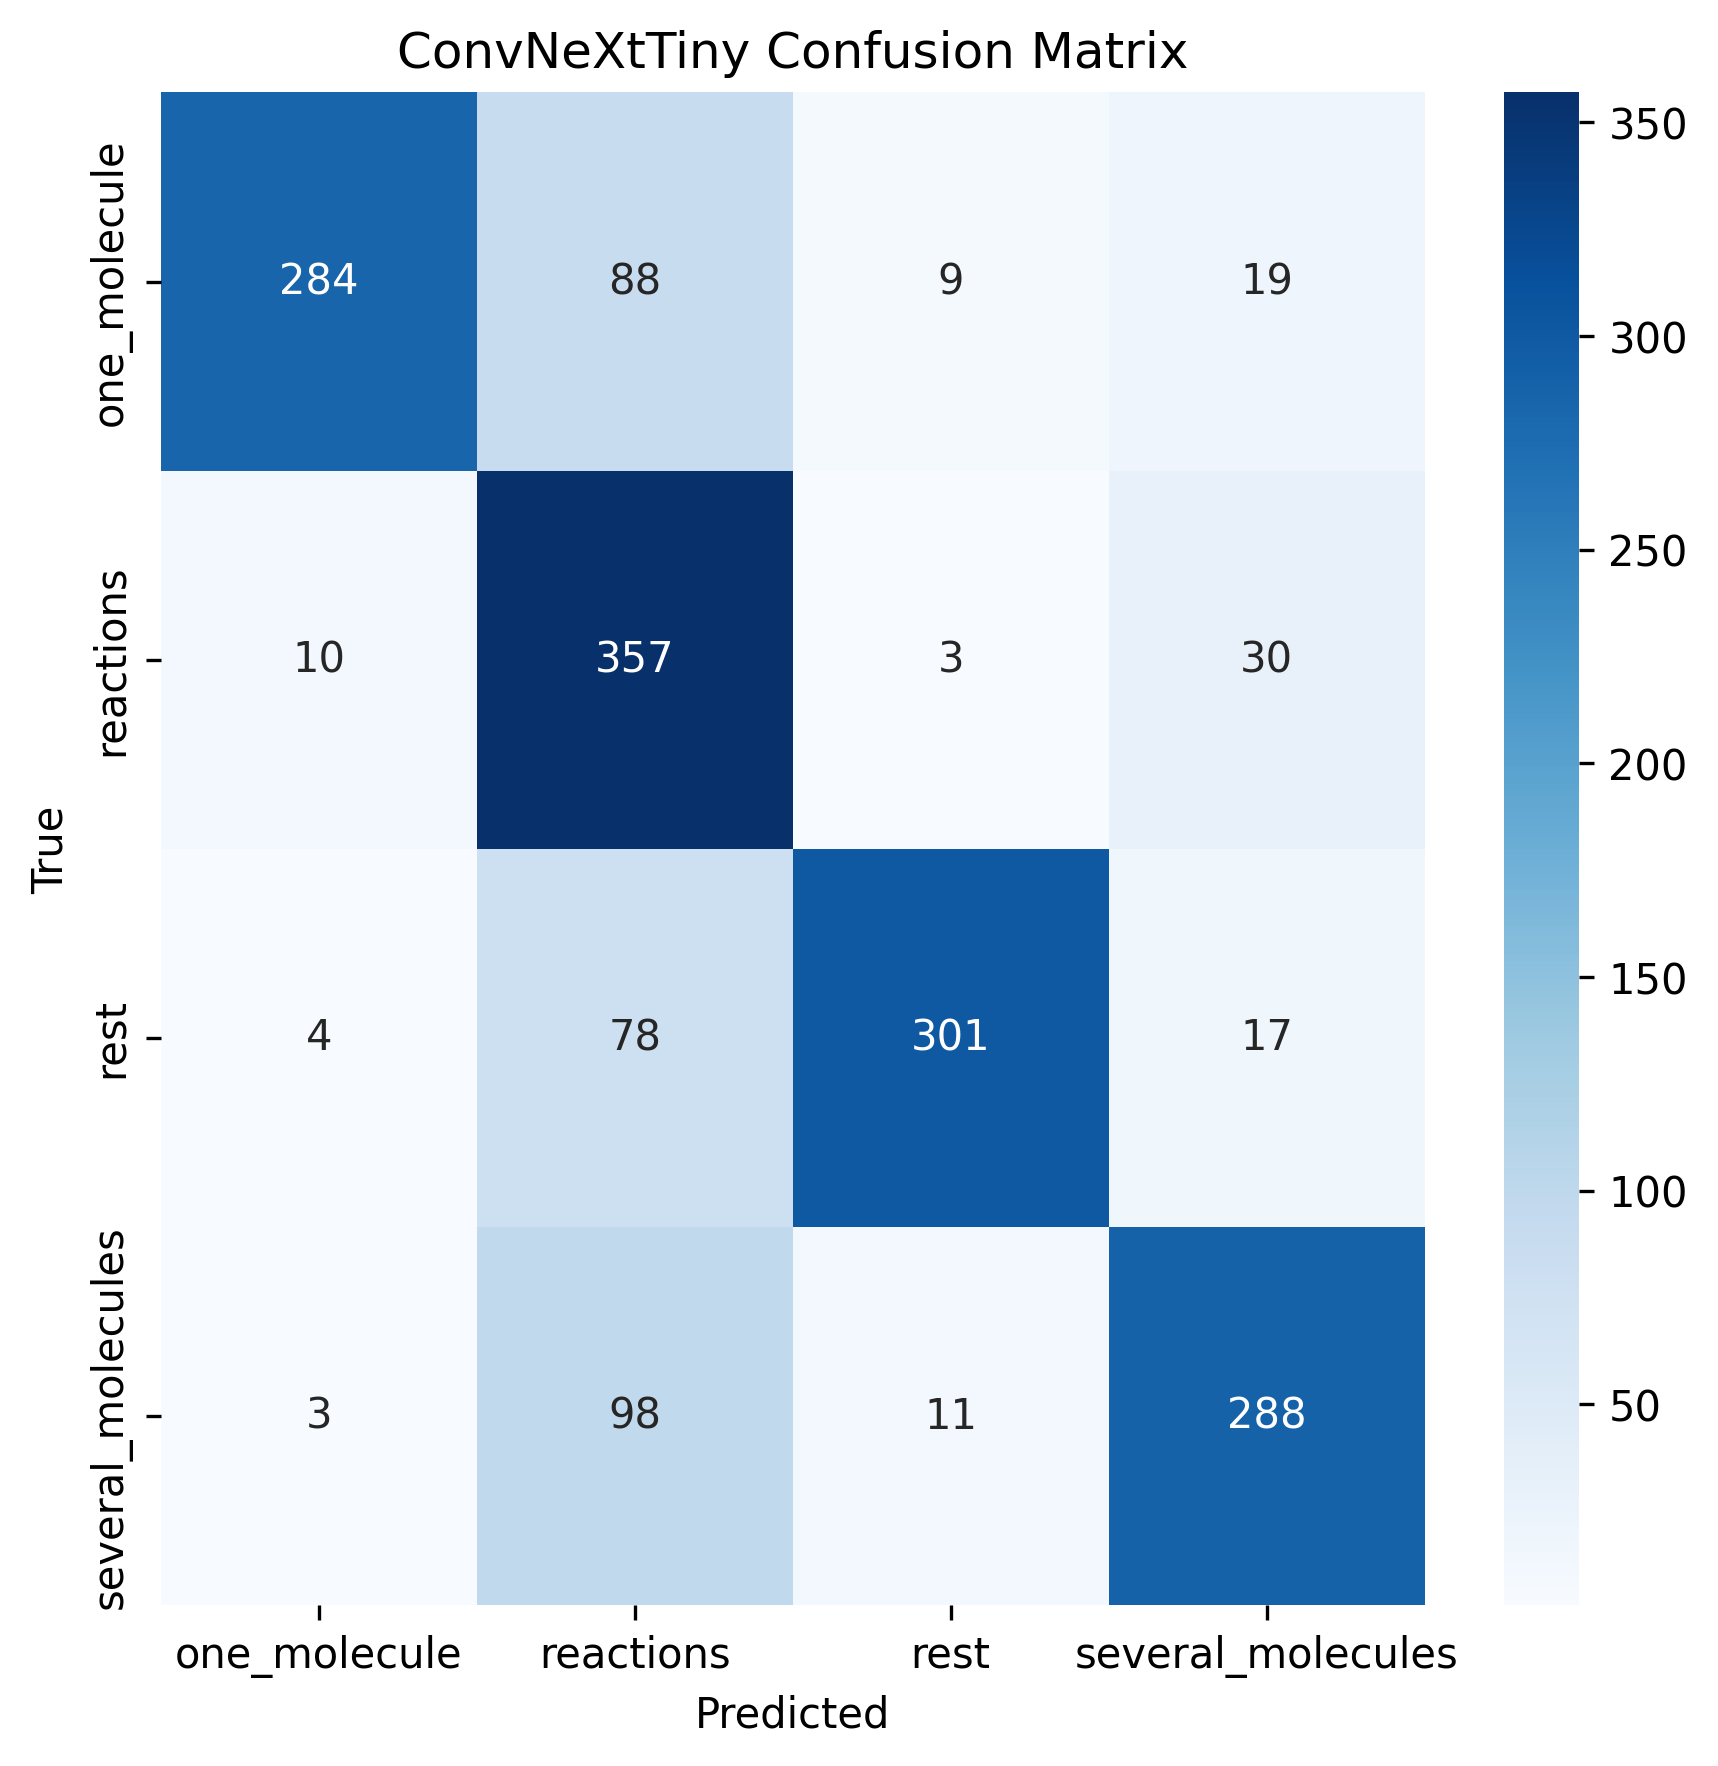
\includegraphics[width=\textwidth]{chemical_classification_models/Confusion_Matrix/ConvNeXtTiny_Confusion_Matrix.png}
  \caption{ConvNeXtTiny}
  \label{fig:cm_convnext}
\end{subfigure}
\caption{Confusion Heatmaps --- MobileNetV2, Xception, EfficientNetB4, ConvNeXtTiny}
\label{fig:confusion_matrices_g2}
\end{figure}

\begin{figure}[H]
\centering
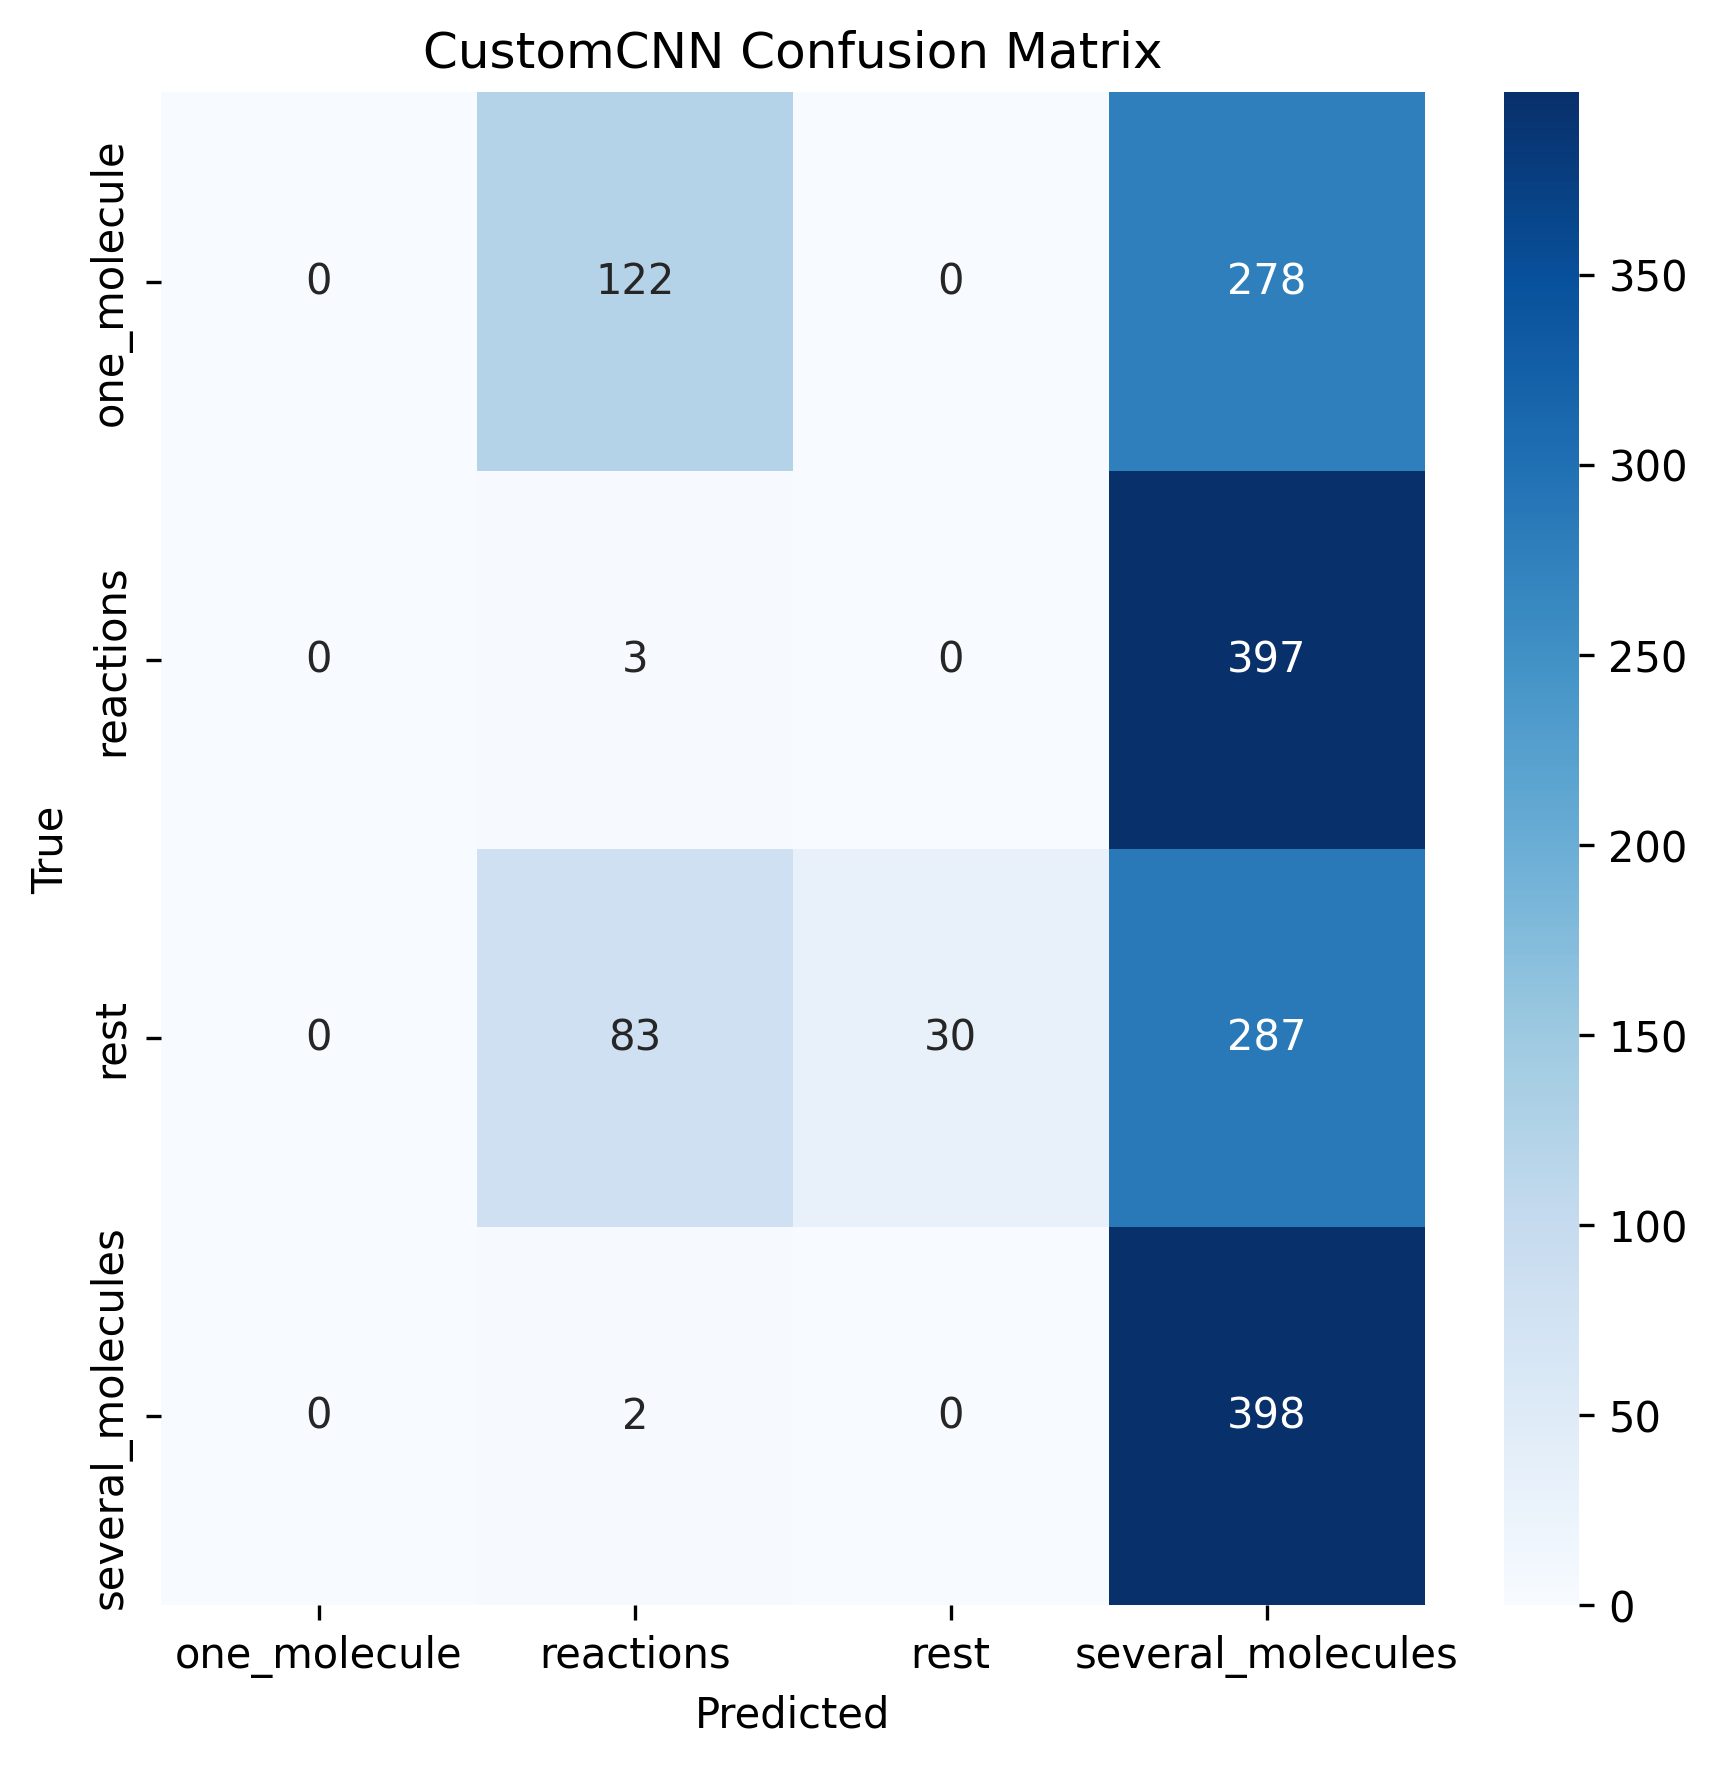
\includegraphics[width=0.66\textwidth]{chemical_classification_models/Confusion_Matrix/CustomCNN_Confusion_Matrix.png}
\caption{Confusion Heatmap --- Custom CNN}
\label{fig:cm_custom}
\end{figure}

% ==============================================================
%  SECTION 12: ROC CURVES
% ==============================================================
\section{ROC Curve \& AUC}

Multi-class ROC curves were computed using the \textbf{One-vs-Rest (OvR)} strategy with label binarization. The AUC (Area Under the Curve) was macro-averaged across all 4 classes. A higher AUC indicates better ability to distinguish between classes.

\begin{table}[H]
\centering
\caption{ROC Area Under the Curve (AUC) Summary}
\label{tab:auc_metrics}
\rowcolors{2}{LightGray}{white}
\begin{tabular}{l c}
  \toprule
  \textbf{Model} & \textbf{AUC (Macro-Avg)} \\
  \midrule
  \rowcolor{green!12} \textbf{VGG16} & \textbf{0.9890} \\
  InceptionV3    & 0.9846 \\
  DenseNet121    & 0.9832 \\
  ResNet50V2     & 0.9821 \\
  MobileNetV2    & 0.9614 \\
  Xception       & 0.9554 \\
  ConvNeXtTiny   & 0.9459 \\
  EfficientNetB4 & 0.7105 \\
  CustomCNN      & 0.6743 \\
  \bottomrule
\end{tabular}
\end{table}

\subsection{ROC Curves Grid}

\begin{figure}[H]
\centering
\begin{subfigure}{0.48\textwidth}
  \centering
  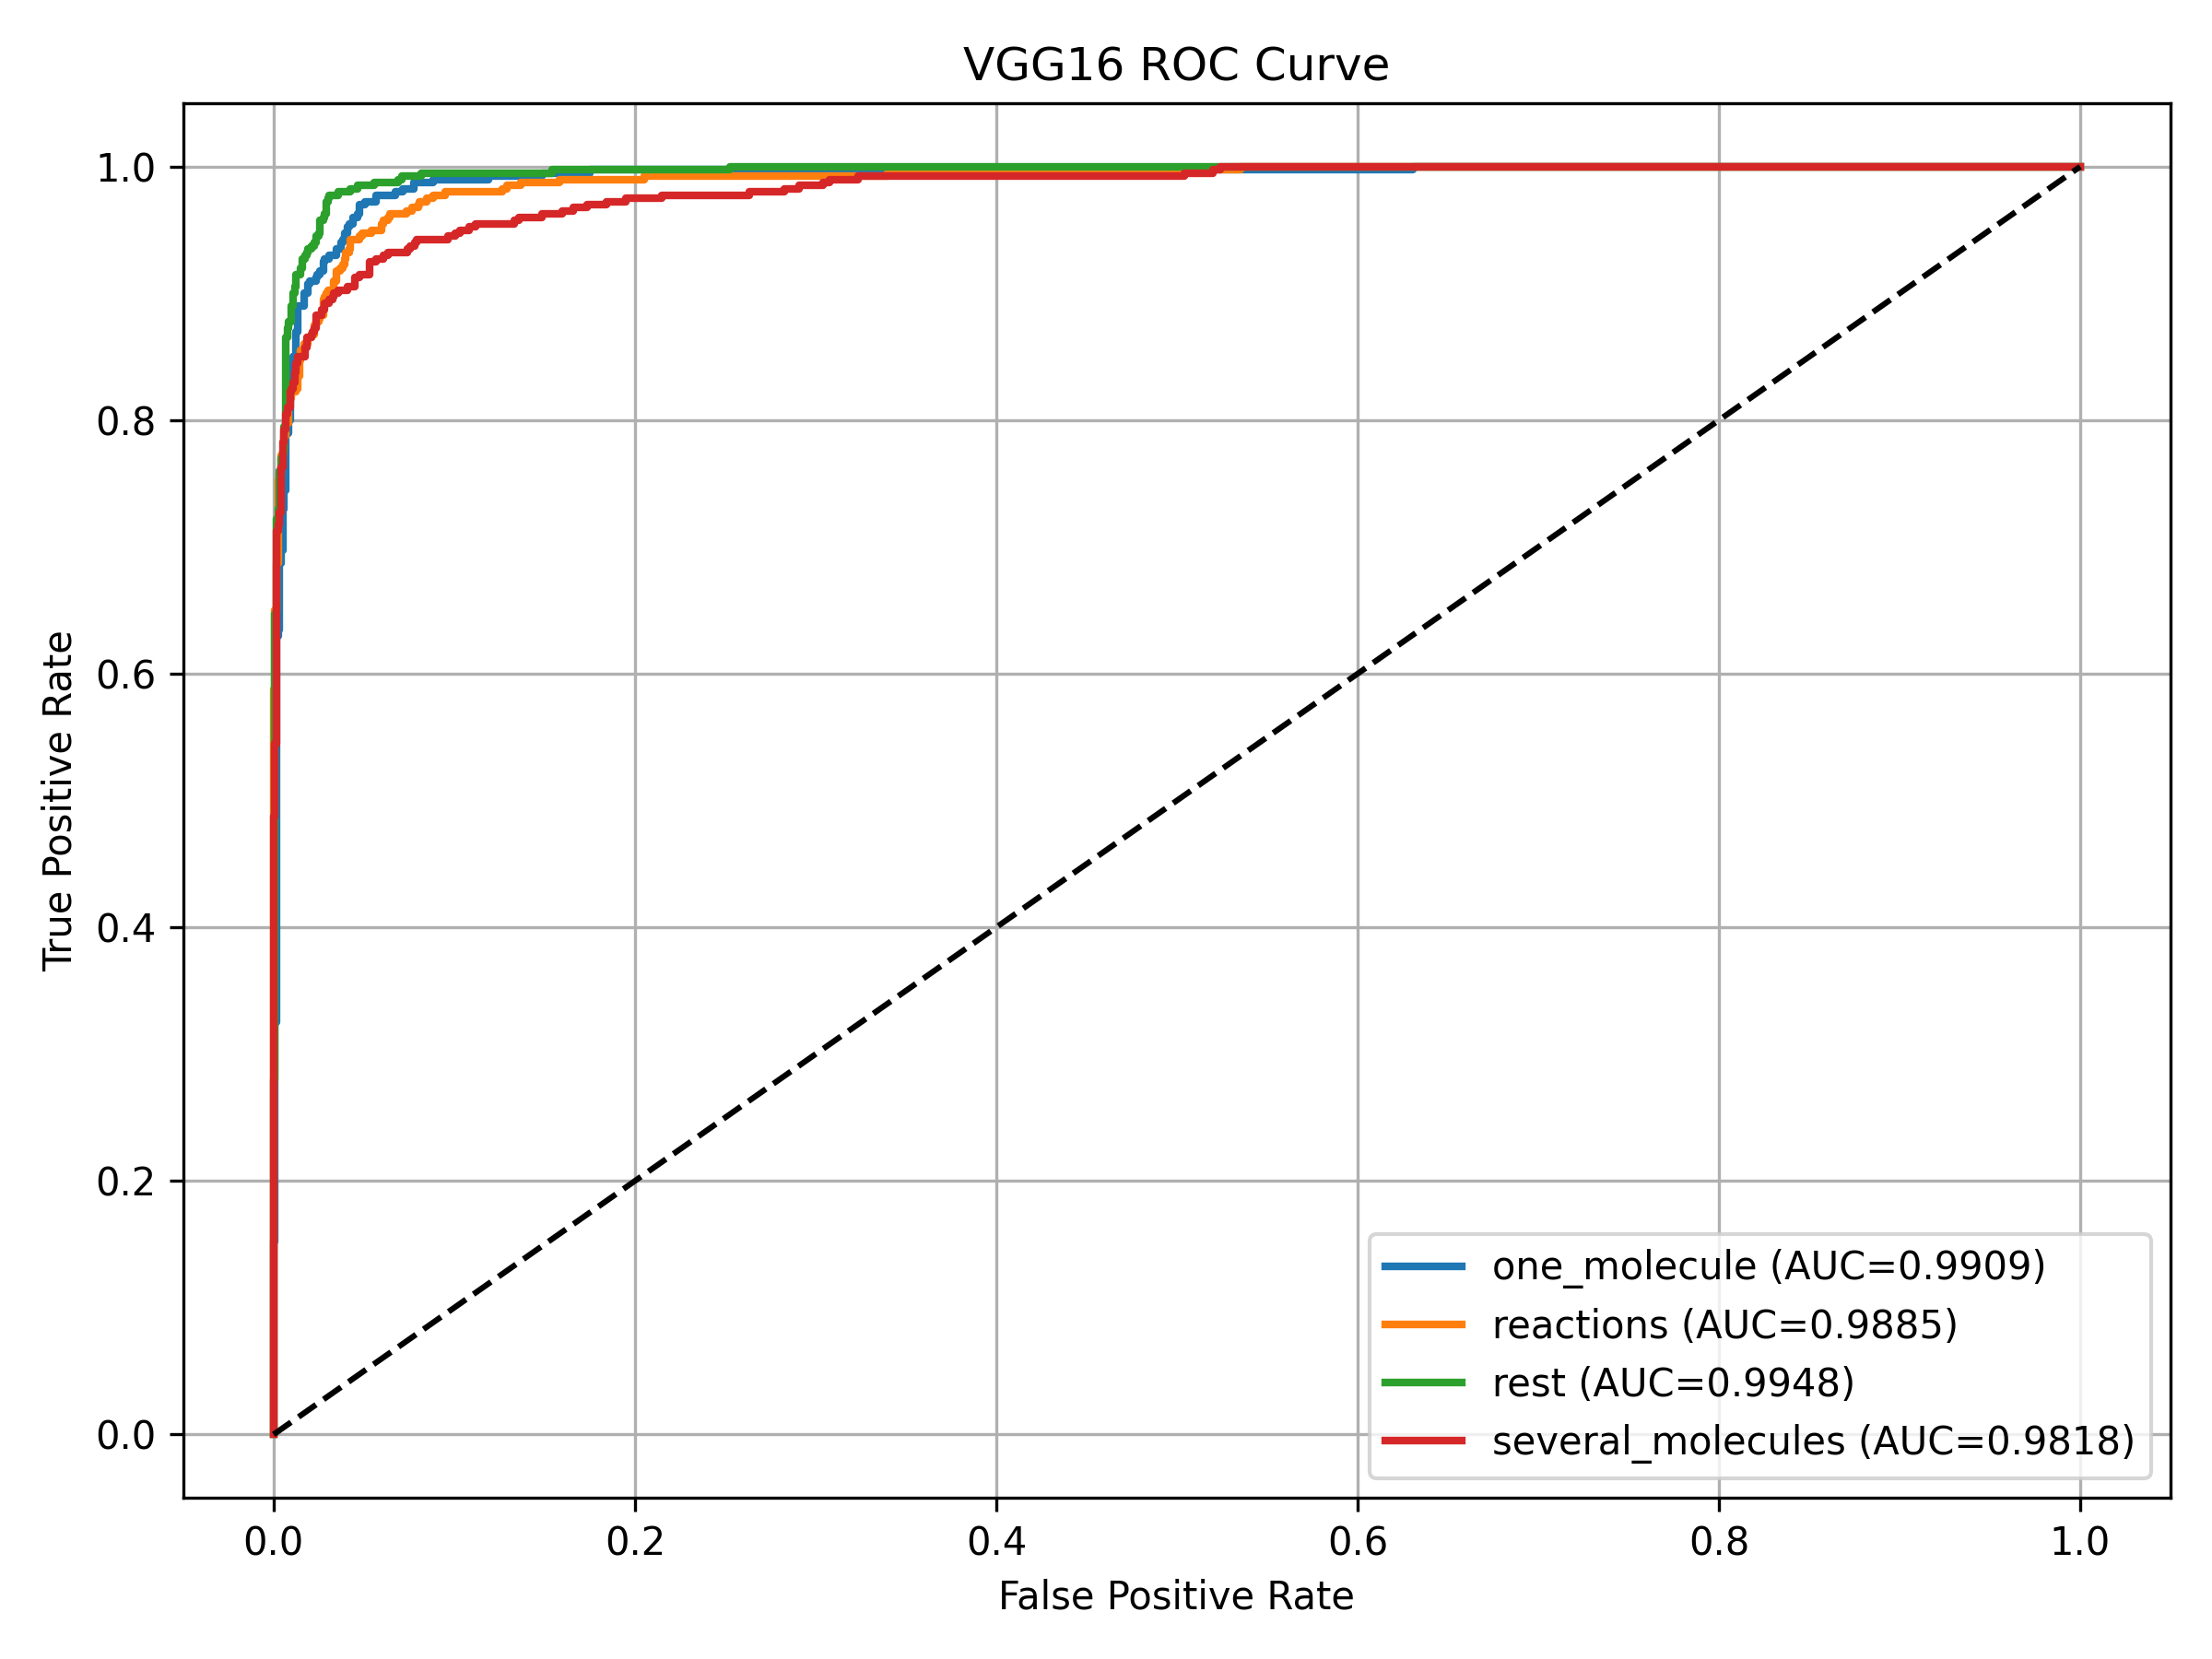
\includegraphics[width=\textwidth]{chemical_classification_models/Results/ROC_Curves/VGG16_ROC.png}
  \caption{VGG16}
  \label{fig:roc_vgg}
\end{subfigure}
\hfill
\begin{subfigure}{0.48\textwidth}
  \centering
  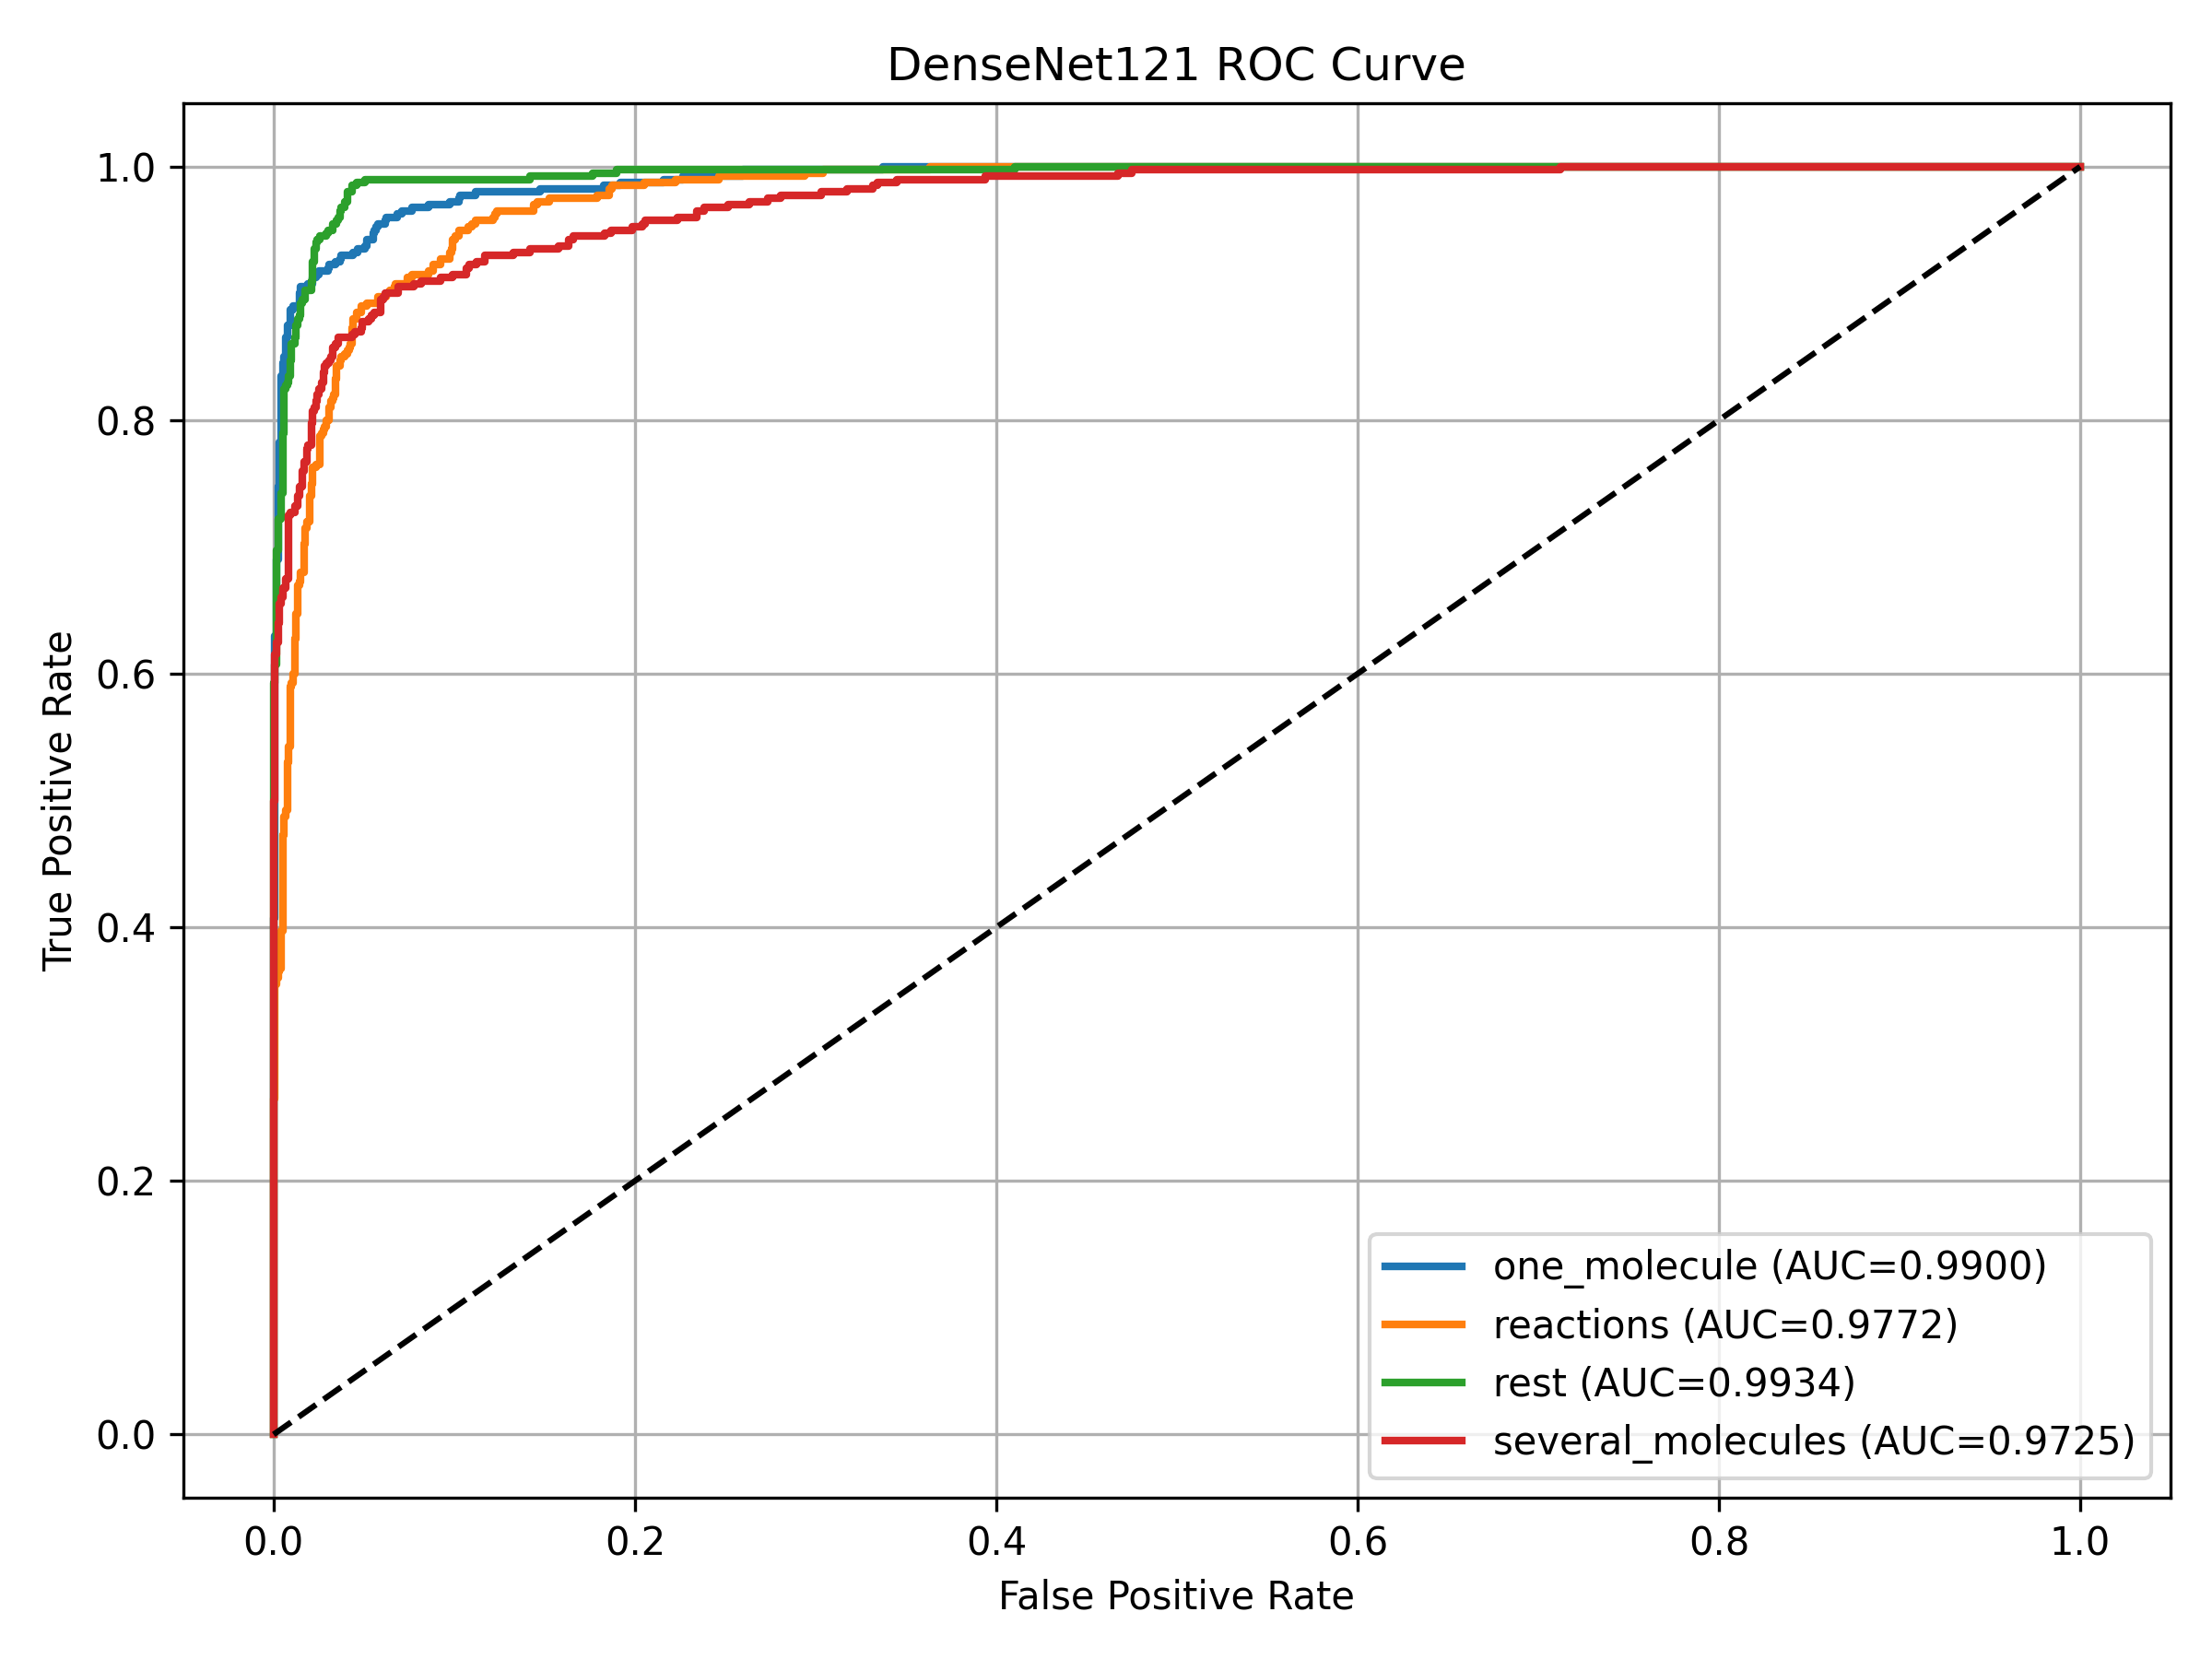
\includegraphics[width=\textwidth]{chemical_classification_models/Results/ROC_Curves/DenseNet121_ROC.png}
  \caption{DenseNet121}
  \label{fig:roc_dense}
\end{subfigure}

\vspace{0.4cm}

\begin{subfigure}{0.48\textwidth}
  \centering
  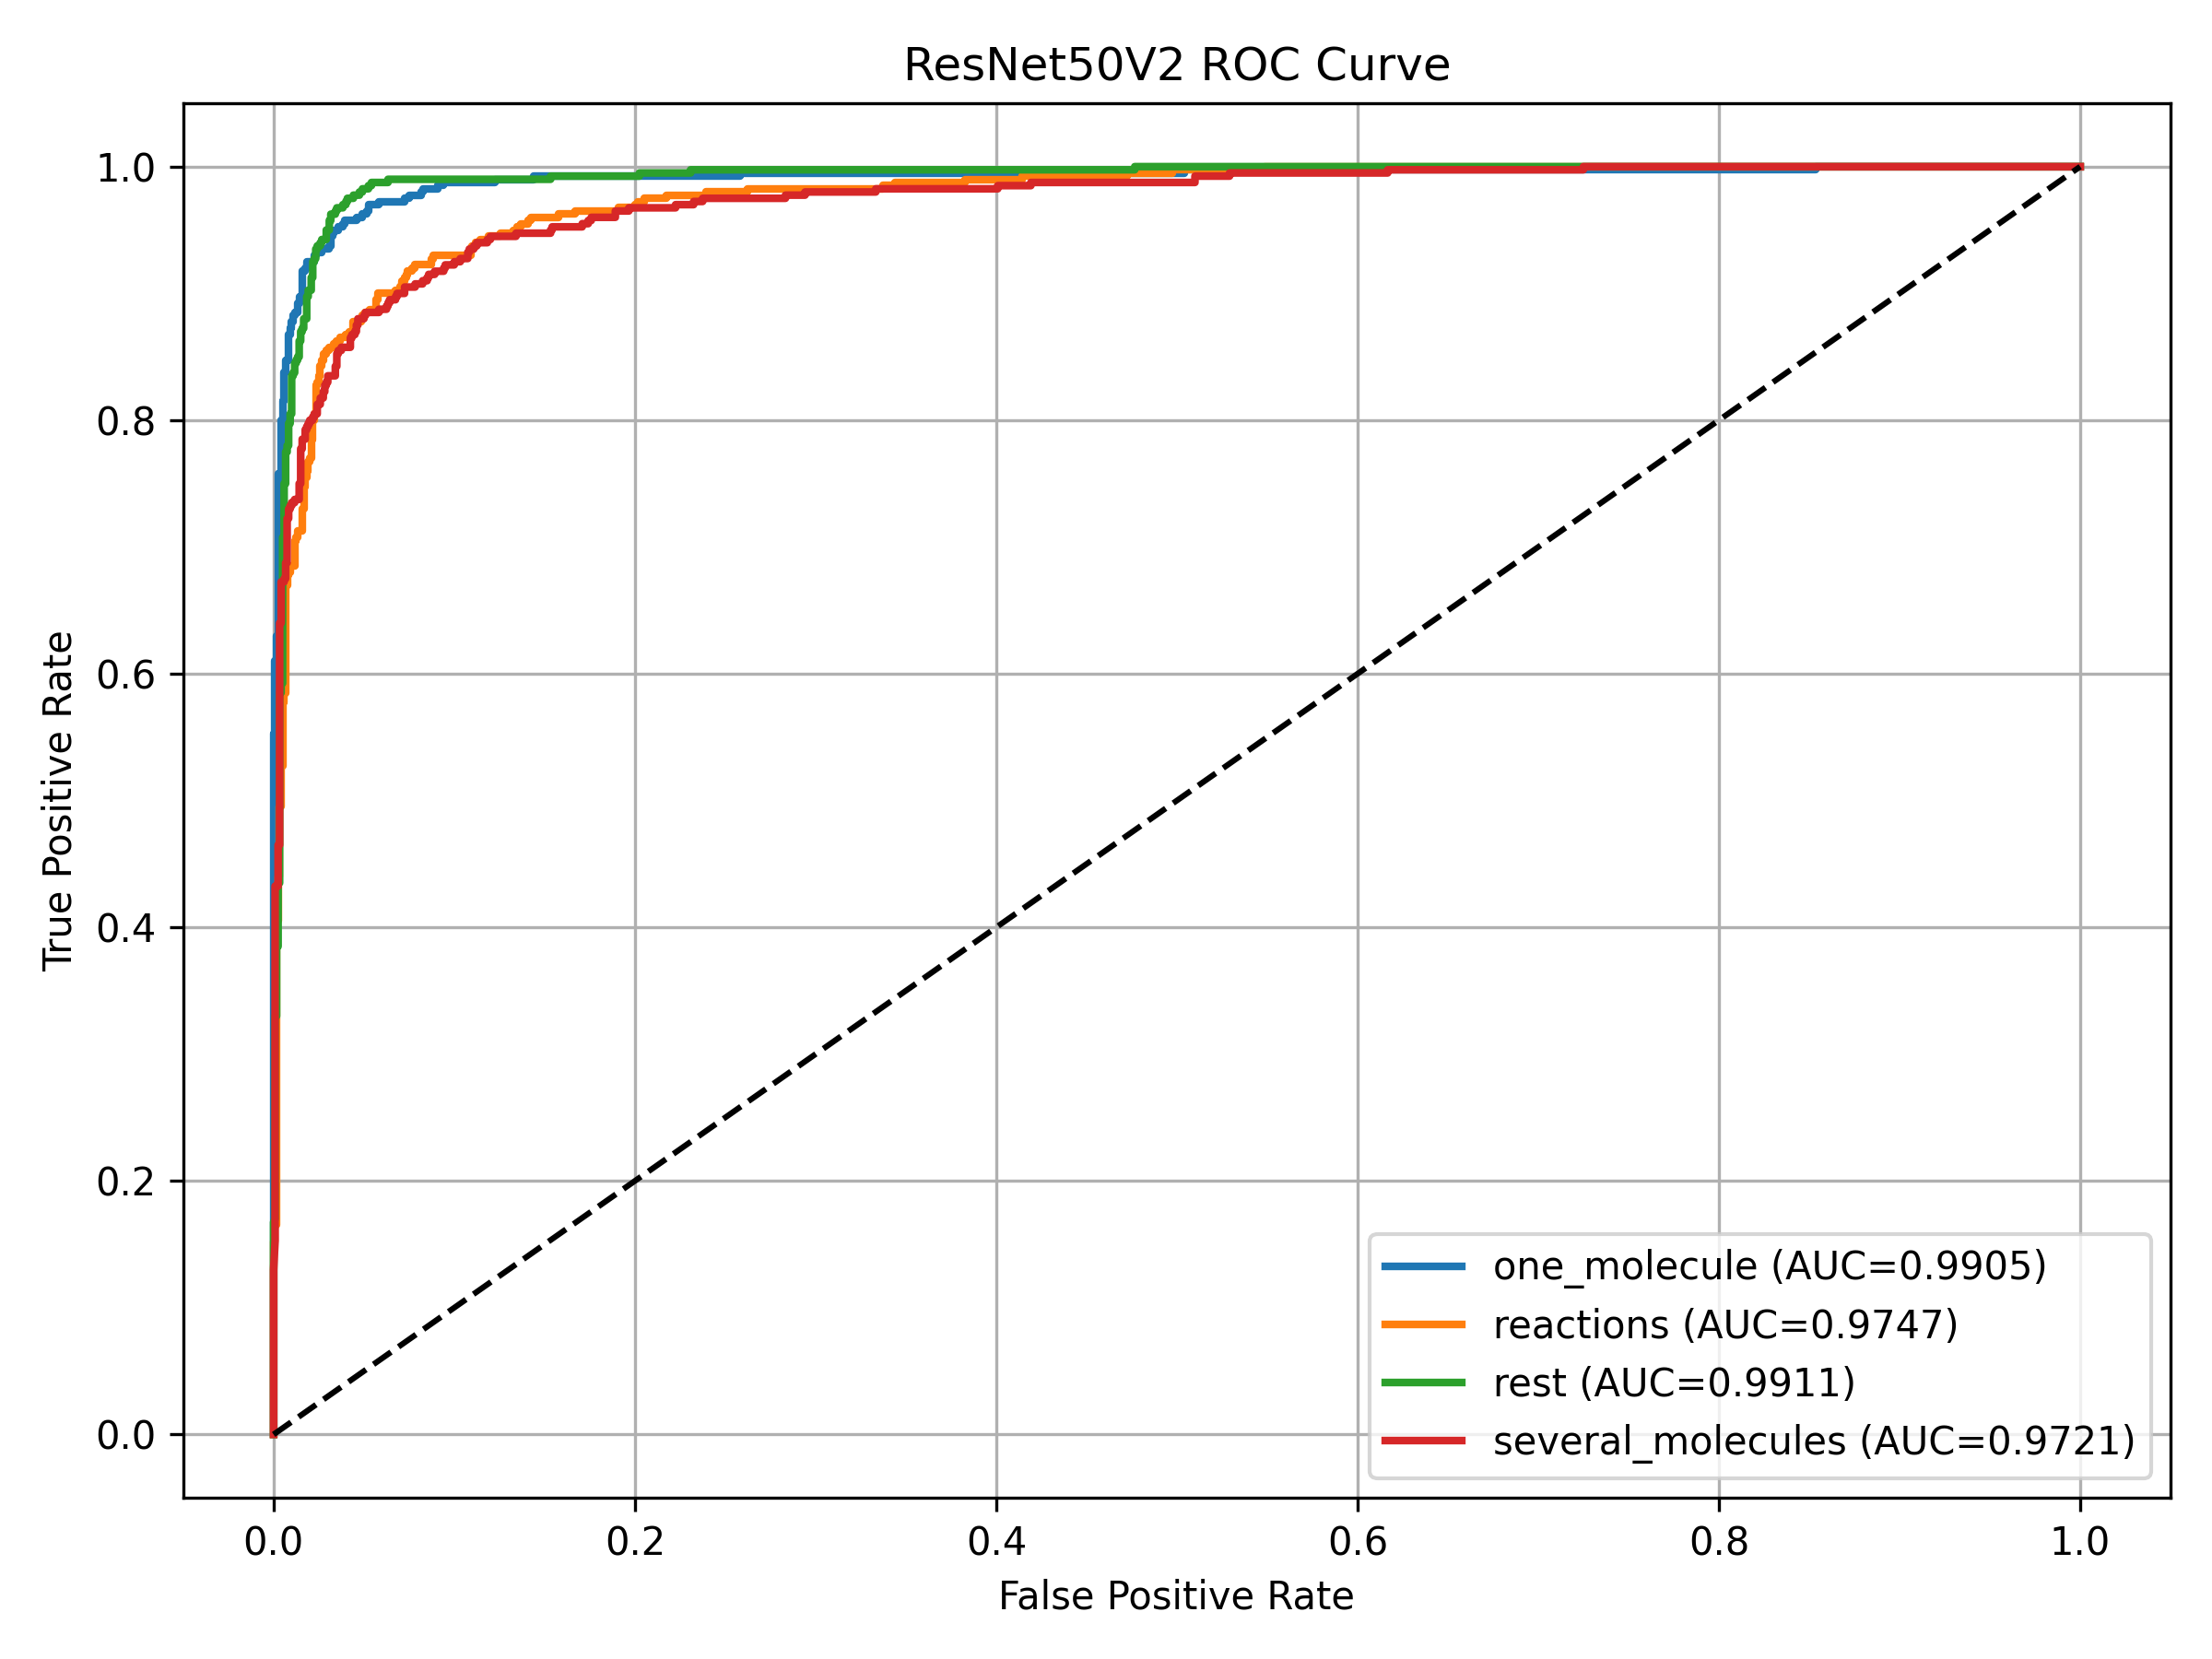
\includegraphics[width=\textwidth]{chemical_classification_models/Results//ROC_Curves/ResNet50V2_ROC.png}
  \caption{ResNet50V2}
  \label{fig:roc_resnet}
\end{subfigure}
\hfill
\begin{subfigure}{0.48\textwidth}
  \centering
  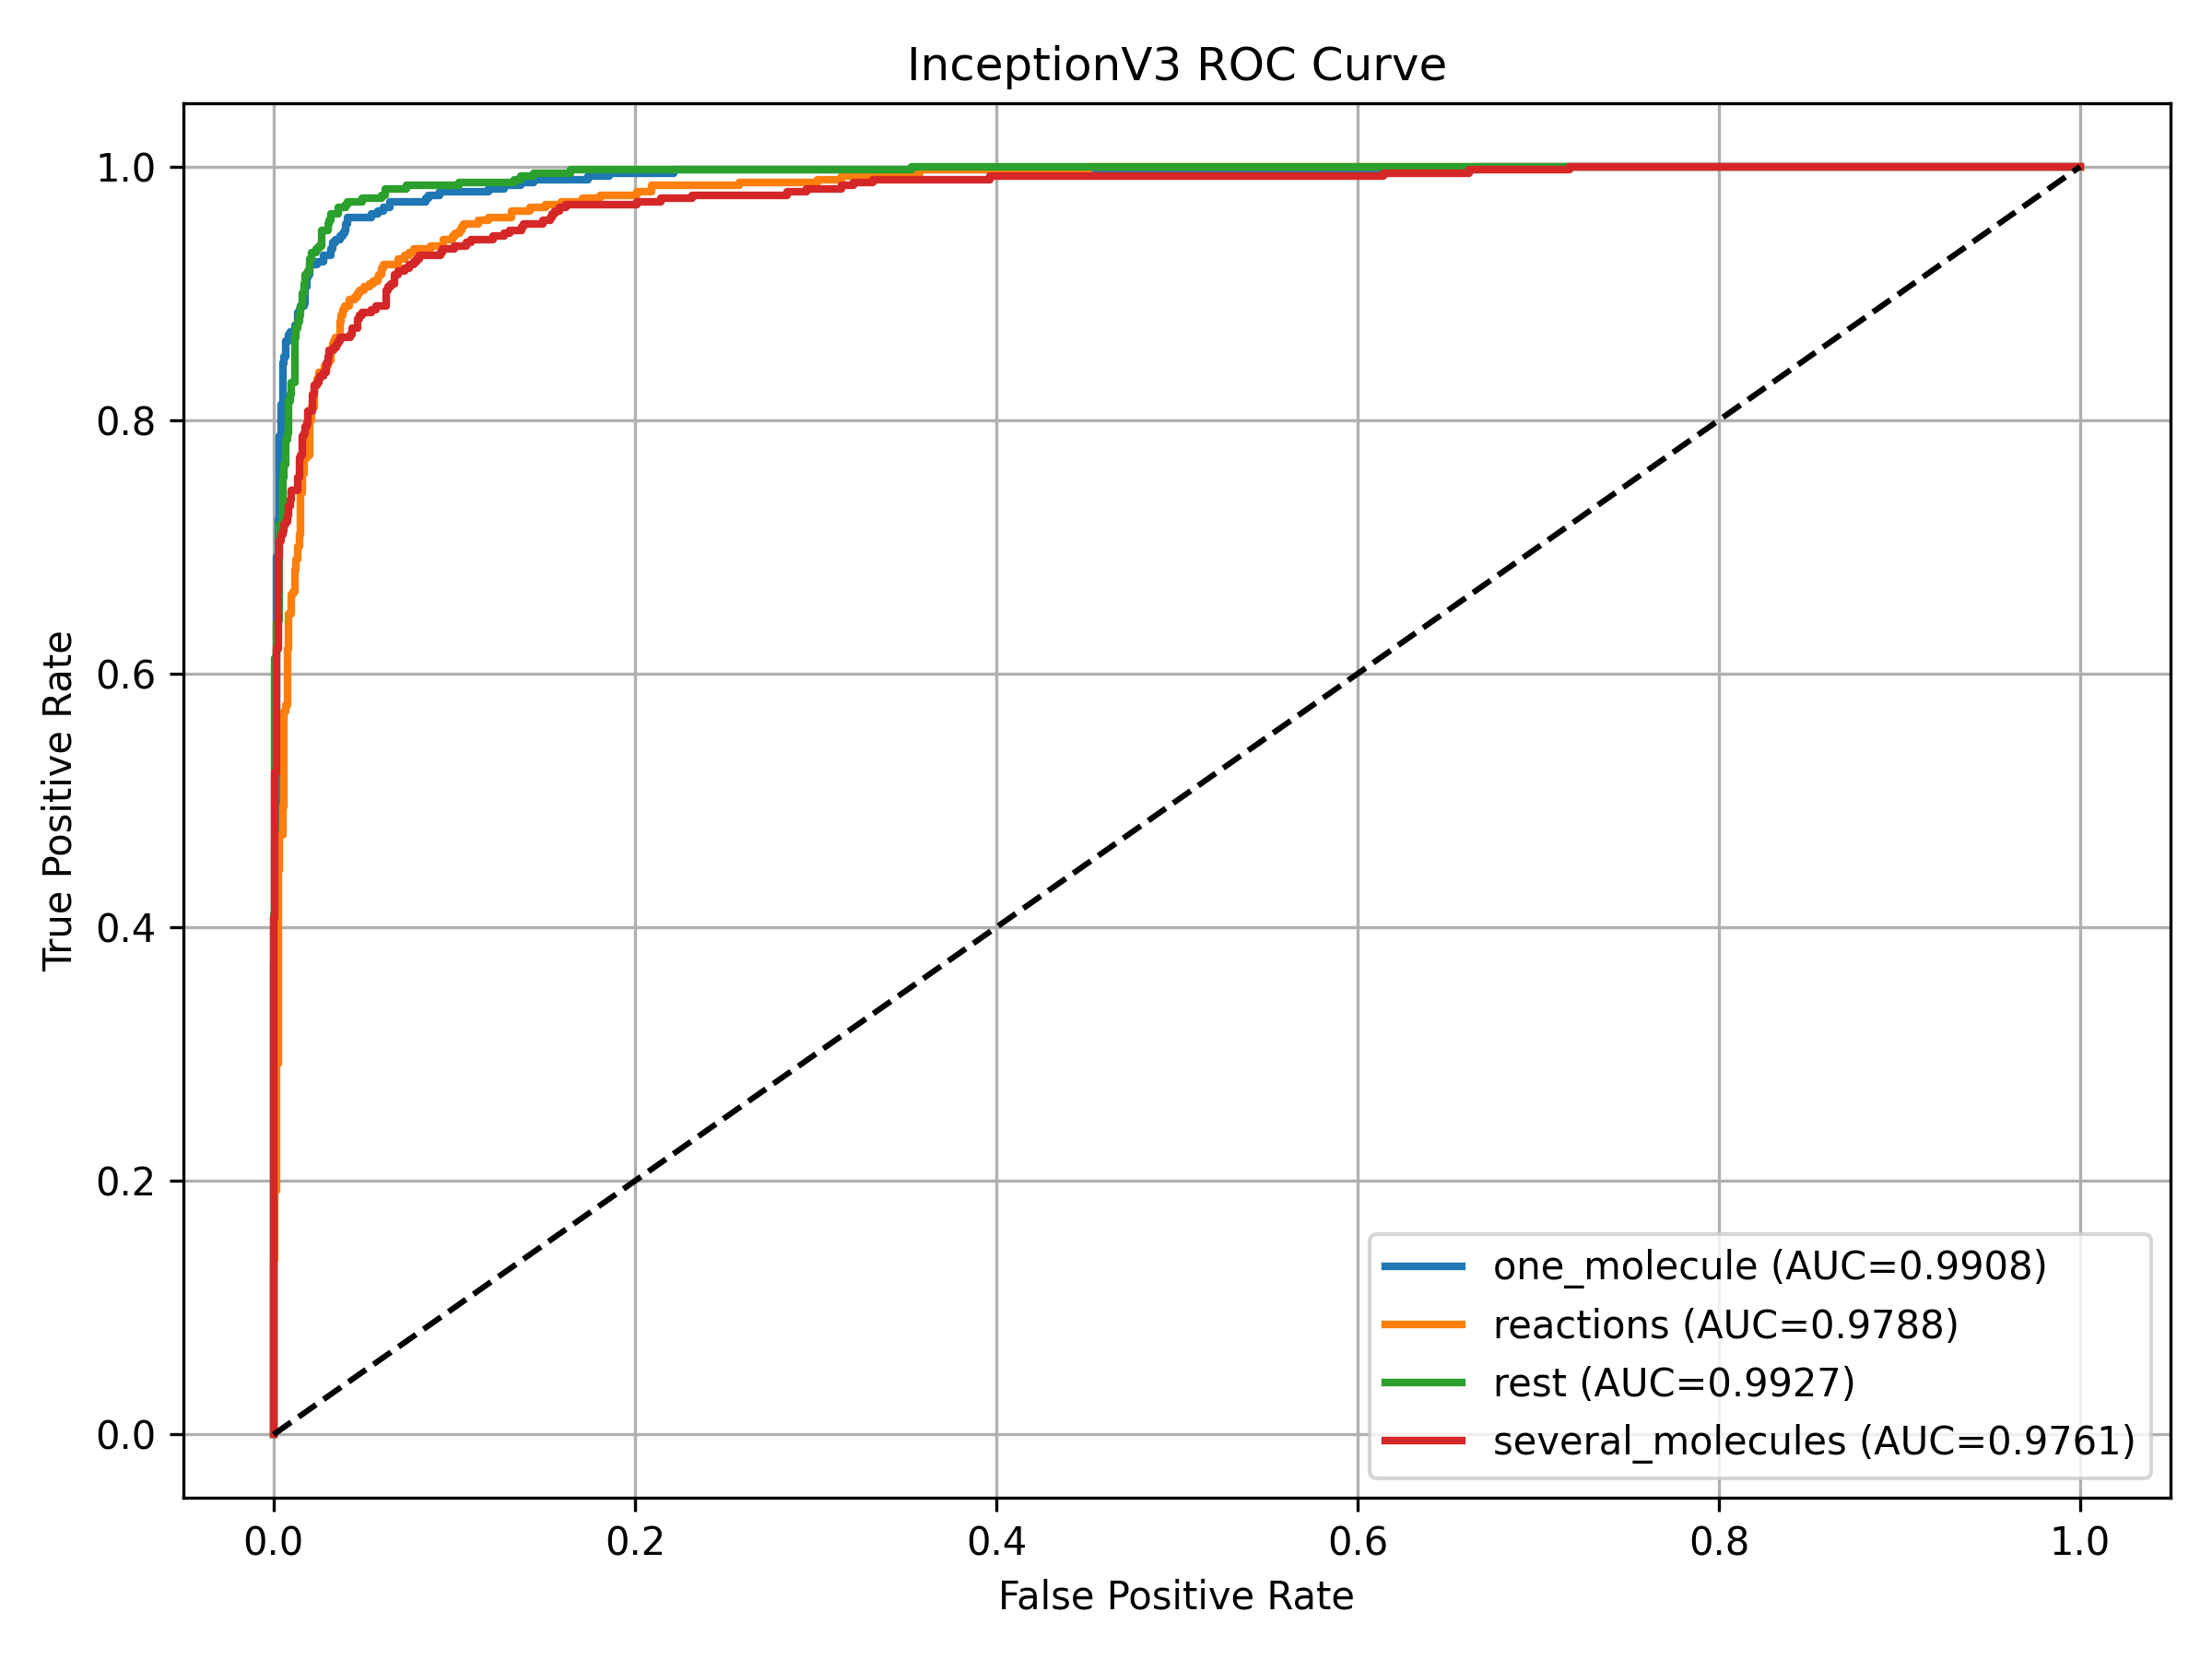
\includegraphics[width=\textwidth]{chemical_classification_models/Results/ROC_Curves/InceptionV3_ROC.png}
  \caption{InceptionV3}
  \label{fig:roc_inception}
\end{subfigure}
\caption{One-vs-Rest (OvR) ROC Curves --- VGG16, DenseNet121, ResNet50V2, InceptionV3}
\label{fig:roc_curves_g1}
\end{figure}

\begin{figure}[H]
\centering
\begin{subfigure}{0.48\textwidth}
  \centering
  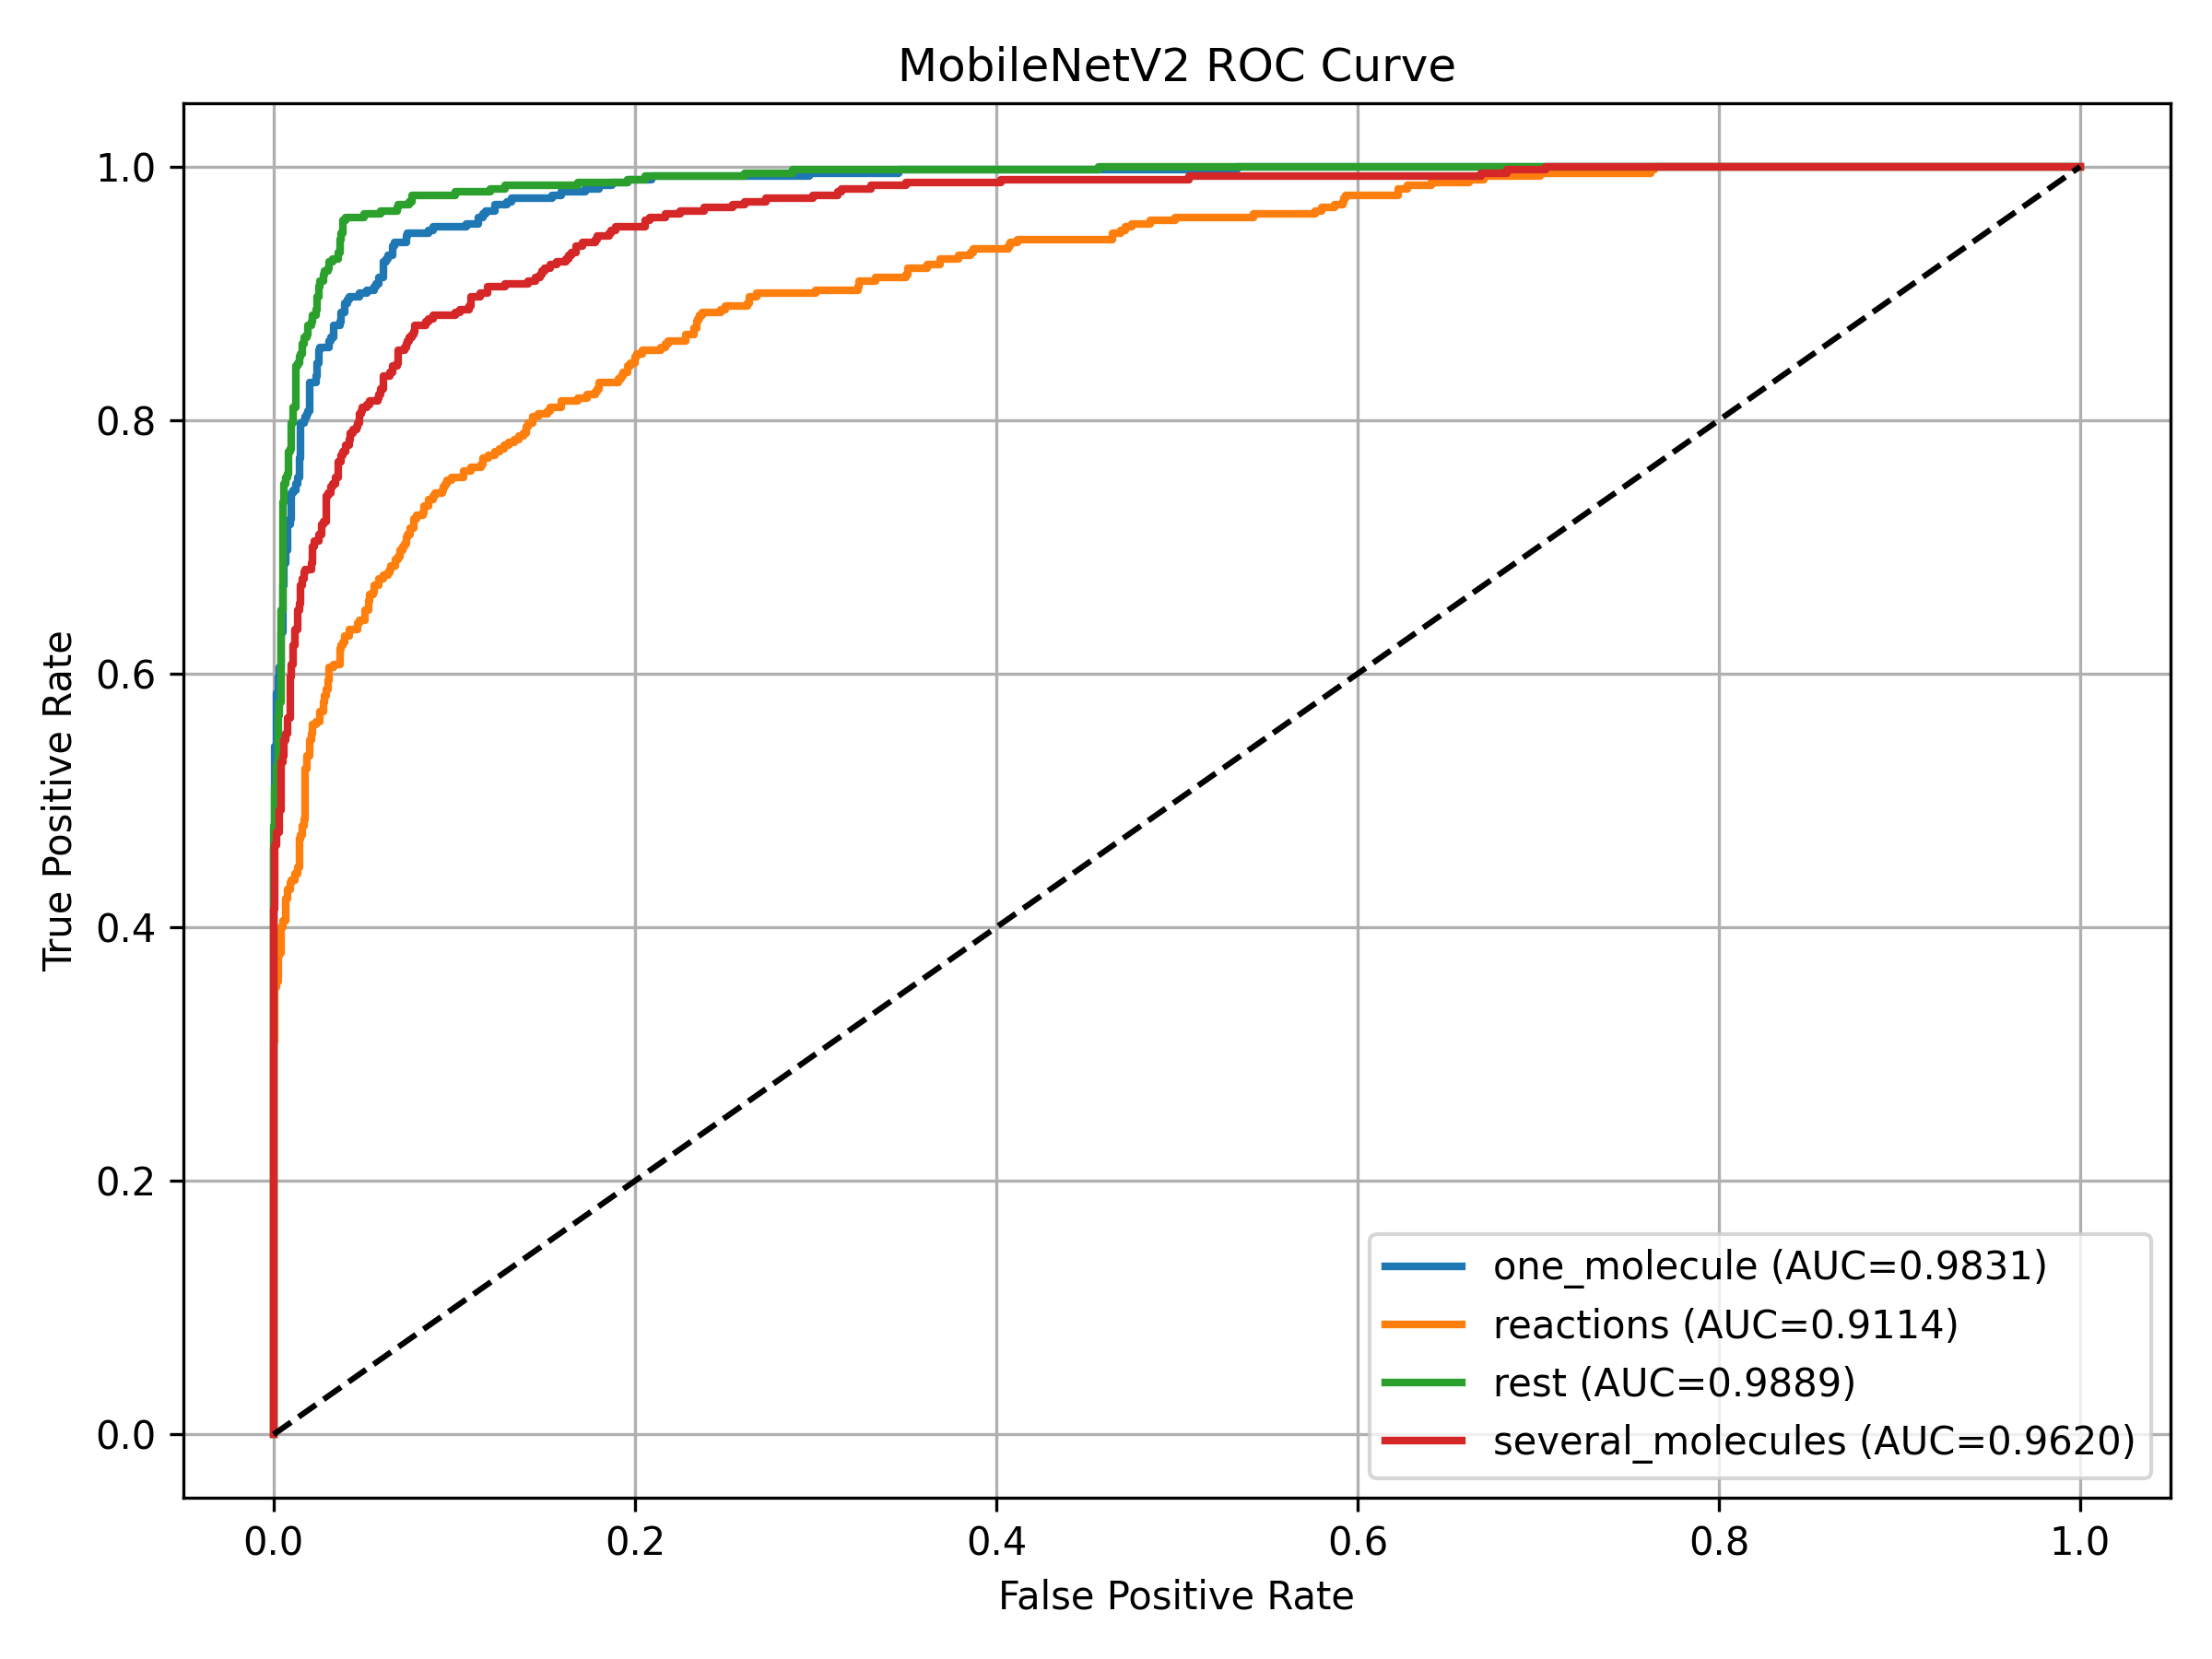
\includegraphics[width=\textwidth]{chemical_classification_models/Results/ROC_Curves/MobileNetV2_ROC.png}
  \caption{MobileNetV2}
  \label{fig:roc_mobile}
\end{subfigure}
\hfill
\begin{subfigure}{0.48\textwidth}
  \centering
  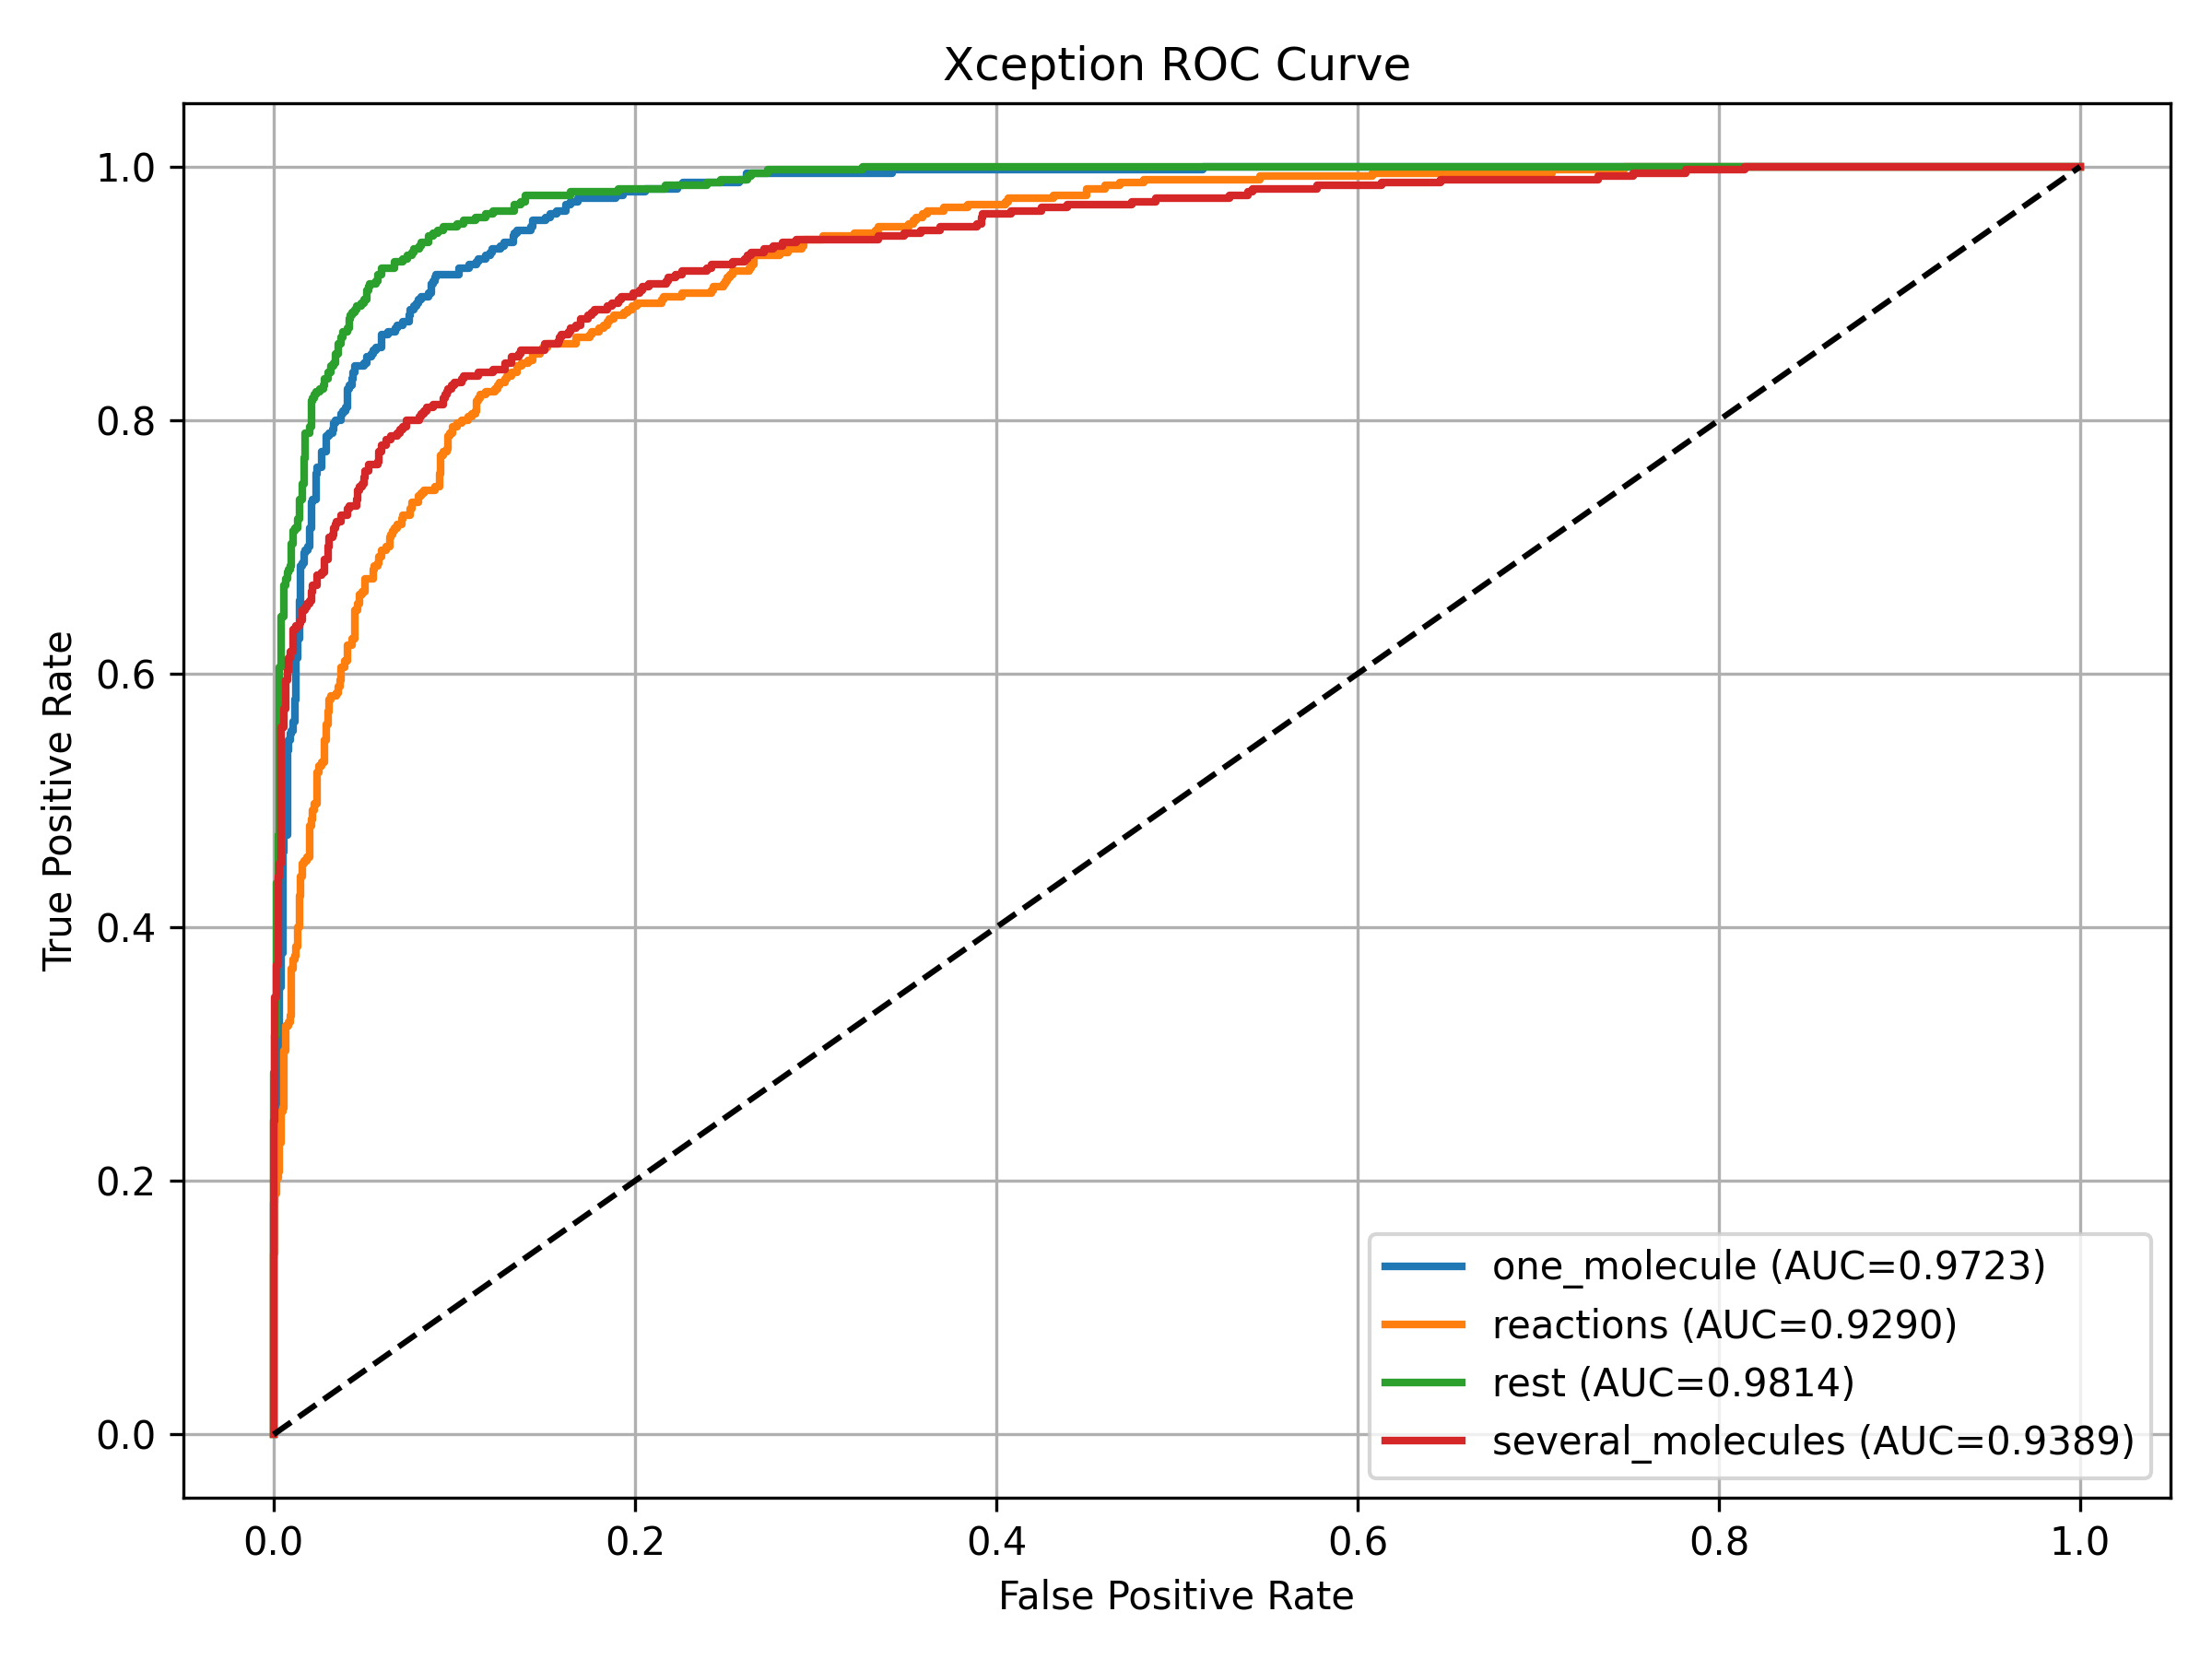
\includegraphics[width=\textwidth]{chemical_classification_models/Results/ROC_Curves/Xception_ROC.png}
  \caption{Xception}
  \label{fig:roc_xception}
\end{subfigure}

\vspace{0.4cm}

\begin{subfigure}{0.48\textwidth}
  \centering
  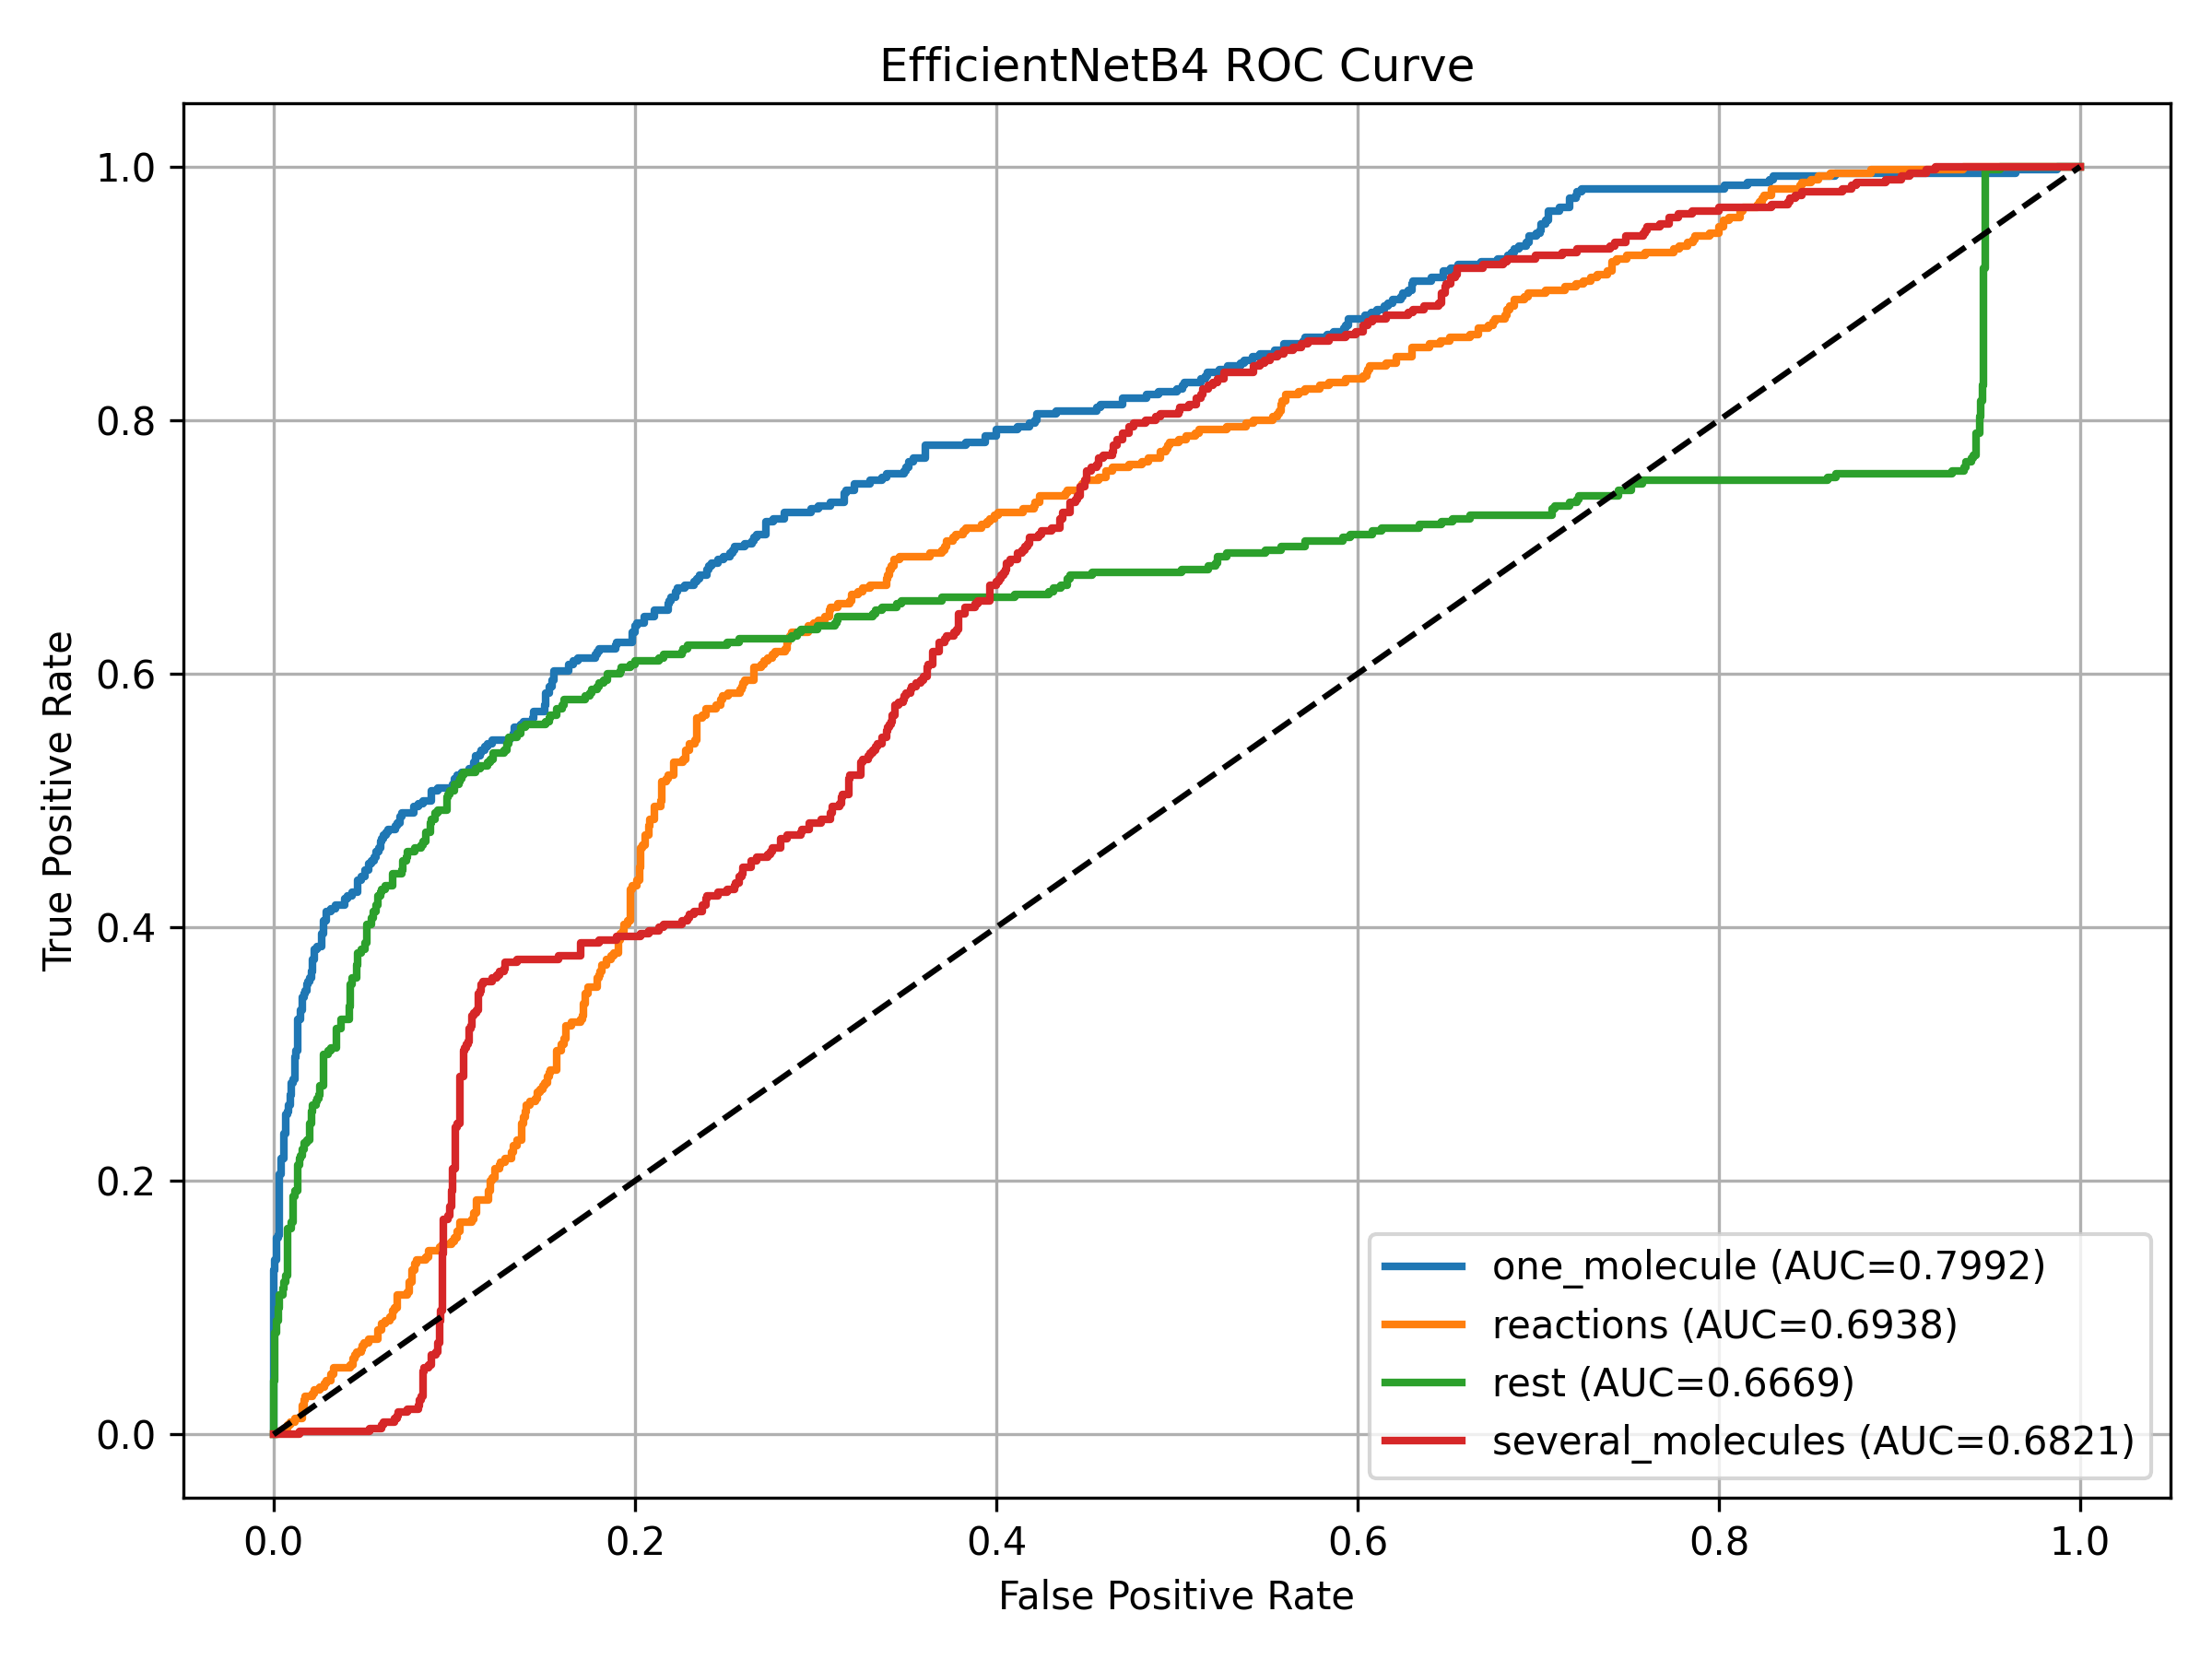
\includegraphics[width=\textwidth]{chemical_classification_models/Results/ROC_Curves/EfficientNetB4_ROC.png}
  \caption{EfficientNetB4}
  \label{fig:roc_effnet}
\end{subfigure}
\hfill
\begin{subfigure}{0.48\textwidth}
  \centering
  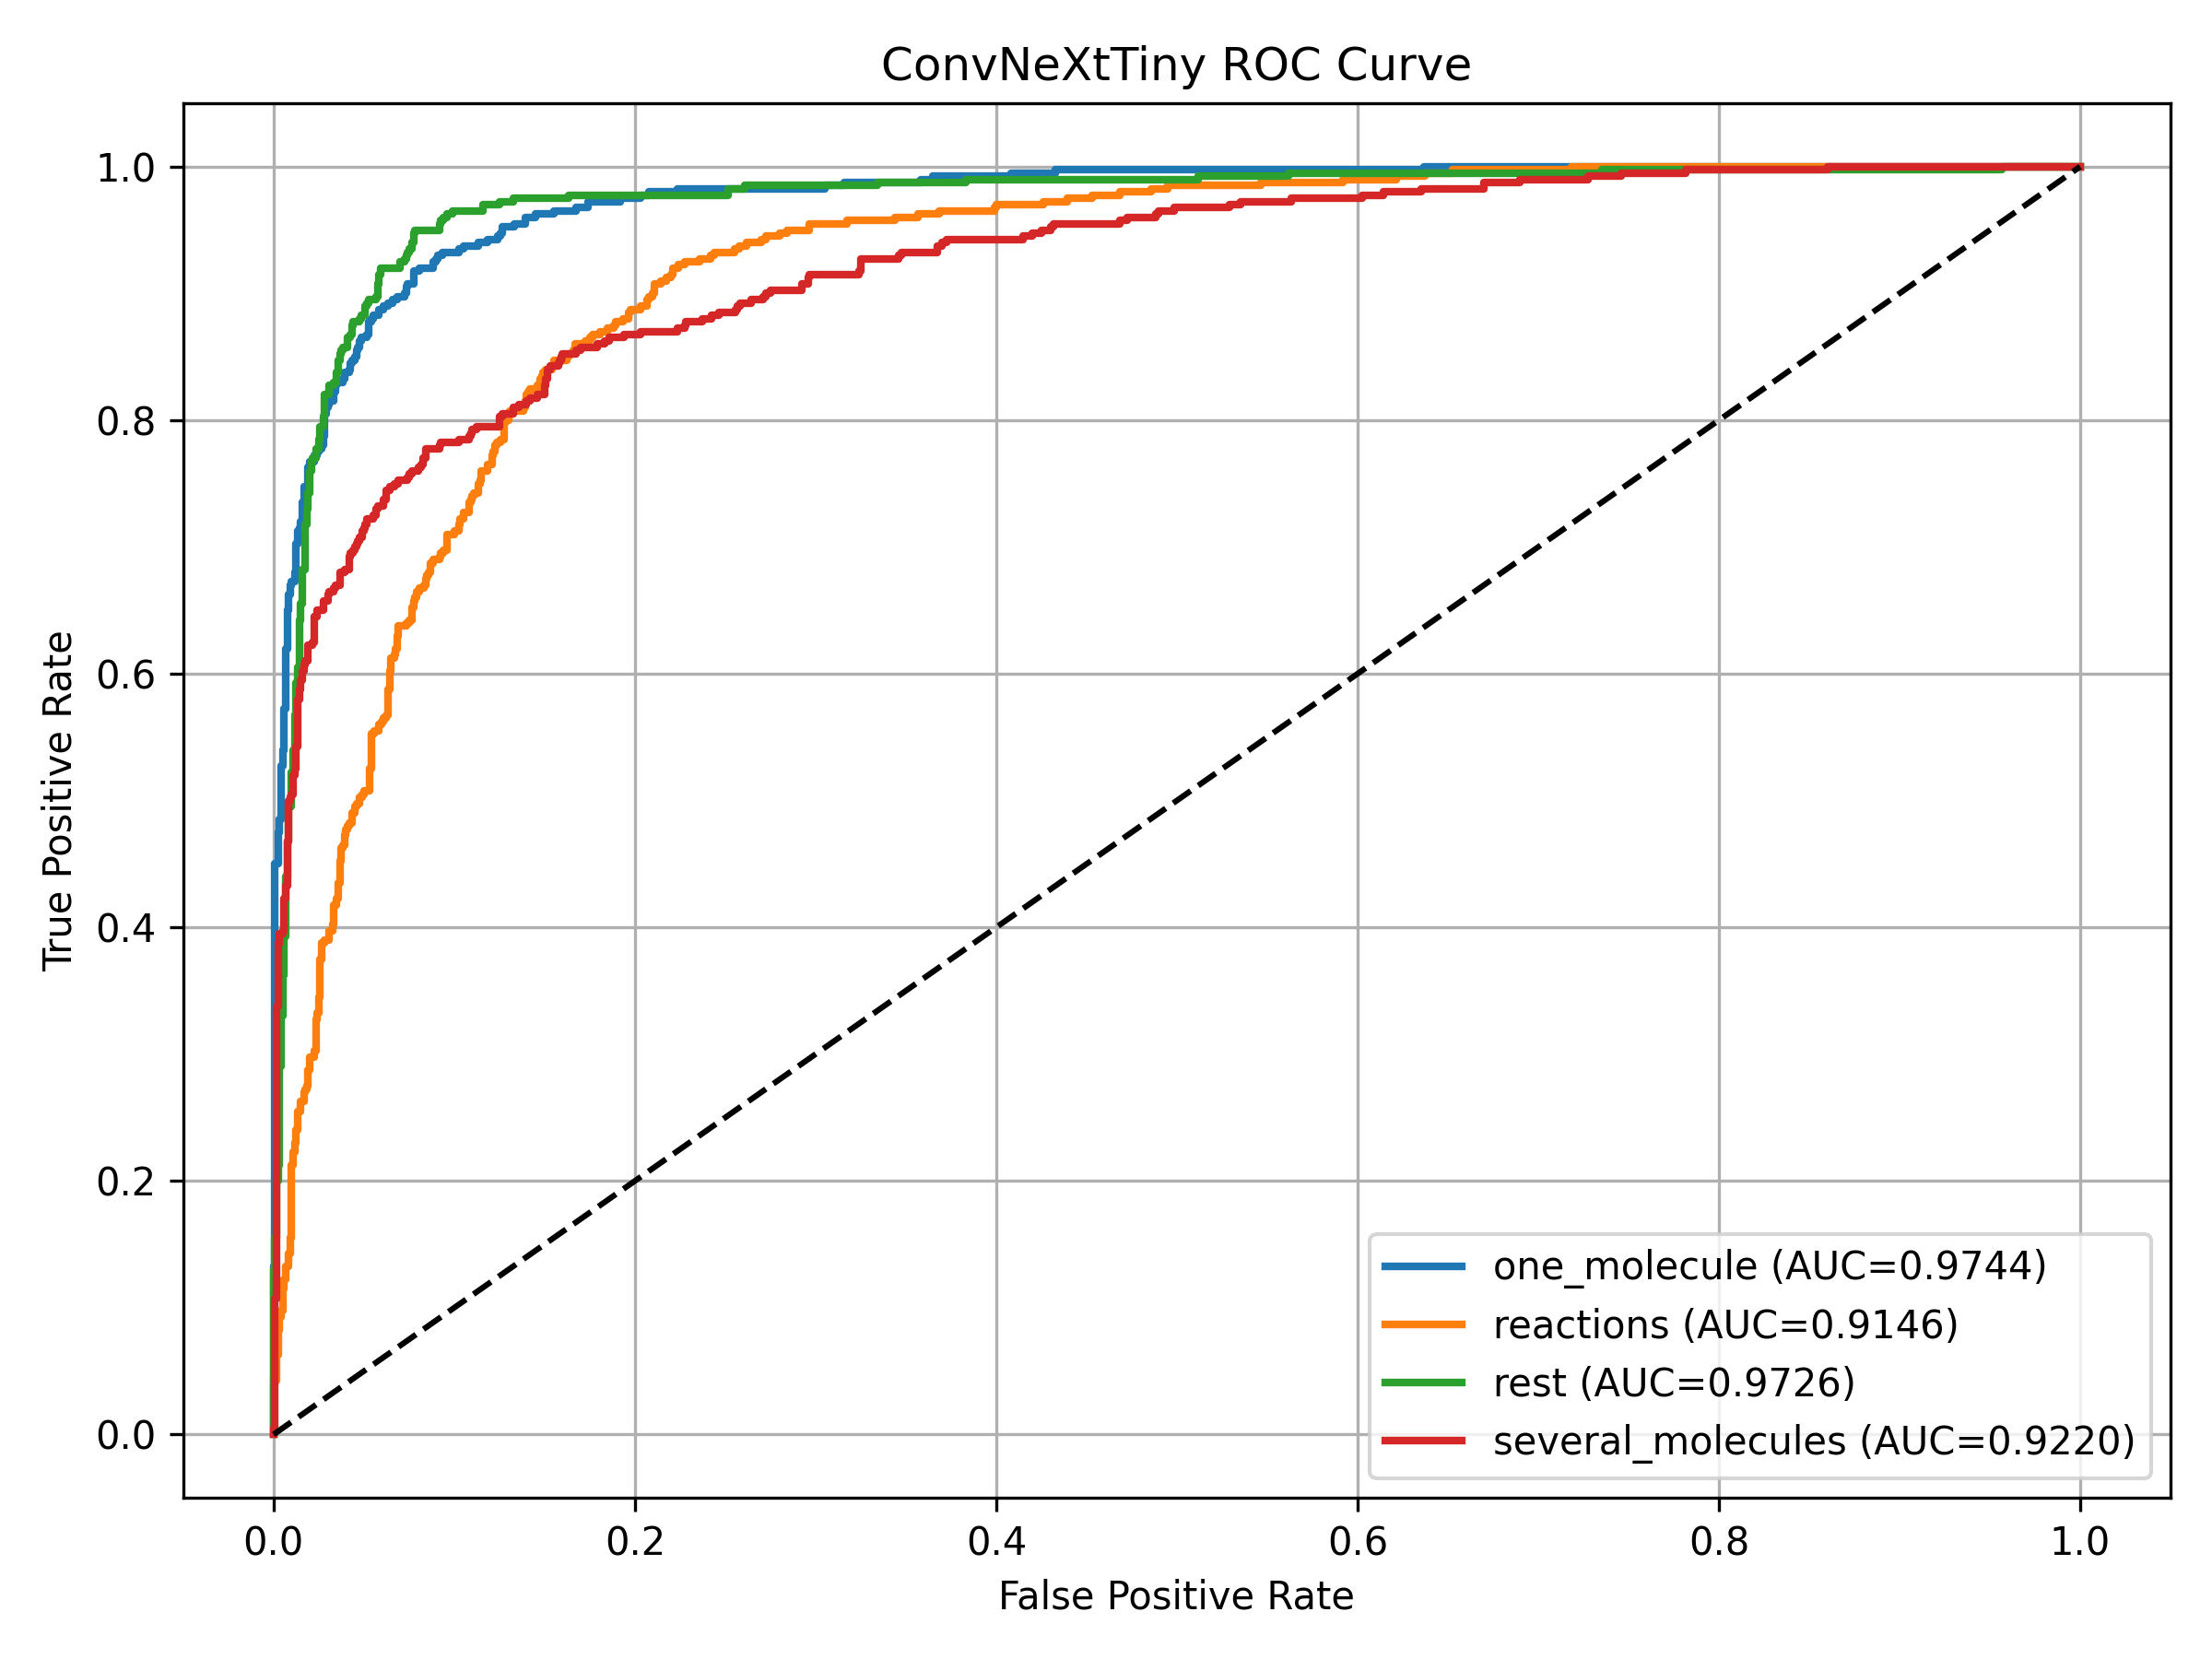
\includegraphics[width=\textwidth]{chemical_classification_models/Results/ROC_Curves/ConvNeXtTiny_ROC.png}
  \caption{ConvNeXtTiny}
  \label{fig:roc_convnext}
\end{subfigure}
\caption{One-vs-Rest (OvR) ROC Curves --- MobileNetV2, Xception, EfficientNetB4, ConvNeXtTiny}
\label{fig:roc_curves_g2}
\end{figure}

\begin{figure}[H]
\centering
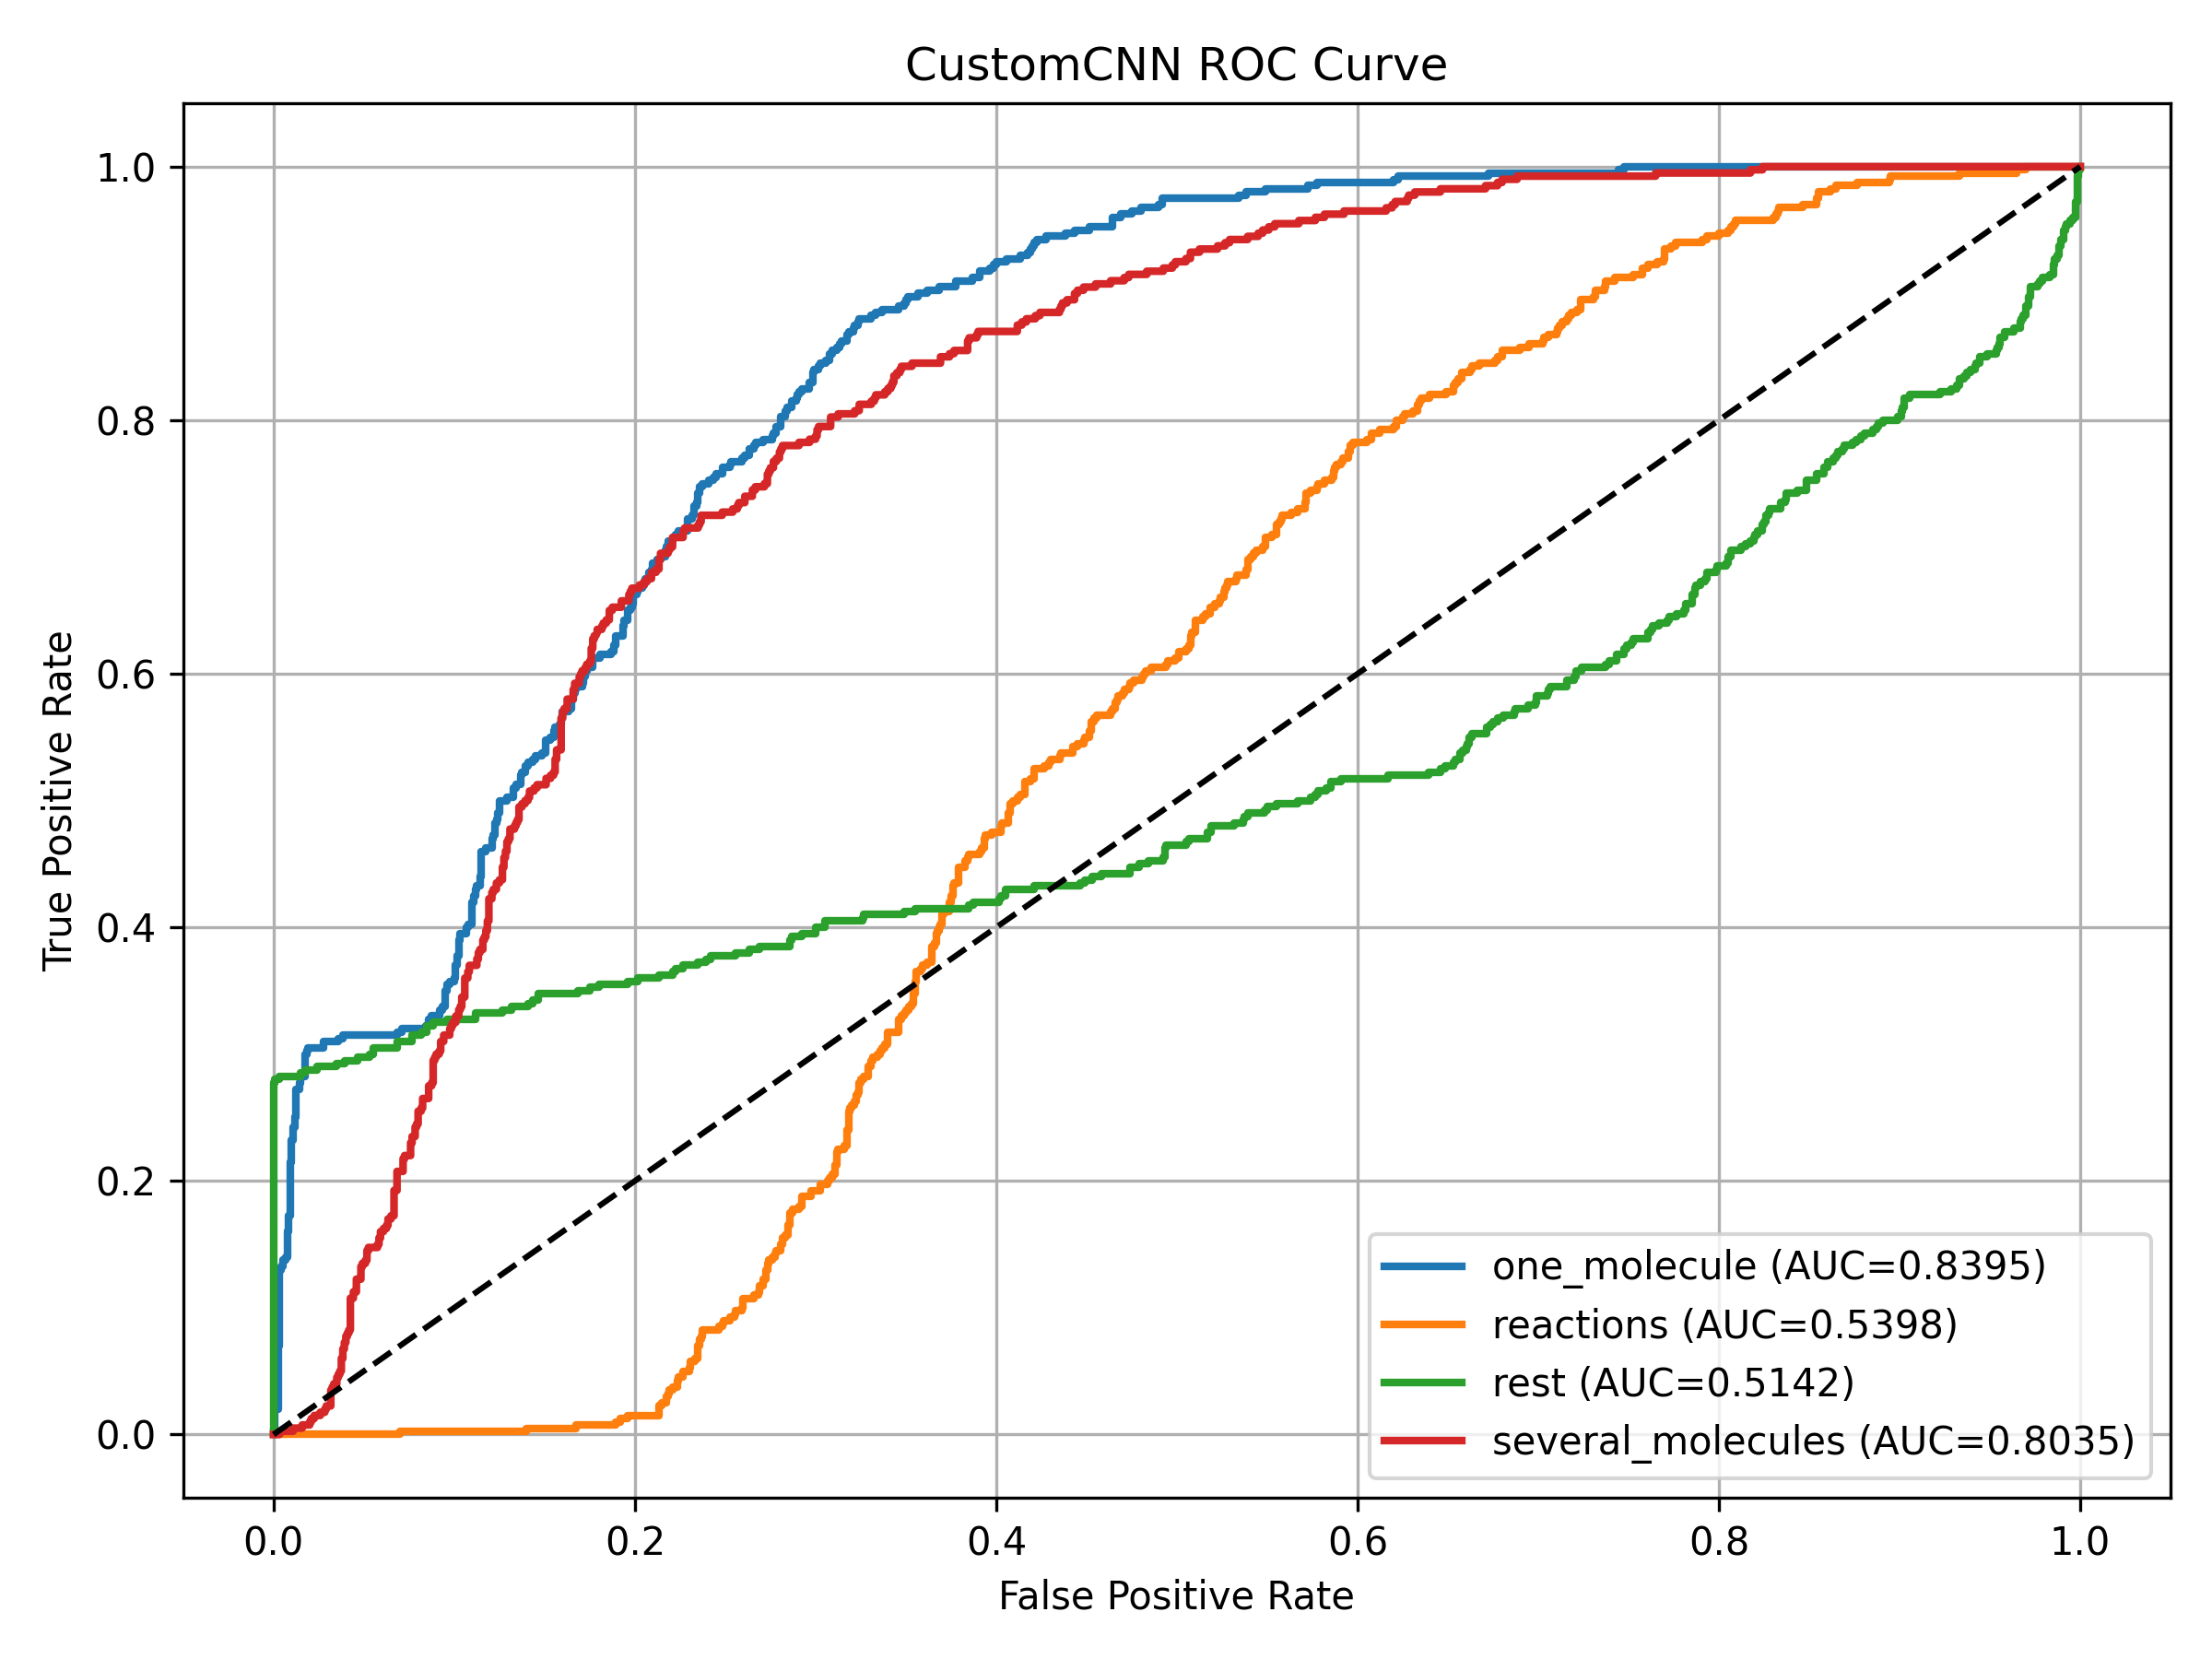
\includegraphics[width=0.66\textwidth]{chemical_classification_models/Results/ROC_Curves/CustomCNN_ROC.png}
\caption{One-vs-Rest (OvR) ROC Curve --- Custom CNN}
\label{fig:roc_custom}
\end{figure}

% ==============================================================
%  SECTION 13: GRAD-CAM
% ==============================================================
\section{Grad-CAM Visualisation}

Gradient-weighted Class Activation Mapping (Grad-CAM) was applied to VGG16 (using the \code{block5\_conv3} convolutional layer) to visualise which image regions the model focused on during classification.

\subsection{How Grad-CAM Works}

Grad-CAM computes the gradient of the predicted class score with respect to the last convolutional layer's feature maps. These gradients are global-average-pooled to produce class-discriminative weights, which are combined with the feature maps to create a heatmap. The heatmap is then overlaid on the original image using a jet colour map.

\begin{lstlisting}[language=Python, caption={Grad-CAM Implementation}]
grad_model = tf.keras.models.Model(
    inputs=[base_model.input],
    outputs=[base_model.get_layer('block5_conv3').output, base_model.output]
)
with tf.GradientTape() as tape:
    conv_outputs, predictions = grad_model(img_tensor)
    class_channel = tf.gather(predictions[0], pred_index)
grads        = tape.gradient(class_channel, conv_outputs)
pooled_grads = tf.reduce_mean(grads, axis=(0, 1, 2))
heatmap      = conv_outputs[0] @ pooled_grads[..., tf.newaxis]
heatmap      = tf.maximum(heatmap, 0) / tf.math.reduce_max(heatmap)
\end{lstlisting}

\begin{figure}[H]
  \centering
  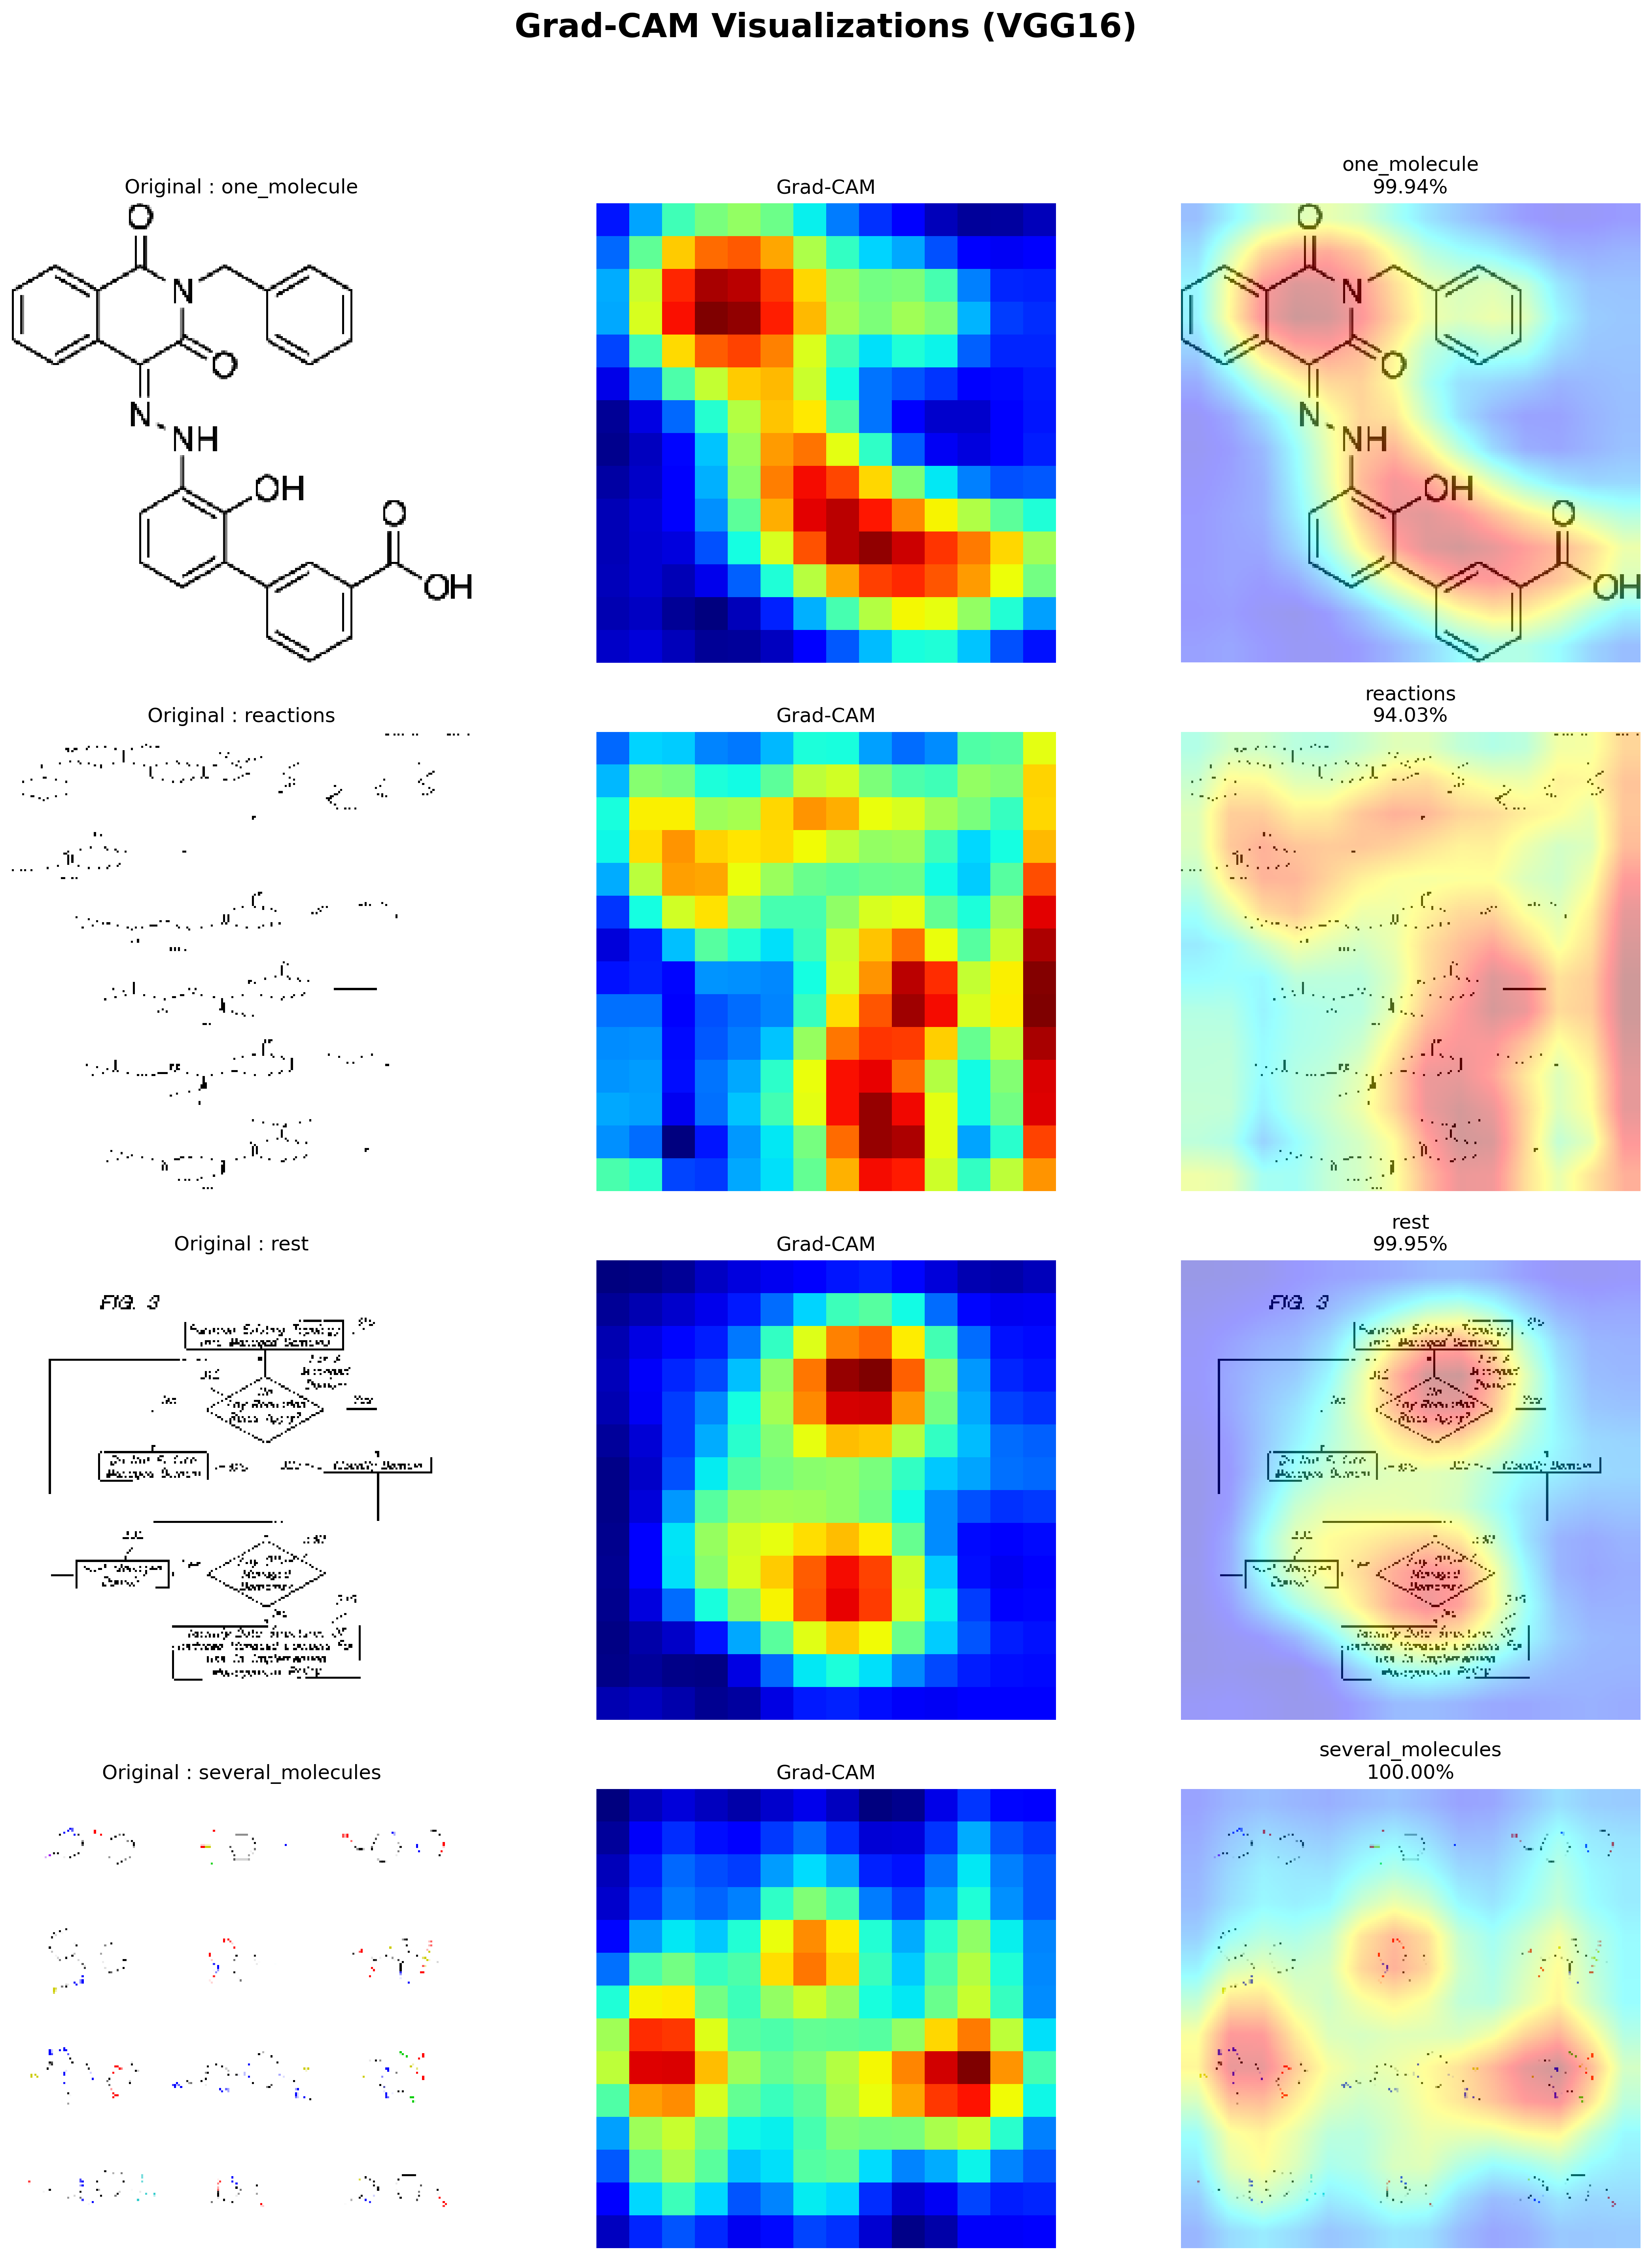
\includegraphics[width=0.88\textwidth]{chemical_classification_models/Results/Visualizations/VGG16_GradCAM.png}
  \caption{Grad-CAM Heatmaps --- VGG16 (one row per class: original image + overlay)}
  \label{fig:gradcam}
\end{figure}

\begin{notebox}[Grad-CAM Insight]
The heatmaps confirm that VGG16 correctly focuses on \textbf{molecular bonds}, \textbf{reaction arrows}, and \textbf{structural backbone patterns} --- demonstrating genuine feature learning rather than texture bias.
\end{notebox}

% ==============================================================
%  SECTION 14: LIME EXPLAINABILITY
% ==============================================================
\section{LIME Explainability}

LIME (Local Interpretable Model-agnostic Explanations) was applied to the VGG16 model. LIME perturbs the input image into superpixel segments and fits a local linear model around each prediction to identify which image regions \textit{support} or \textit{contradict} the prediction.

\subsection{Output per class (3 subplot columns)}

\begin{itemize}[leftmargin=1.6em, itemsep=4pt]
  \item \textbf{Original Image} --- raw test image from the class.
  \item \textbf{Positive Regions (Green)} --- superpixels that supported the top predicted class.
  \item \textbf{Negative Regions (Red)} --- superpixels that worked against the top prediction.
\end{itemize}

\begin{lstlisting}[language=Python, caption={LIME Image Explanation}]
explainer   = lime_image.LimeImageExplainer()
explanation = explainer.explain_instance(
    img_array.astype('double'),
    predict_fn,       # model.predict wrapper
    top_labels=4, hide_color=0, num_samples=1000
)
temp, mask = explanation.get_image_and_mask(
    top_label, positive_only=True, hide_rest=False
)
\end{lstlisting}

\begin{figure}[H]
  \centering
  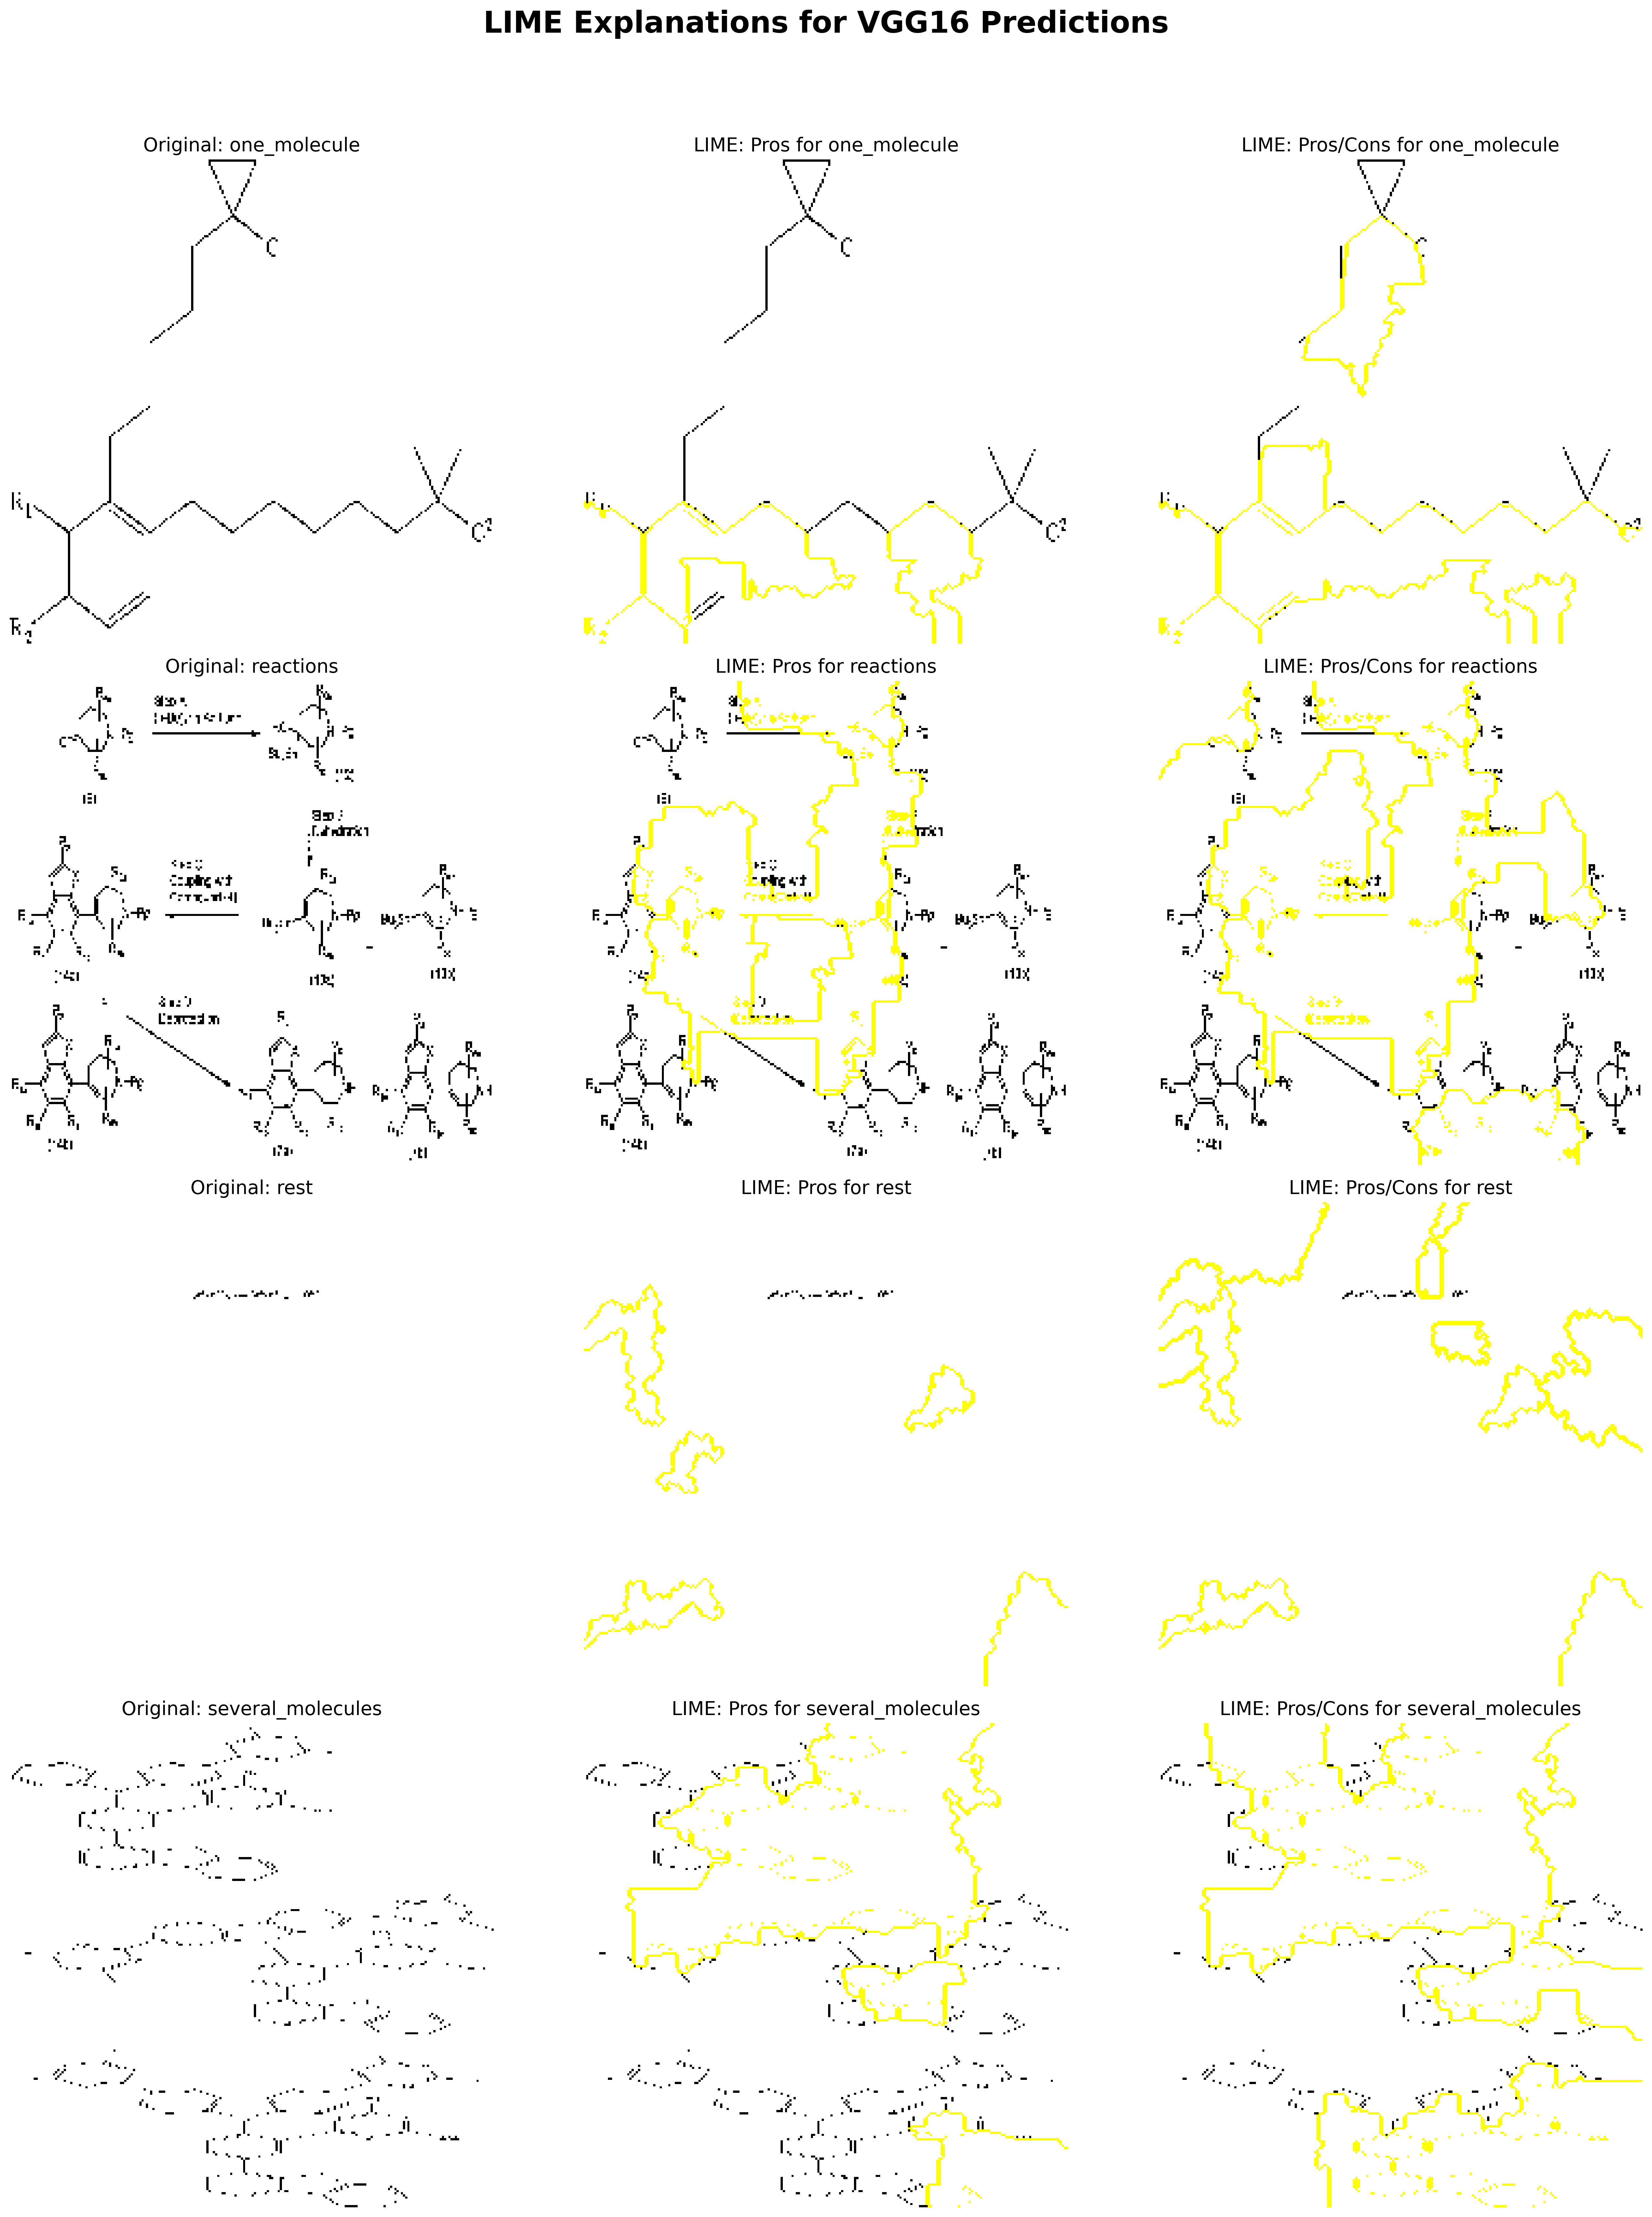
\includegraphics[width=0.88\textwidth]{chemical_classification_models/Results/Visualizations/Lime_VGG16_Fixed.png}
  \caption{LIME Explanations --- VGG16 (all 4 classes)}
  \label{fig:lime}
\end{figure}

\begin{notebox}[LIME Insight]
LIME explanations show clear \textbf{positive (green) regions} aligned with key chemical structures --- e.g., ring systems for \textit{one\_molecule} and arrows/reagent labels for \textit{reactions} --- providing interpretable evidence for each prediction.
\end{notebox}

% ==============================================================
%  SECTION 15: CONCLUSION
% ==============================================================
\section{Conclusion \& Key Findings}

This report presents a comprehensive deep learning pipeline for chemical image classification. Nine different architectures were trained and rigorously evaluated on a balanced dataset of 16,000 images. The key findings are summarised below:

\begin{itemize}[leftmargin=1.6em, itemsep=5pt]
  \item \modelname{VGG16} achieved the best overall performance (Accuracy: \textbf{91.06\%}, AUC: \textbf{0.9890}), making it the most suitable model for this task.
  \item \modelname{ResNet50V2} and \modelname{DenseNet121} also performed strongly ($\sim$89--90\% accuracy), confirming that residual and dense connection architectures transfer well to chemical imagery.
  \item \modelname{InceptionV3} (88.6\%, AUC: 0.9846) and \modelname{Xception} (80.9\%) showed competitive results using $299\times299$ input resolution.
  \item \modelname{MobileNetV2} and \modelname{ConvNeXtTiny} both achieved 76.9\% accuracy; MobileNetV2 is well-suited to deployment where model size is constrained.
  \item \modelname{EfficientNetB4} underperformed significantly (39.4\%) --- due to its built-in normalisation conflicting with the \code{rescale=1./255} generator pipeline.
  \item The \modelname{Custom CNN} achieved only 26.9\% accuracy, demonstrating that training deep networks from scratch on 12,800 images is insufficient without pre-trained features.
  \item \textbf{Grad-CAM} confirmed VGG16 correctly focused on molecular bonds, reaction arrows, and structural patterns --- validating genuine feature learning.
  \item \textbf{LIME explanations} showed clear positive (green) regions aligned with key chemical structures, providing interpretable evidence for each prediction.
\end{itemize}

\subsection{Final Model Ranking by Accuracy}

\begin{table}[H]
\centering
\caption{Final Model Ranking by Accuracy and AUC}
\label{tab:final_ranking_summary}
\rowcolors{2}{LightGray}{white}
\begin{tabular}{l l c c}
  \toprule
  \textbf{Rank} & \textbf{Model} & \textbf{Accuracy} & \textbf{AUC} \\
  \midrule
  \rowcolor{green!12} \textbf{1st} & \textbf{VGG16}    & \textbf{91.06\%} & \textbf{0.9890} \\
  2nd & ResNet50V2     & 89.88\% & 0.9821 \\
  3rd & DenseNet121    & 89.13\% & 0.9832 \\
  4th & InceptionV3    & 88.63\% & 0.9846 \\
  5th & Xception       & 80.88\% & 0.9554 \\
  6th & MobileNetV2    & 76.88\% & 0.9614 \\
  6th & ConvNeXtTiny   & 76.88\% & 0.9459 \\
  8th & EfficientNetB4 & 39.38\% & 0.7105 \\
  9th & Custom CNN     & 26.94\% & 0.6743 \\
  \bottomrule
\end{tabular}
\end{table}

\begin{insightbox}[Overall Conclusion]
Transfer learning is highly effective for chemical image classification. \textbf{VGG16}, despite being the oldest architecture tested, delivered the best results --- likely because its large receptive fields and sequential deep feature hierarchy are well-suited to capturing structural chemistry patterns. Future work should explore ensemble methods, larger datasets, or domain-specific pre-training to push accuracy beyond 95\%.
\end{insightbox}

\vspace{2em}
\begin{center}
  \color{DarkGray}\sffamily\small --- End of Report ---
\end{center}

\end{document}
